\documentclass[8pt]{beamer}
\usepackage[T1]{fontenc} 
\usepackage[francais]{babel}
\usepackage{tikz}
\usetikzlibrary{arrows,shapes}
\usepackage{pslatex}
\usepackage{textcomp}
\usepackage[utf8]{inputenc}
\usepackage{wrapfig}
\usepackage{graphicx}
\usepackage[section]{placeins}
\usepackage{lscape}
\usepackage{float} 
\usepackage{amssymb}
\usepackage{wasysym}
\usepackage{pgf}
\usepackage{alltt}
\usepackage{eso-pic}
\usepackage{comment}
\usepackage{ulem}
\usepackage{multirow}
\usepackage{xcolor,colortbl}
\usepackage{pstricks}

\definecolor{MyGray}{gray}{0.85}

\usetheme{Frankfurt}

\graphicspath{{figs/}}

\title[Séminaire 2ieme année]{Développement d'un algorithme de suivi \\ de particules (PFA) pour l'ILC. Outils de monitoring \\ en ligne de qualité de données}
\subtitle{Séminaire de 2ième année}
\institute[UCBL - IPNL]{Université Claude Bernard Lyon 1 \\ Institut de Physique Nucléaire de Lyon }
\author[R. Eté]{{\bf Eté Rémi}}
\date{9 octobre 2015}

\DeclareUnicodeCharacter{00A0}{ }

\setbeamertemplate{itemize items}[ball]
%\addtobeamertemplate{block begin}{\pgfsetfillopacity{0.5}}{\pgfsetfillopacity{1}}

\begin{document}

  %%%%%%%%%%%%%% Page de présentation %%%%%%%%%%%%%%
  \begin{frame}

    \titlepage
    \begin{center} 
      
\includegraphics[width=0.2\textwidth]{logo_ipnl.jpg} ~~~
      
\includegraphics[width=0.2\textwidth]{logo_calice.png} ~~~
      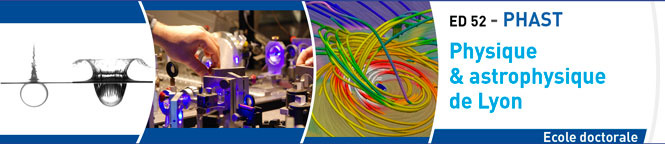
\includegraphics[width=0.5\textwidth]{logo-edphast.jpg}
    \end{center}
  \end{frame}


  \begin{frame}
  \frametitle{Sommaire}
    \tableofcontents
  \end{frame}   

%%%%%%%%%%%%%%%%%%
%% INTRODUCTION %%
%%%%%%%%%%%%%%%%%%

  \section{Introduction}
  
  \begin{frame}
  \frametitle{\secname}
    \tableofcontents[currentsection]
  \end{frame}

  \subsection{Le modèle standard}
  
  %% Modele standard
  \begin{frame}
  \frametitle{\secname}
  \framesubtitle{Le modèle standard}
    \begin{minipage}{0.6\linewidth}
      \begin{block}{Le modèle standard}
        Théorie unifiant 3 des 4 interactions fondamentales :
        \begin{itemize}
          \item L'interaction électromagnétique
          \item L'interaction faible
          \item L'interaction forte
        \end{itemize}
        Théorie de jauge SU(3) $\bigotimes$ SU(2) $\bigotimes$ U(1)
      \end{block}
    \end{minipage} \hfill
    \begin{minipage}{0.38\linewidth}
      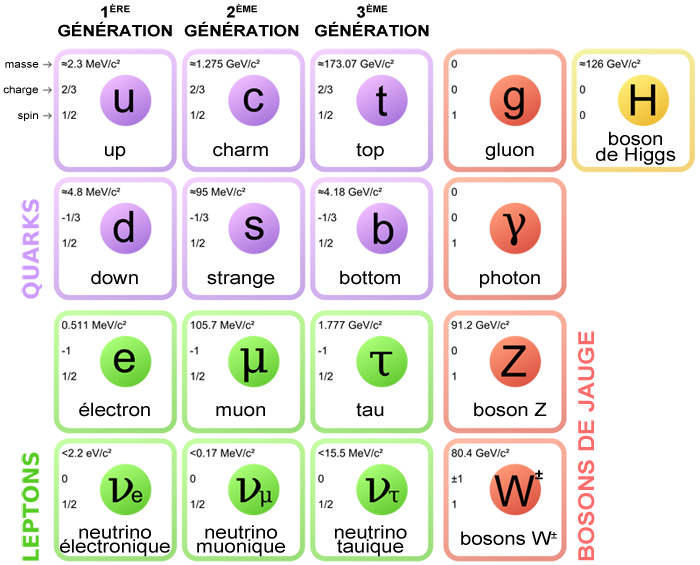
\includegraphics[width=0.9\linewidth]{Particules_elementaires.png}
    \end{minipage}
    \begin{minipage}{0.48\linewidth}
      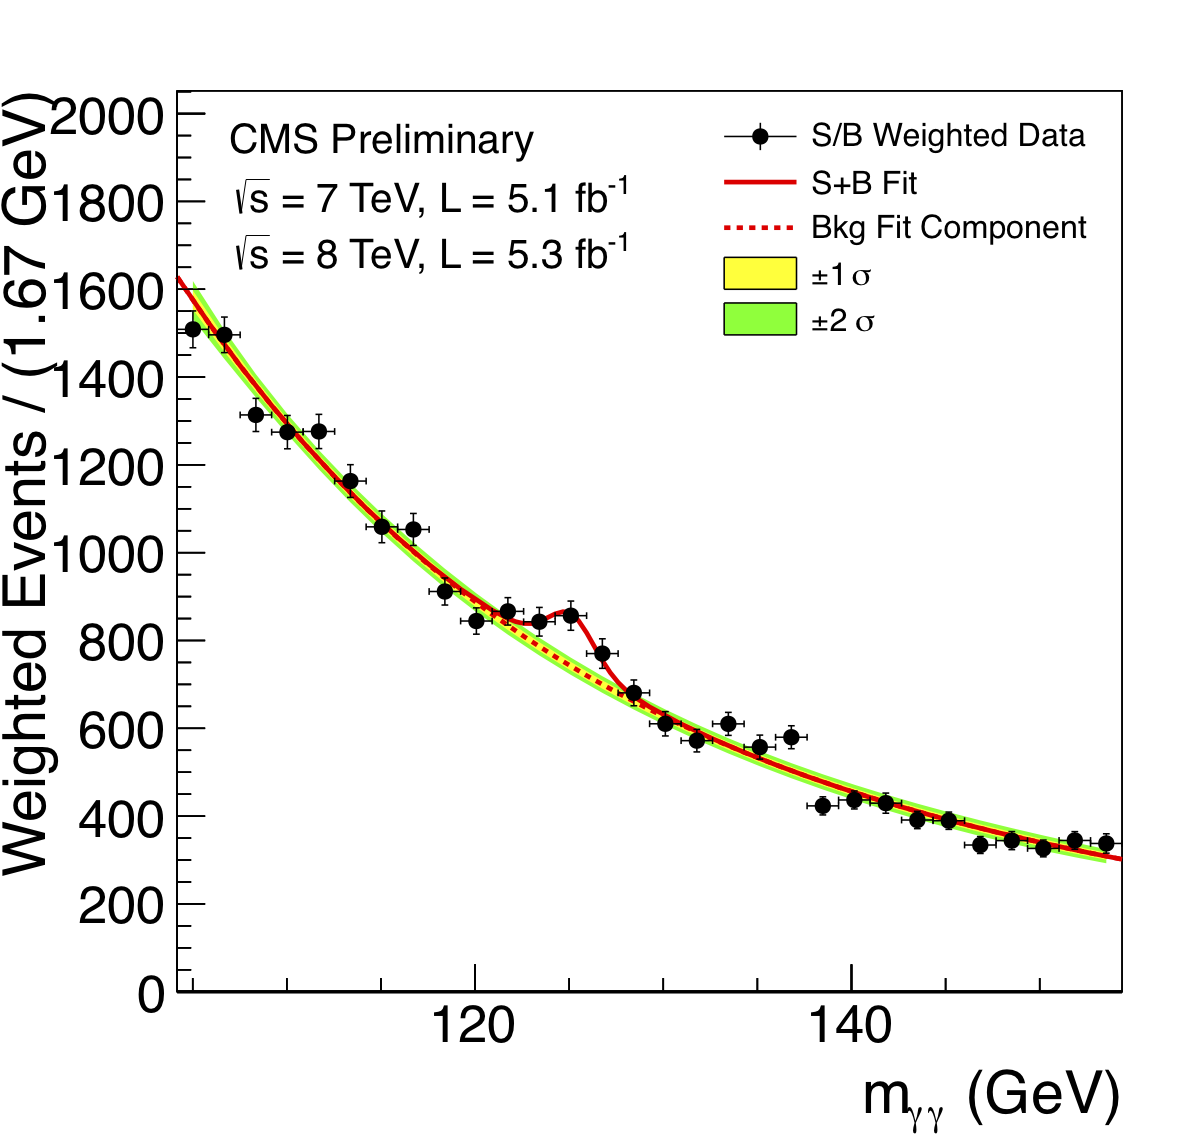
\includegraphics[width=0.9\linewidth]{CMS_Higgs_plot.png}
    \end{minipage}    
    \begin{minipage}{0.48\linewidth}
      \begin{block}{Des familles et des générations !}
        \begin{itemize}
          \item 12 fermions
          \item 4 bosons de jauge
          \item 1 boson de Higgs
        \end{itemize}
      \end{block}
      \begin{block}{Modèle incomplet}
        \begin{itemize}
          \item Pas de gravitation
          \item Masse/oscillation neutrinos
          \item Asymétrie matière/anti-matière
        \end{itemize}
      \end{block}
    \end{minipage}
  \end{frame}
  
  
  \subsection{Le collisionneur linéaire international}
  
  %% L'ILC
  \begin{frame}
  \frametitle{\secname}
  \framesubtitle{Le collisionneur linéaire international - ILC}
    \begin{center}
      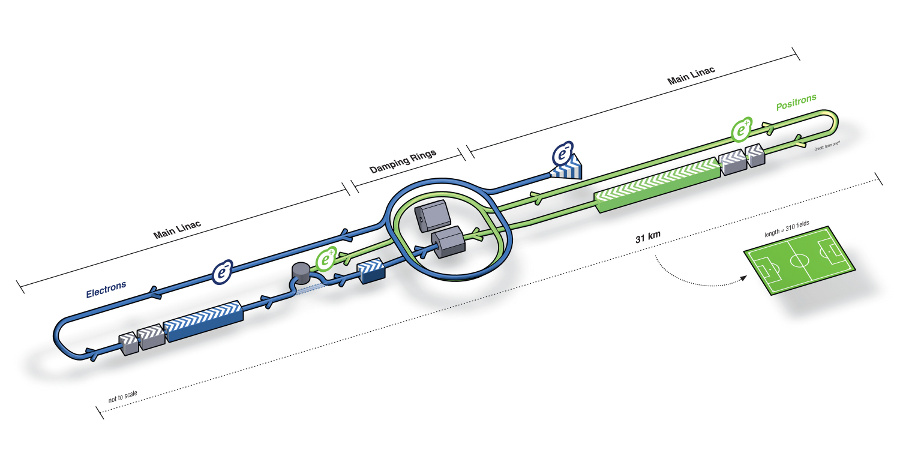
\includegraphics[width=0.6\linewidth]{ilc_layout.jpg}
    \end{center}
    \begin{minipage}{0.51\linewidth}
      \begin{block}{Caractéristiques du collisionneur}
        \begin{itemize}
          \item Collision e$^{+}$ e$^{-}$
          \item Energie : 250-500 GeV (1 TeV ?)
          \item Luminosité : 0.75$\cdot$10$^{34}$-1.8$\cdot$10$^{34}$ cm$^{-2}$s$^{-1}$
          \item Fréquence de collisions : 5 Hz (contre 40 MHz au LHC)
          \item Nb de particules par croisement : 2 $\cdot$ 10$^{10}$
          \item Alimentation pulsée
        \end{itemize}
      \end{block}
    \end{minipage} \hfill
    \begin{minipage}{0.46\linewidth}
      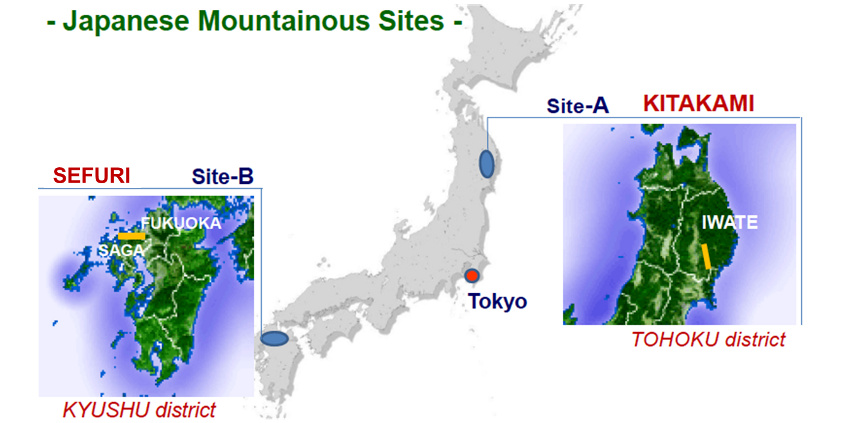
\includegraphics[width=\linewidth]{japanese_sites.jpg}
    \end{minipage}
  \end{frame}
  
  %% Le programme de l'ILC
  \begin{frame}
  \frametitle{\secname}
  \framesubtitle{Le programme physique}
    \begin{center}
      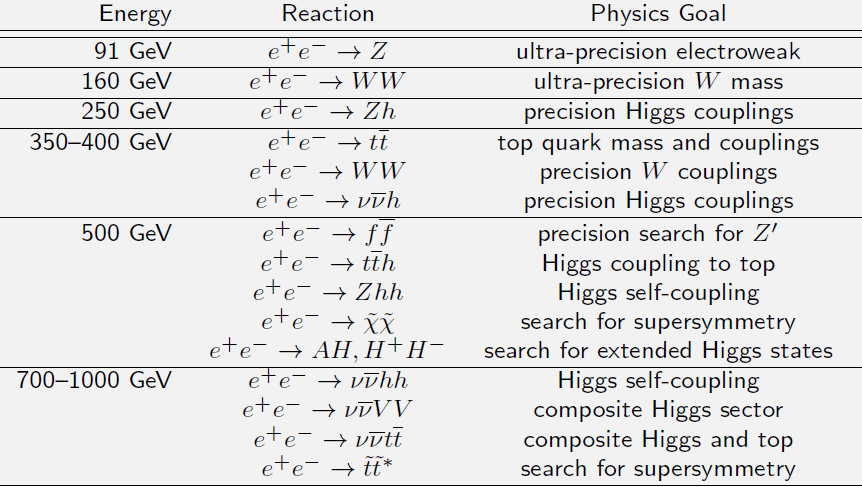
\includegraphics[width=\linewidth]{ilc_program.png}
    \end{center}
  \end{frame}
  
  %% ILD et SiD
  \begin{frame}
  \frametitle{\secname}
  \framesubtitle{ILD et SiD}
    \begin{minipage}{0.54\linewidth}
      Deux détecteurs génériques :
      \begin{itemize}
        \item ILD : TPC, plus large, B = 3.5 - 4 T
        \item SiD : Tracker en silicium, plus compact, B = 5 T
      \end{itemize}
      ~ \\
      Installation sur rail coulissant
    \end{minipage}
    \begin{minipage}{0.45\linewidth}
      \begin{center}
        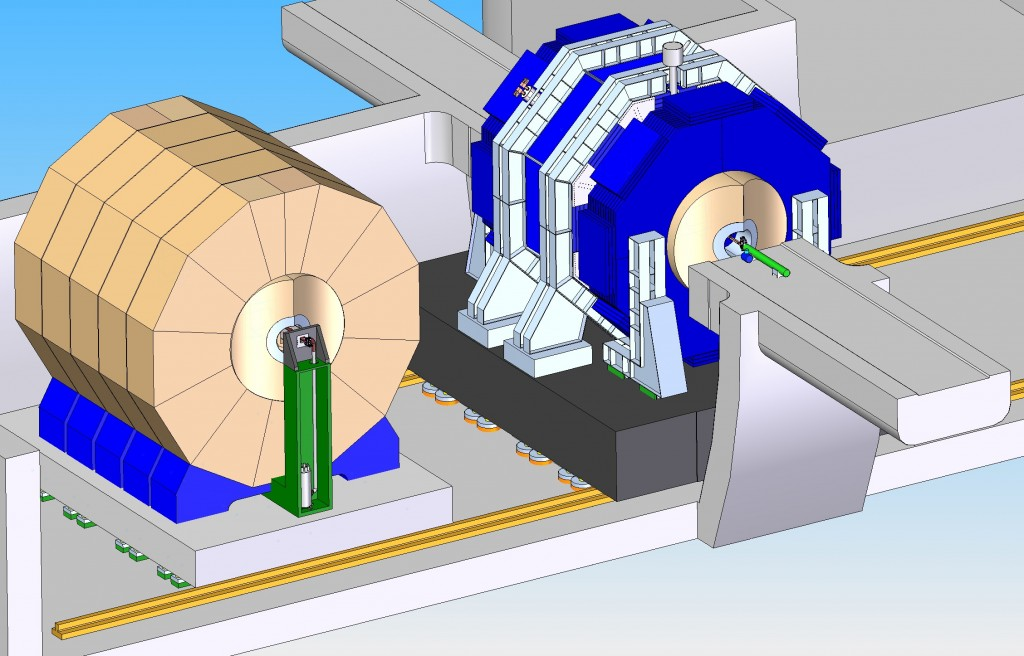
\includegraphics[width=0.94\linewidth]{ild_sid.jpg}
      \end{center}
    \end{minipage}
    ~ \\
    ~ \\
    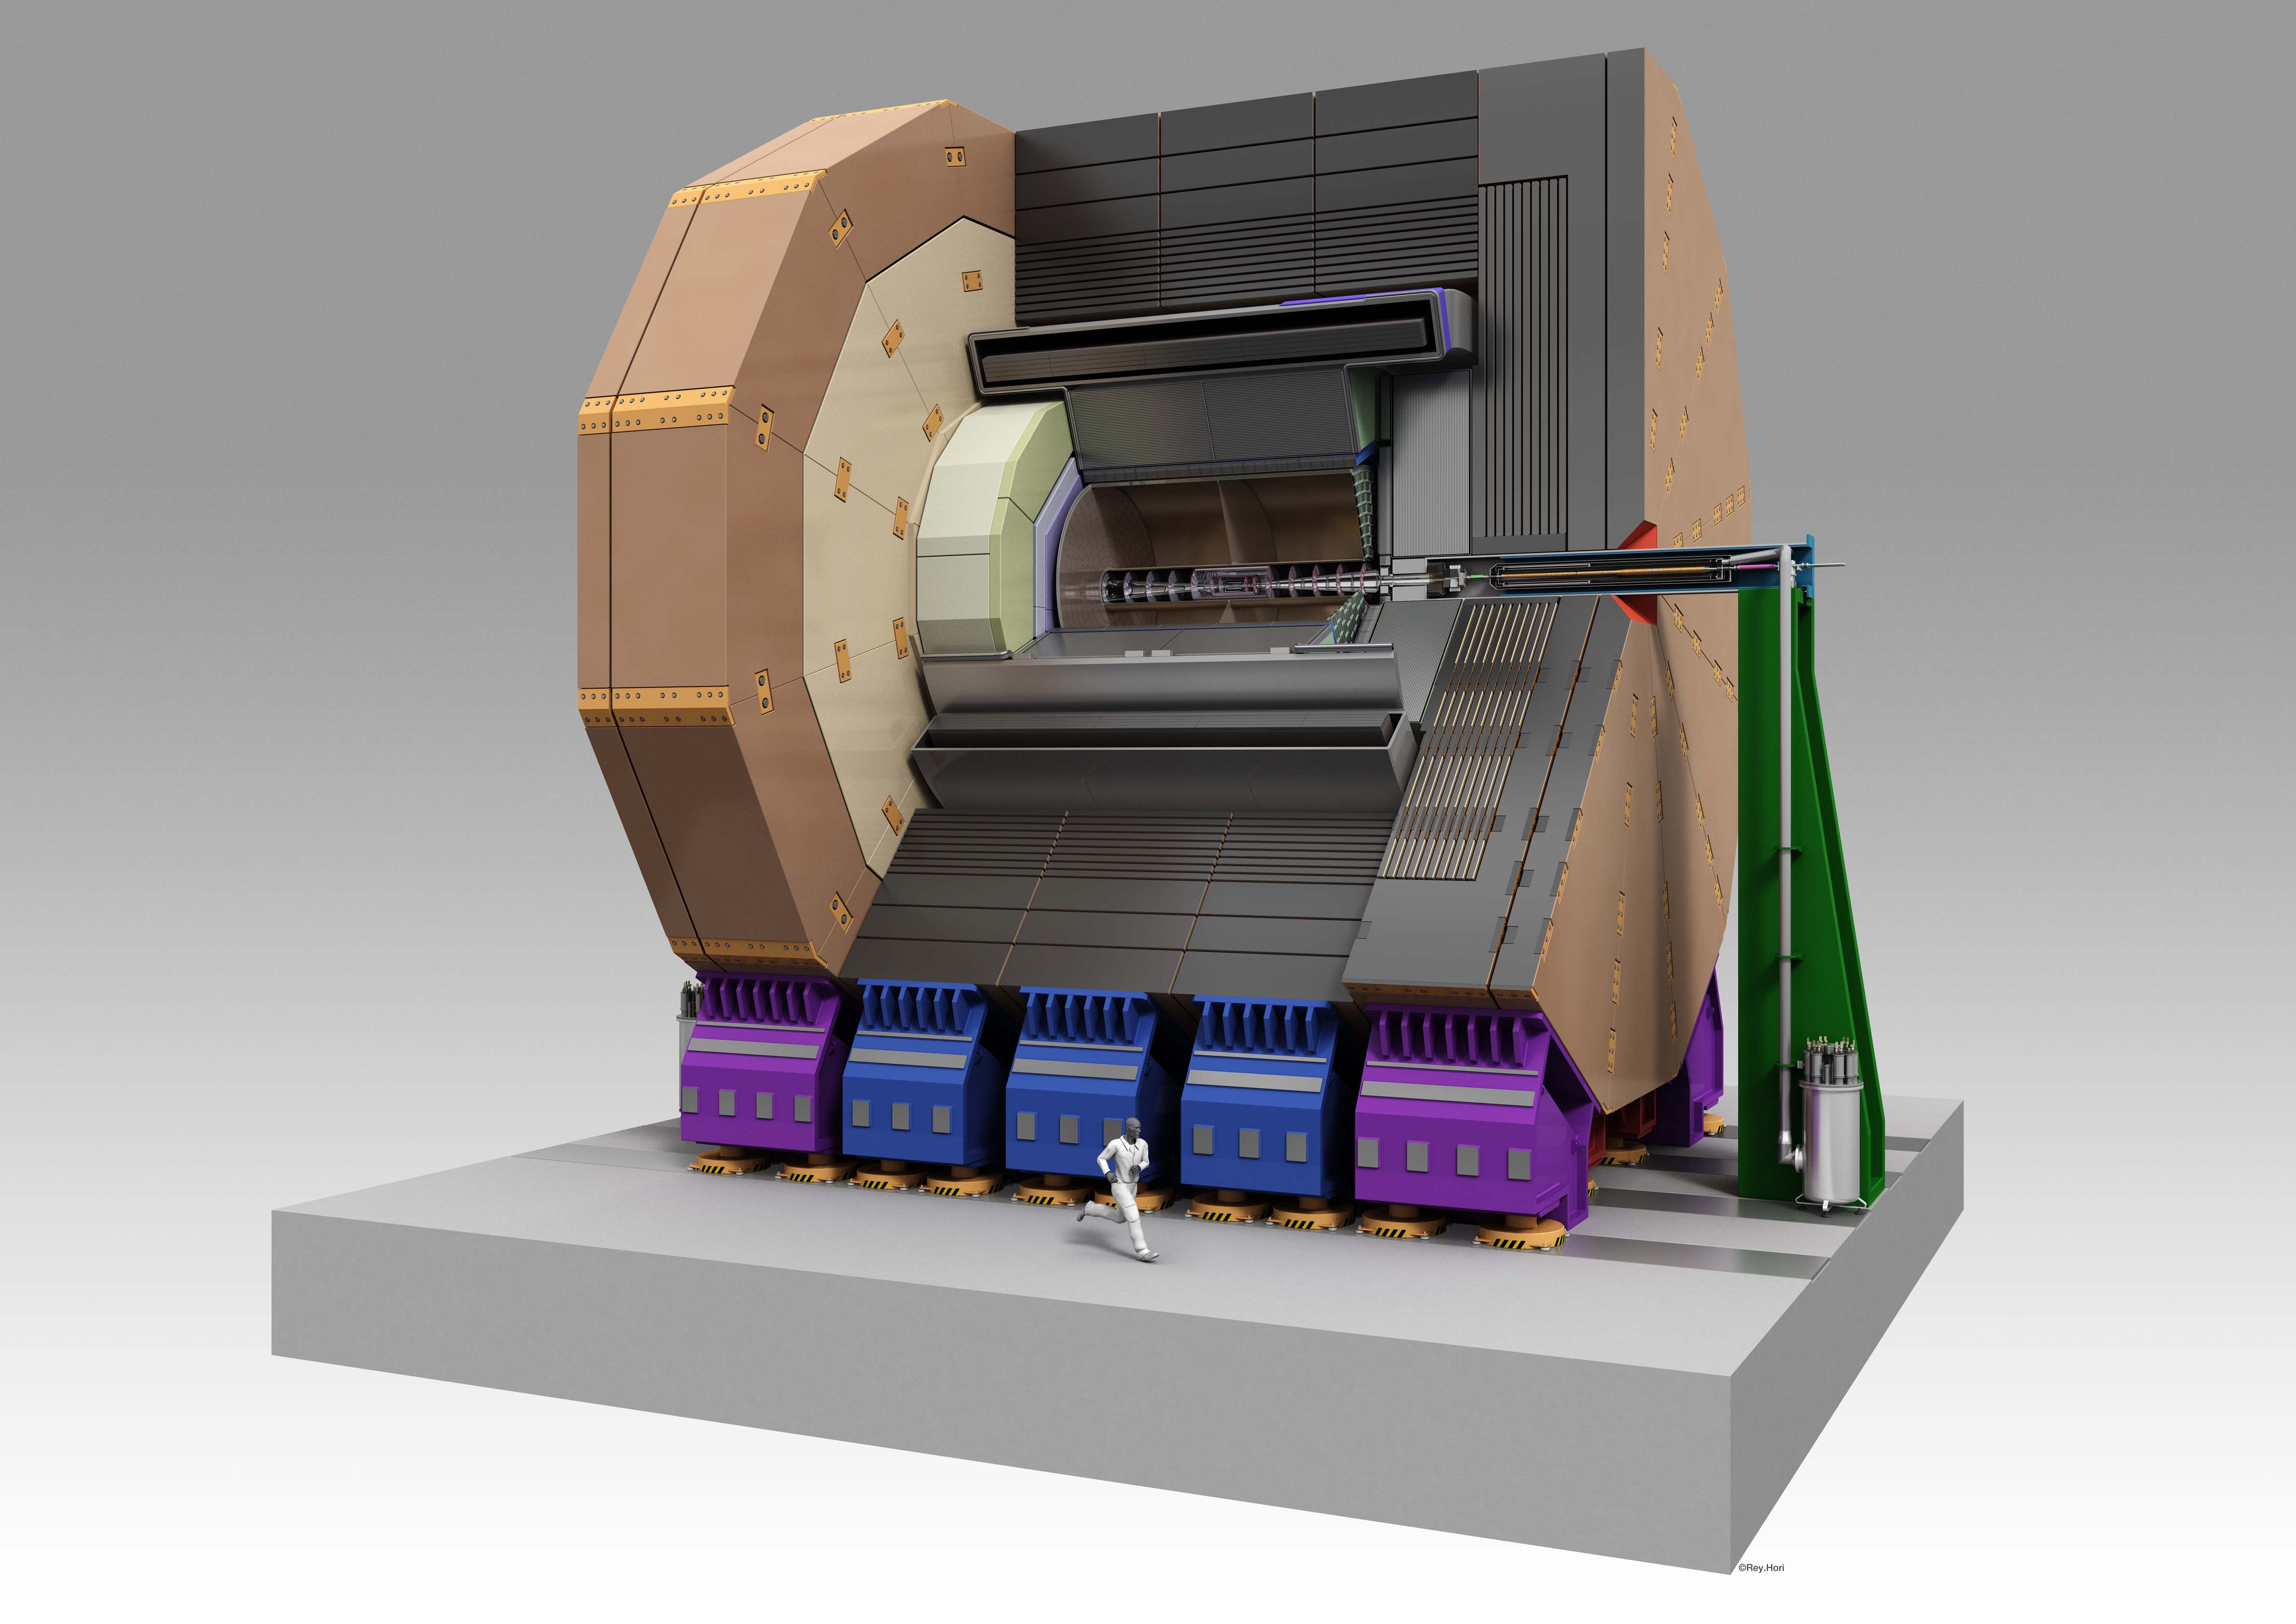
\includegraphics[width=0.48\linewidth]{ild.jpg} ~~~~
    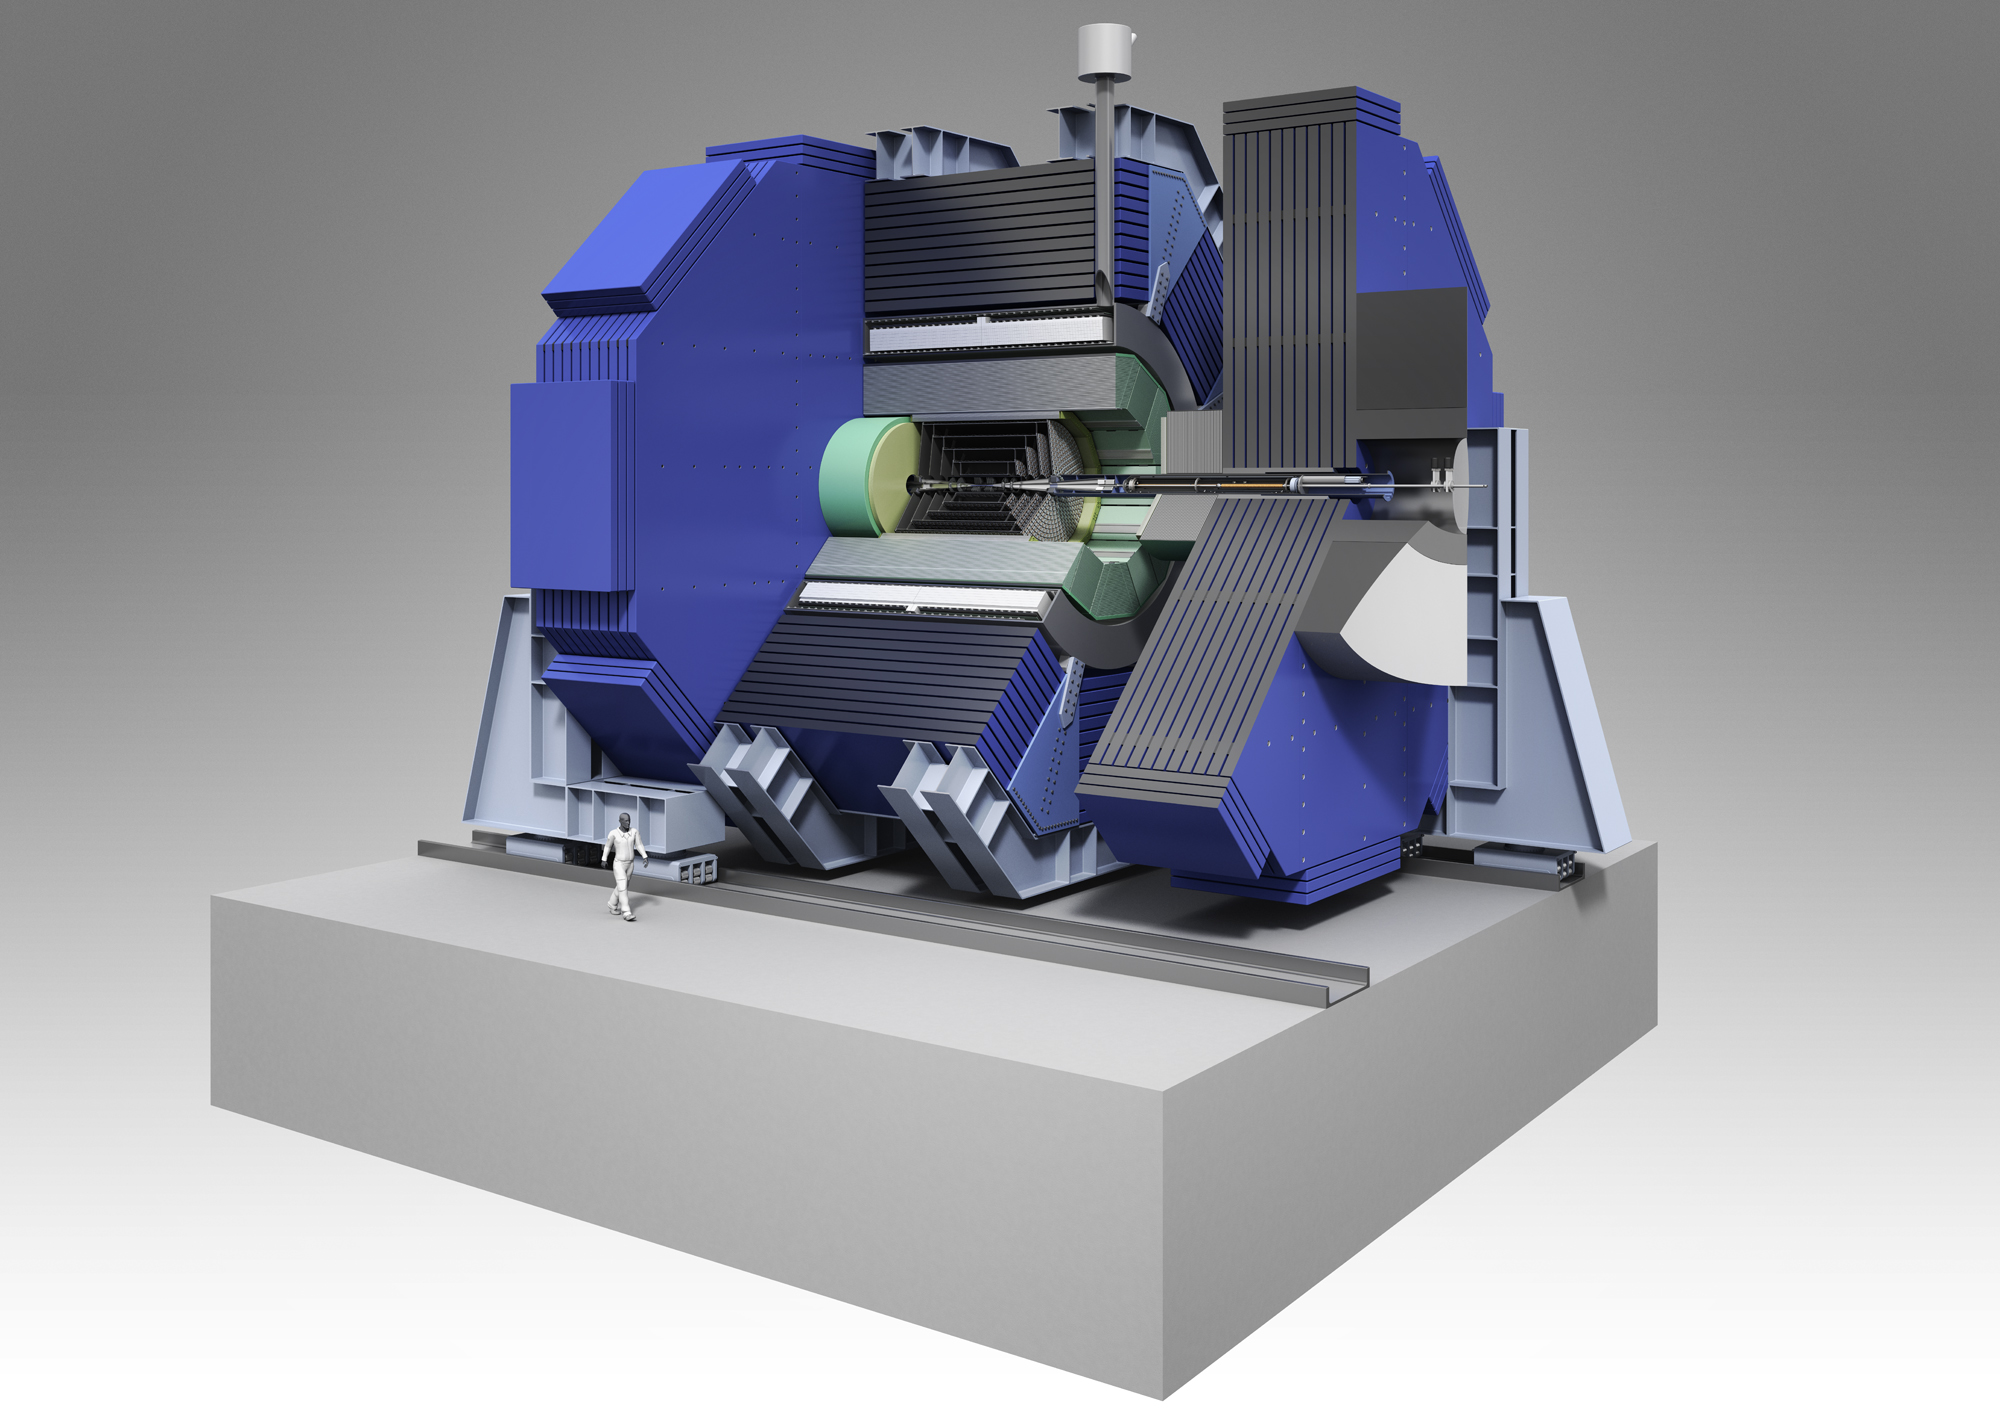
\includegraphics[width=0.48\linewidth]{sid.jpg}
  \end{frame}

  
  %% Les sous détecteurs
  \begin{frame}
  \frametitle{\secname}
  \framesubtitle{Les sous détecteurs de l'ILD}
    \begin{minipage}{0.62\linewidth}
      \begin{table}
        \begin{tabular}{c|c|c}
          \hline
          \multicolumn{1}{c}{Détecteur} & \multicolumn{1}{c}{Mesure} & \multicolumn{1}{c}{Performance} \\ 
          \hline \hline
          Trajectographe & 1 / $\delta_p$                           & 10$^{-5}$ (GeV/c)$^{-1}$ \\
          Tracking + Calo (jet)   & $\frac{\Delta E}{E}$                     & 3-4 \% \\ 
          \multirow{3}{*}{Vertex}         & {\footnotesize Résolution spatial}       & {\footnotesize < 3 $\mu m$} \\ 
          ~              & {\footnotesize Budget matière}           & {\footnotesize < 0.15 \% $X_{0}$/layer} \\
          ~              & {\footnotesize Rayon premier layer}      & {\footnotesize $\simeq$ 1.6 $cm$}
        \end{tabular}
      \end{table}
    \end{minipage} \hfill
    \begin{minipage}{0.36\linewidth}
      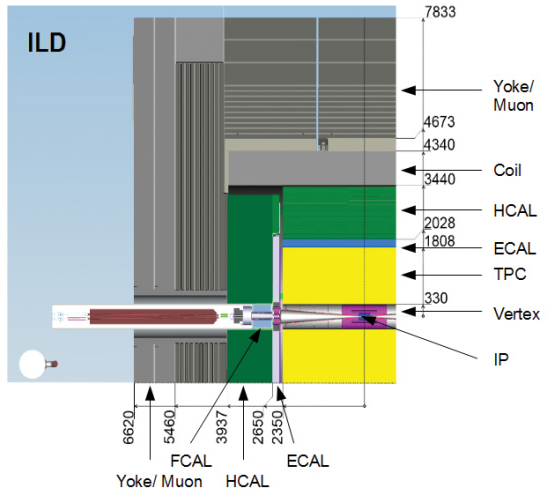
\includegraphics[width=\linewidth]{ild_vue_en_coupe.png}
    \end{minipage}
    \begin{minipage}[h]{0.5\linewidth}
      \begin{block}{Des calorimètres pour le suivi de particules}
        \begin{itemize}
          \item ECAL (résolution $\simeq 12\%/\sqrt{E}$) :
          \begin{itemize}
            \item SiWECal : 5 x 5 $mm^2$
            \item ScWECal : 5 x 45 $mm^2$ + SSA
          \end{itemize}
          \item HCAL (résolution $\simeq 60\%/\sqrt{E}$) :
          \begin{itemize}
            \item AHCAL : 3 x 3 $cm^2$
            \item SDHCAL : 1 x 1 $cm^2$
          \end{itemize}
        \end{itemize}
      \end{block}  
    \end{minipage} \hfill
    \begin{minipage}[h]{0.48\linewidth}
      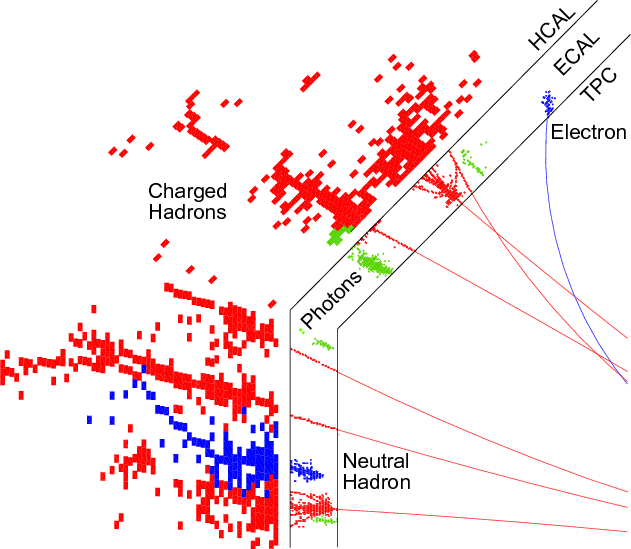
\includegraphics[width=0.8\linewidth]{pfa_event_display.png}
    \end{minipage}
  \end{frame}

  %% Le prototype SDHCAL
  \subsection{Le calorimètre hadronique semi-digital}
  
  \begin{frame}
  \frametitle{\secname}
  \framesubtitle{\subsecname}
    \begin{minipage}{0.48\linewidth}
      \begin{block}{Semi-Digital Hadron Calorimeter}
        \begin{itemize}
          \item Calorimètre à échantillonnage
          \item 48 plans :
          \begin{itemize}
            \item Absorber en acier
            \item Milieu sensitif : GRPC
          \end{itemize}
          \item Segmentation :
          \begin{itemize}
            \item Transverse : 1 $cm^2$
            \item Longitudinale : 2.67 cm (abs. + sens)
          \end{itemize}
          \item Lecture semi-digitale à 3 seuils
        \end{itemize}
      \end{block}     
    \end{minipage} \hfill
    \begin{minipage}{0.48\linewidth}
      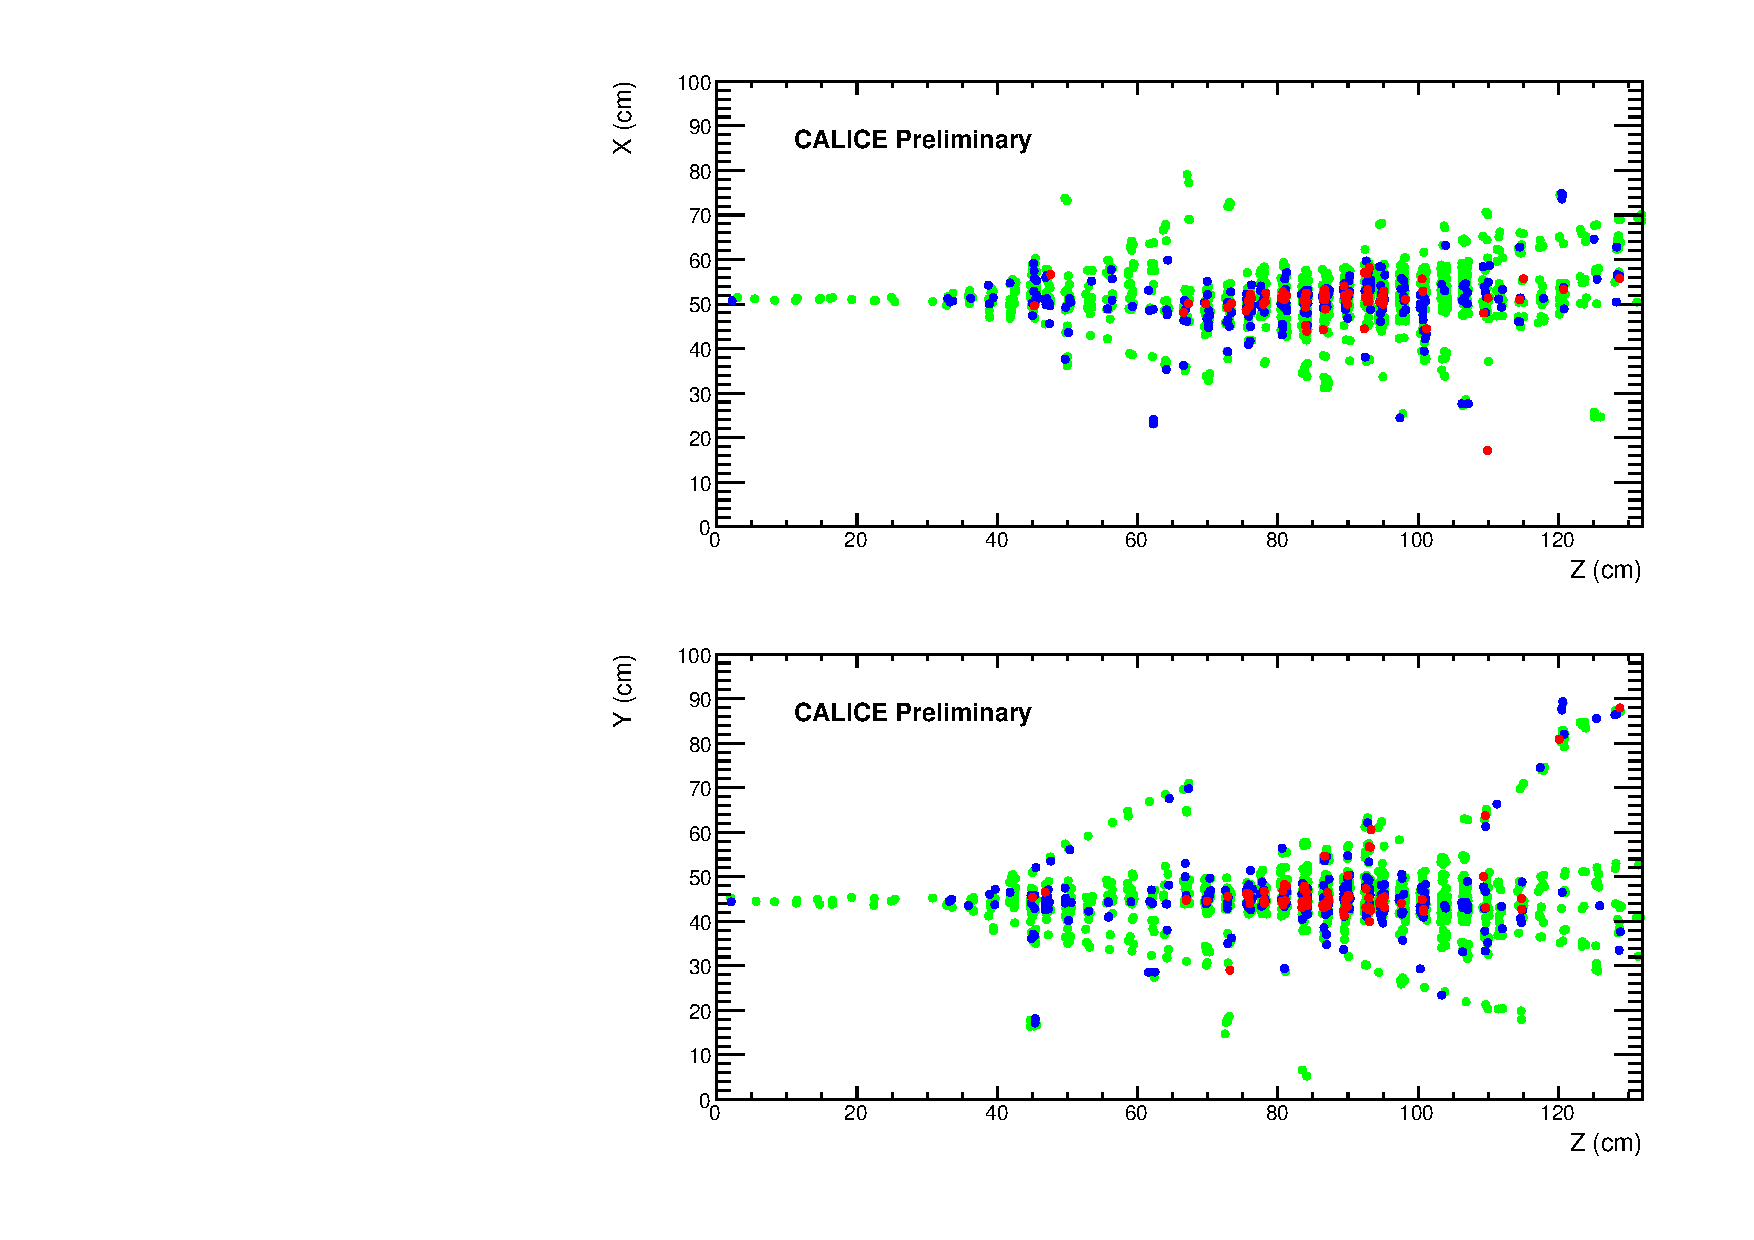
\includegraphics[width=\linewidth]{sdhcal_pion_80GeV.pdf}
    \end{minipage}
    \begin{minipage}{0.58\linewidth}
      \begin{center}
        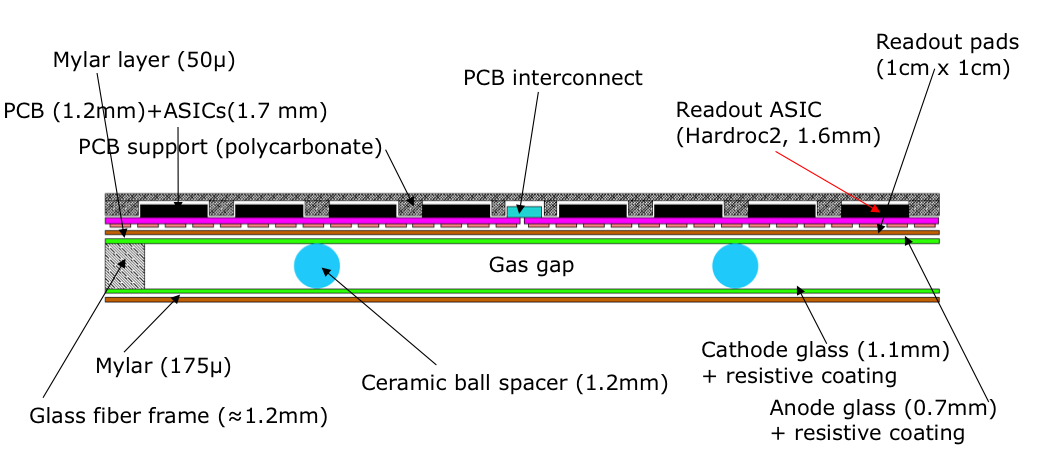
\includegraphics[width=0.9\linewidth]{GRPC-K7.png}      
      \end{center}
    \end{minipage} \hfill
    \begin{minipage}{0.4\linewidth}
      \begin{center}
        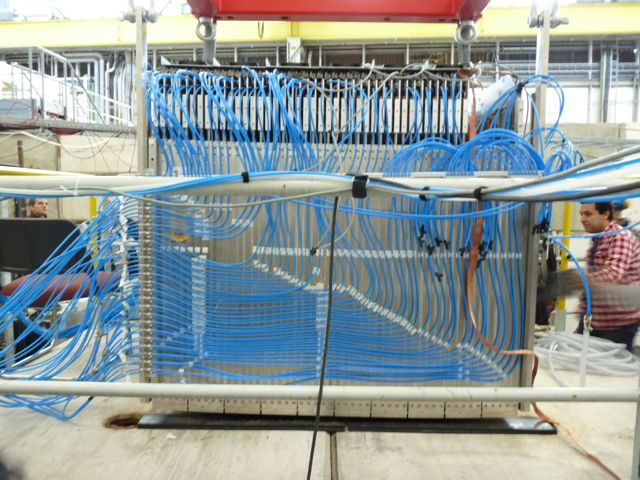
\includegraphics[width=0.7\linewidth]{sdhcal_testbeam.jpg}
      \end{center}
    \end{minipage}
  \end{frame}

  
  %% Performances du SDHCAL
  \subsection{Performances du SDHCAL}
  
  %% Multiplicité / Efficacité
  \begin{frame}
  \frametitle{\secname}
  \framesubtitle{\subsecname}
    \begin{minipage}{0.48\linewidth}
      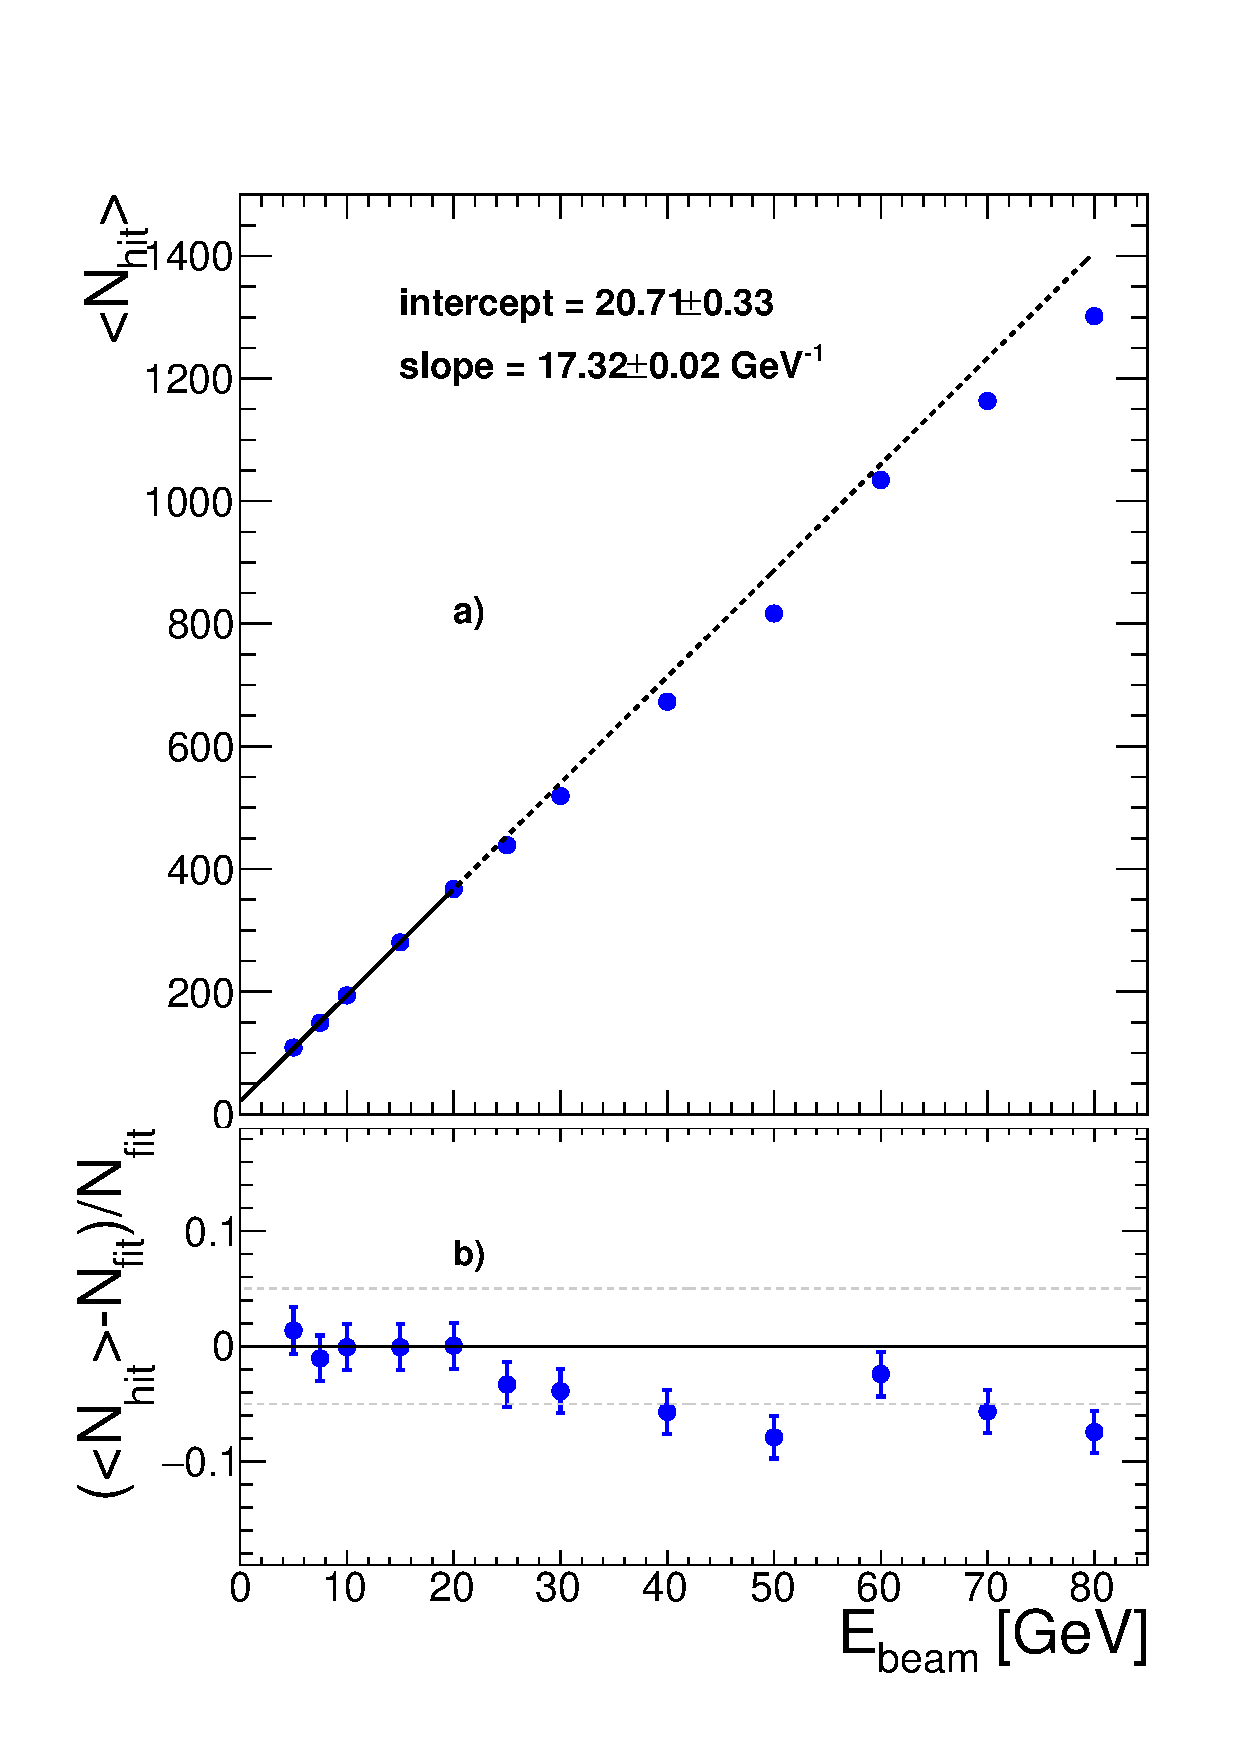
\includegraphics[width=1.2\linewidth]{NHITPION.pdf}
    \end{minipage} \hfill
    \begin{minipage}{0.48\linewidth}
      \begin{center}
        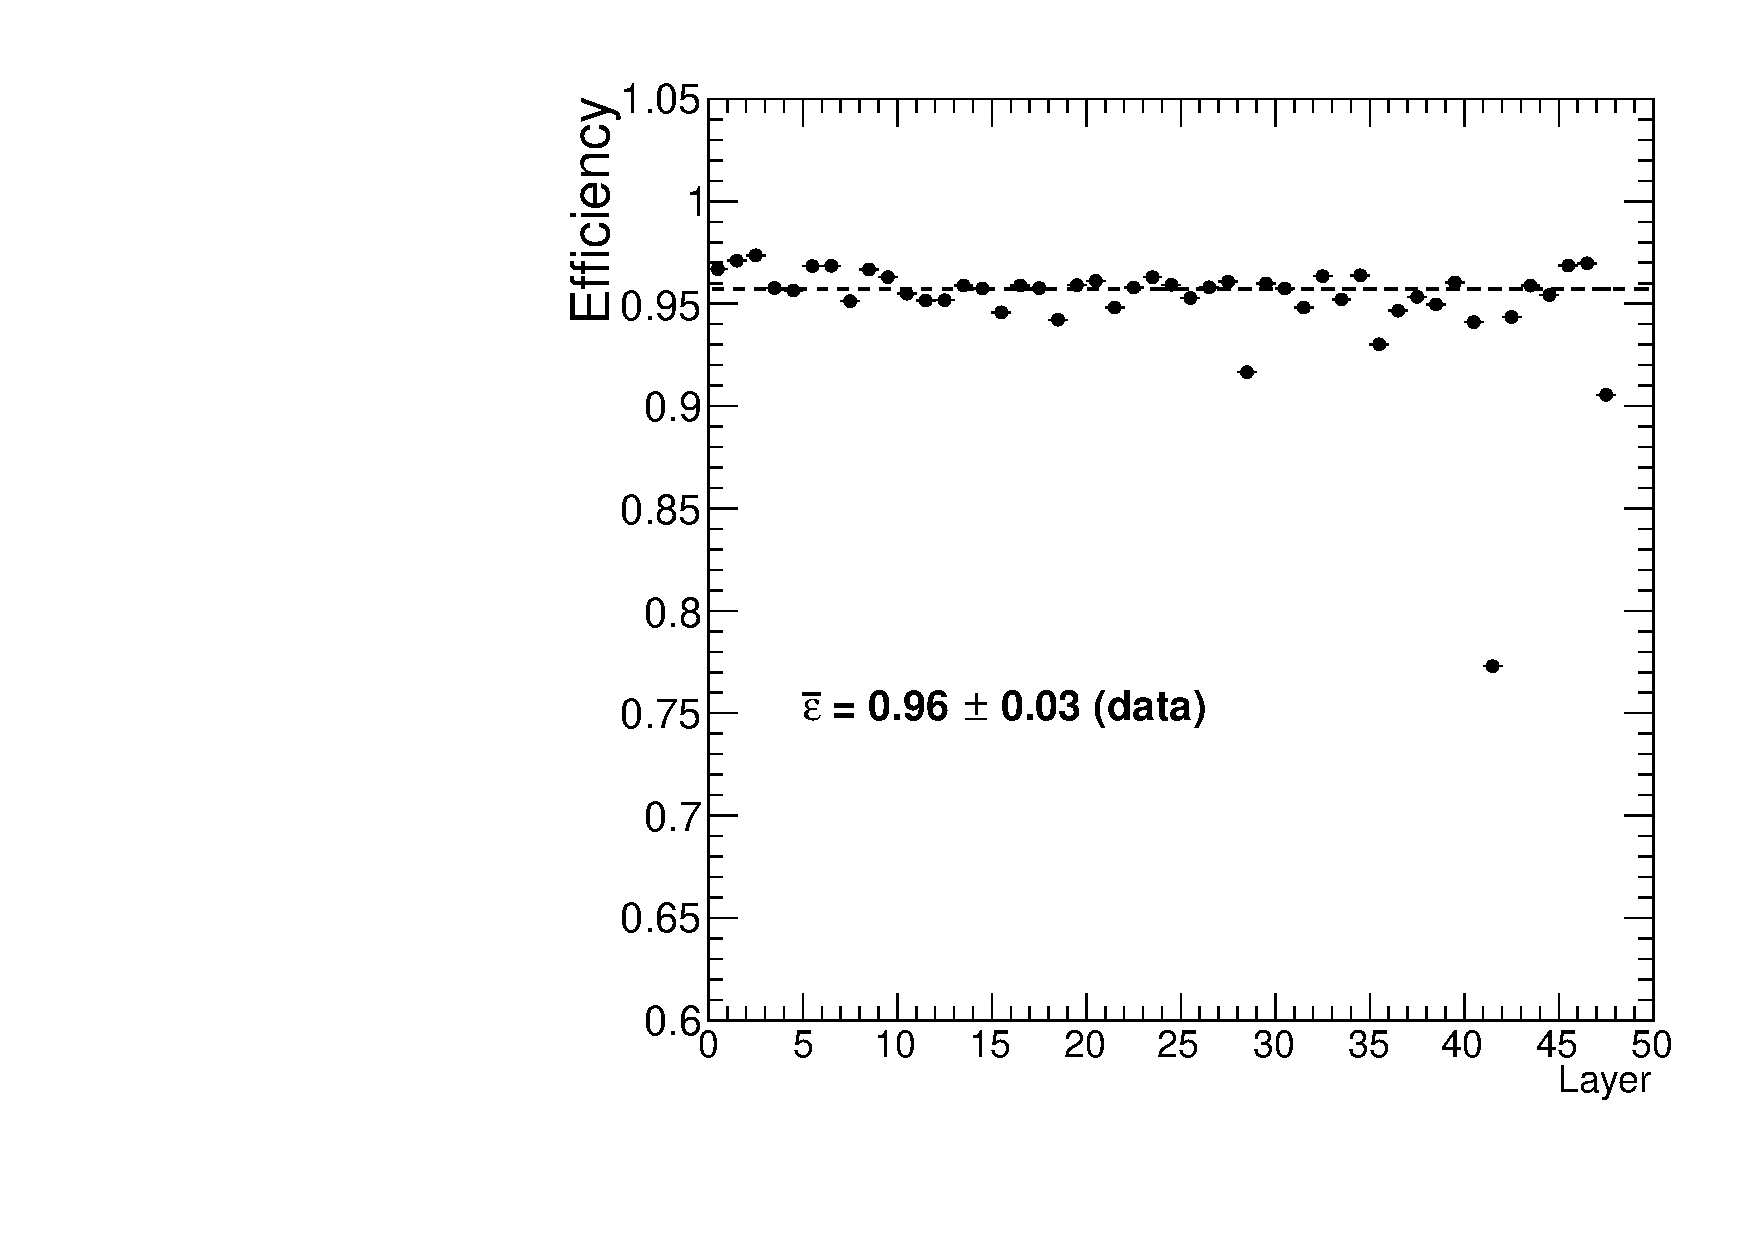
\includegraphics[width=0.7\linewidth]{eff_2012.pdf} \\
        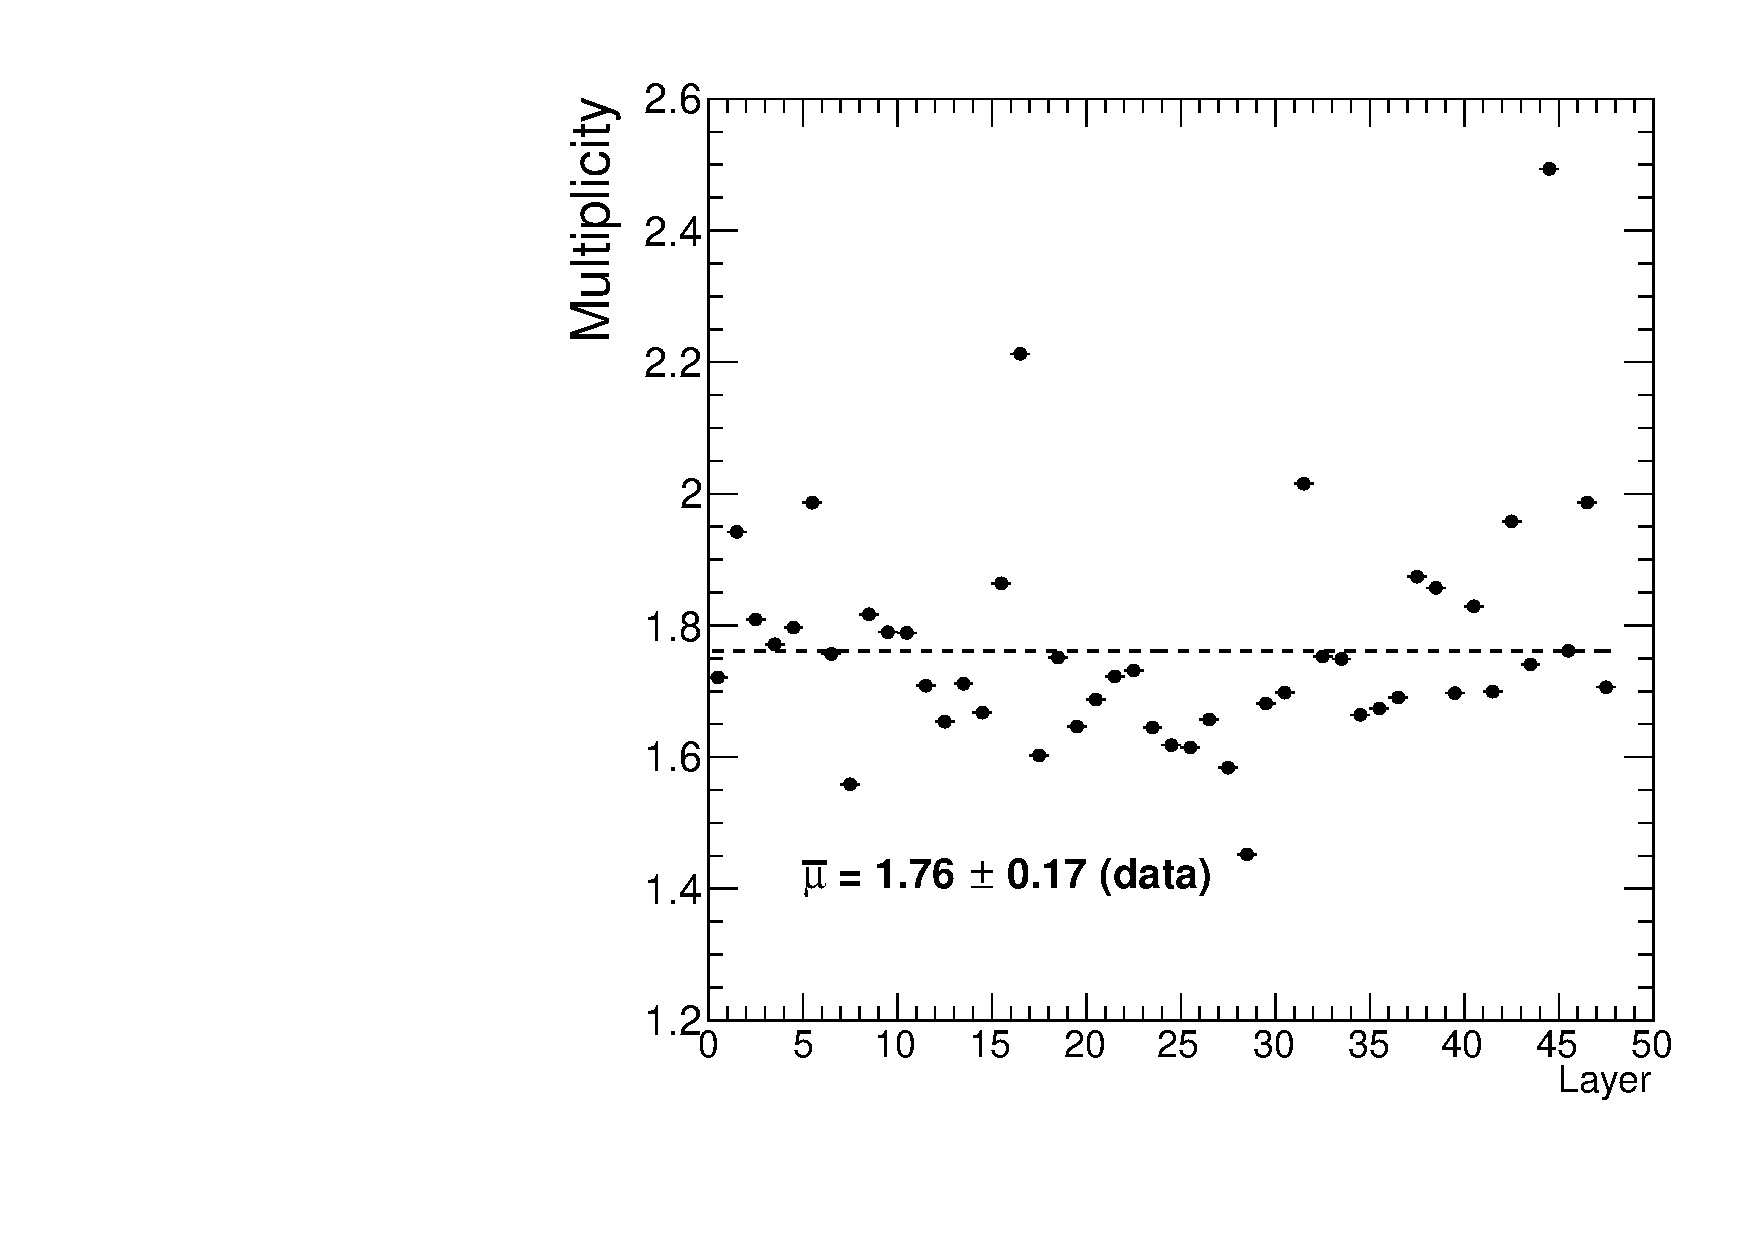
\includegraphics[width=0.7\linewidth]{mul_2012.pdf} \\
        A. Steen [CAN-053. EB]
      \end{center}
    \end{minipage}
  \end{frame}
  
  
  %% Reconstruction de l'énergie
  \begin{frame}
  \frametitle{\secname}
  \framesubtitle{\subsecname}
    \begin{minipage}{0.48\linewidth}
      \begin{block}{Reconstruction de l'énergie}
        {\small
        \begin{equation}
          E = \alpha(NHit)\cdot N_1 + \beta(NHit)\cdot N_2 + \gamma(NHit)\cdot N_3 
        \end{equation}
        avec :
        \begin{equation}
          \alpha(NHit) = \alpha_1 + \alpha_2\cdot NHit + \alpha_3\cdot NHit^2
        \end{equation}
        \begin{equation}
          \beta(NHit) = \beta_1 + \beta_2\cdot NHit + \beta_3\cdot NHit^2
        \end{equation}
        \begin{equation}
          \gamma(NHit) = \gamma_1 + \gamma_2\cdot NHit + \gamma_3\cdot NHit^2
        \end{equation}
        }
      \end{block}
      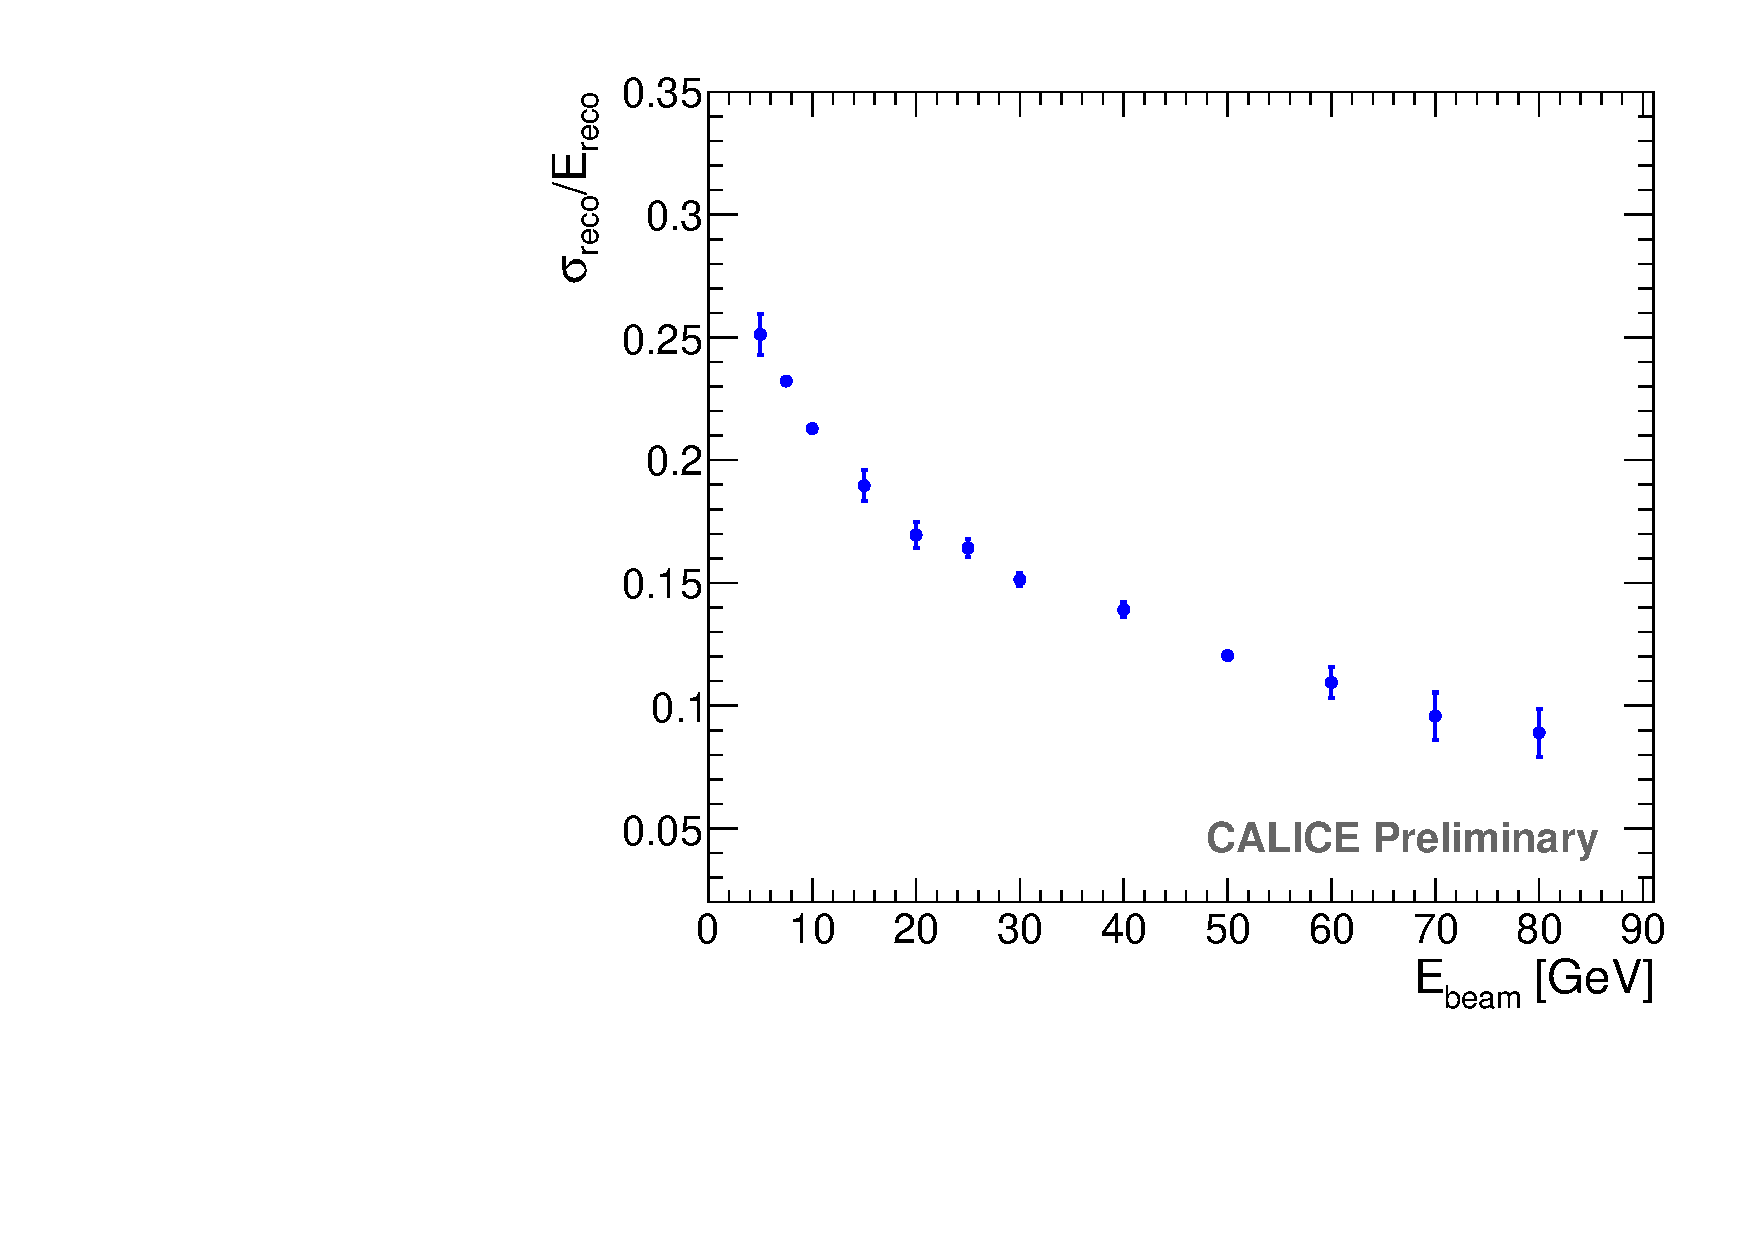
\includegraphics[width=\linewidth]{Energy-Resolution.pdf}
    \end{minipage} \hfill
    \begin{minipage}{0.5\linewidth}
      \begin{center}
        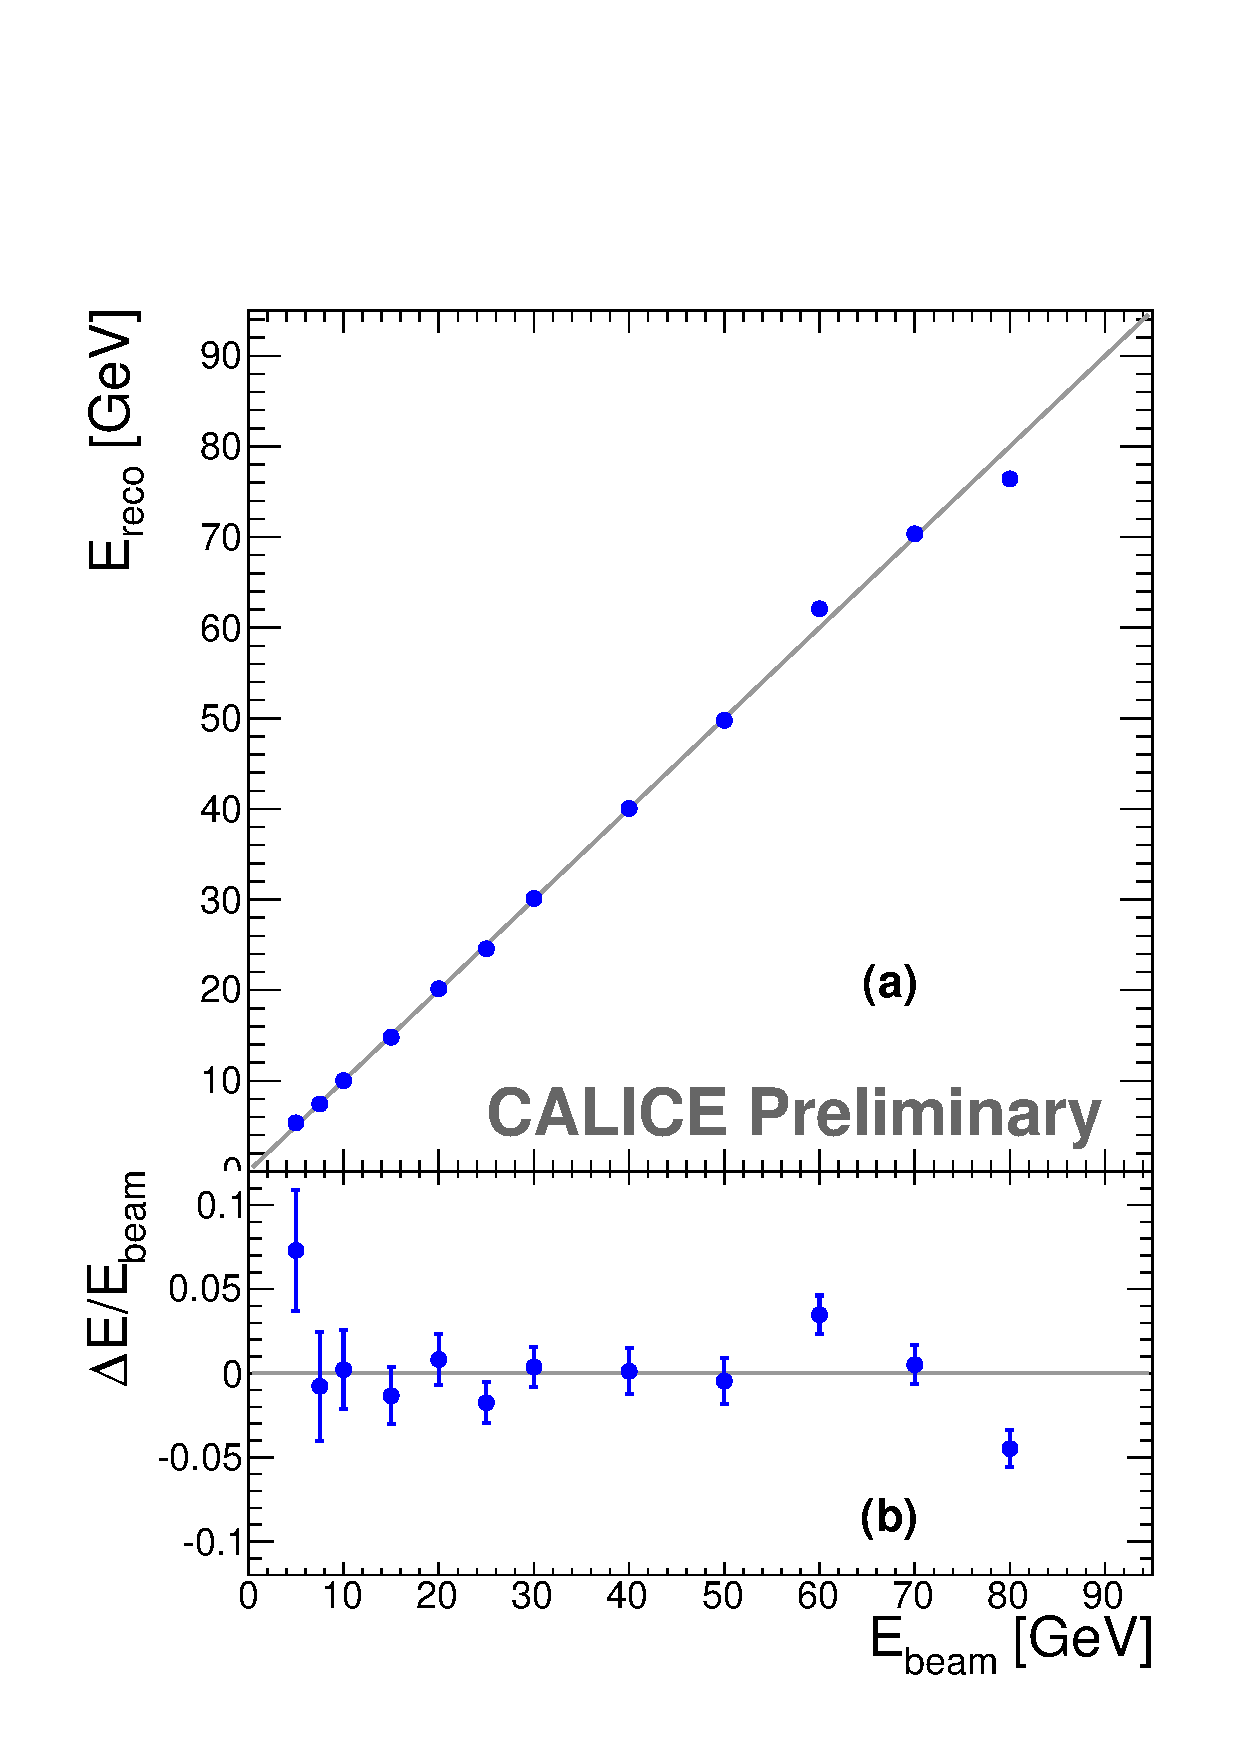
\includegraphics[width=\linewidth]{Energy-Linearity.pdf} \\
        Calice SDHCAL [CAN-037]
      \end{center}
    \end{minipage}
  \end{frame}
  
%%%%%%%%%%%%%%%%%
%% ALGO DE PFA %%
%%%%%%%%%%%%%%%%%
  \section{Algorithme de suivi de particules}
  
  \begin{frame}
  \frametitle{\secname}
    \tableofcontents[currentsection]
  \end{frame}
  
  
  \subsection{Introduction}
  
  %% Généralités du PFA
  \begin{frame}
  \frametitle{\secname}
  \framesubtitle{\subsecname}
    \begin{block}{Définition}
      \textit{\textcolor{red}{Algorithme de reconstruction} visant à reconstruire les particules \textcolor{green}{individuellement} en \textcolor{red}{combinant les informations} les plus appropriées des \textcolor{green}{différents sous-détecteurs}}.
    \end{block}
    \pause
    \begin{center} \textbf{\large PFA = \textcolor{red}{Logiciel} + \textcolor{green}{Détecteur} !!} \end{center}
    \pause
    \begin{minipage}{0.48\linewidth}
      \begin{block}{Sous-détecteurs appropriés}
        \begin{itemize}
          \item $e^{\pm}$ : \textbf{Tracker}
          \item $h^{\pm}$ : \textbf{Tracker}
          \item $\mu^{\pm}$ : \textbf{Tracker} + chambres à muons
          \item $\gamma$ ~~~: \textbf{ECal} + Tracker (track veto)
          \item $h^{0}$ ~: \textbf{ECal + HCal}
        \end{itemize}
      \end{block}
      \begin{block}{Composition moyenne d'un jet de 100 GeV}
        \begin{itemize}
          \item 65 \% particules chargées
          \item 25 \% photons
          \item 10 \% hadrons neutres
        \end{itemize}
      \end{block}
    \end{minipage} \hfill
    \begin{minipage}{0.5\linewidth}
      \begin{center}
        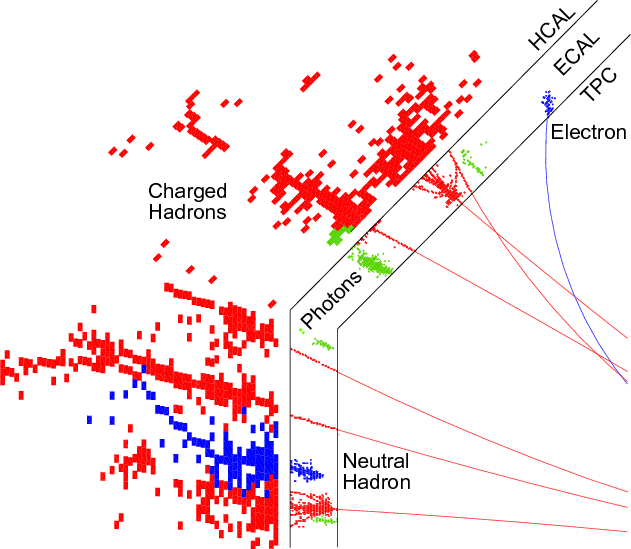
\includegraphics[width=0.95\linewidth]{pfa_event_display.png}
      \end{center}      
    \end{minipage}
  \end{frame}
  
  %% Pandora PFA
  \begin{frame}
  \frametitle{\secname}
  \framesubtitle{\subsecname}
    \begin{minipage}{0.38\linewidth}
      \begin{block}{Pandora PFA}
        \begin{itemize}
          \item Clustering en cone
          \item Associations cluster-cluster, track-cluster
          \item Reclustering statistique
        \end{itemize}
      \end{block}
      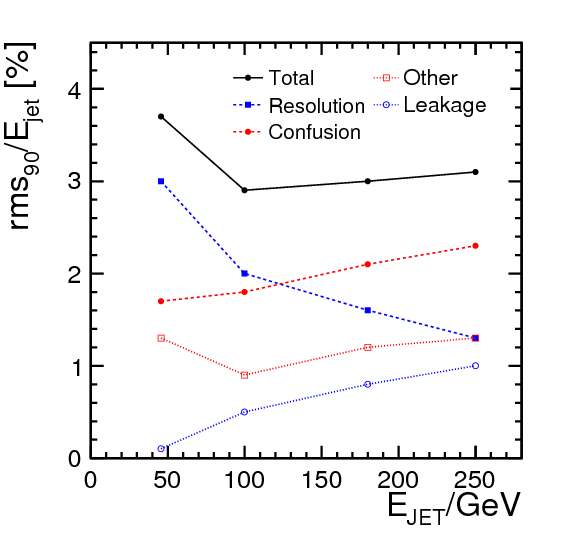
\includegraphics[width=0.9\linewidth]{pandorapfa_jet_energy_resolution.png}
    \end{minipage} ~\hfill
    \begin{minipage}{0.6\linewidth}
      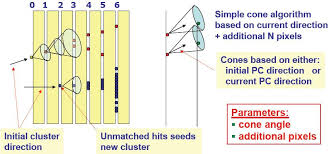
\includegraphics[width=0.9\linewidth]{pandorapfa_cones.jpg} \\
      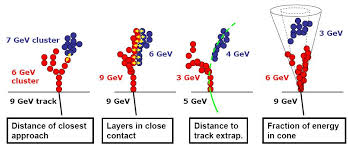
\includegraphics[width=0.9\linewidth]{pandorapfa_associations.jpg}      
    \end{minipage}\pause
    \begin{block}{Mais ...}
      \begin{itemize}
        \item Conçu pour un HCal analogique
        \item Optimisé pour une taille de cellule 3x3$cm^2$
        \item Calcul d'énergie linéaire dans les algorithmes 
      \end{itemize}
    \end{block}
  \end{frame}
  
  %% ArborPFA
  \subsection{ArborPFA}

  %% Principe  
  \begin{frame}
  \frametitle{\secname}
  \framesubtitle{\subsecname - Principe}
    \begin{block}{Principe}
      Algorithme de reconstruction basé sur la \textbf{topologie en arbre} des gerbes hadroniques.
    \end{block}
    \pause
    \begin{minipage}{0.48\linewidth}
      \begin{center}
        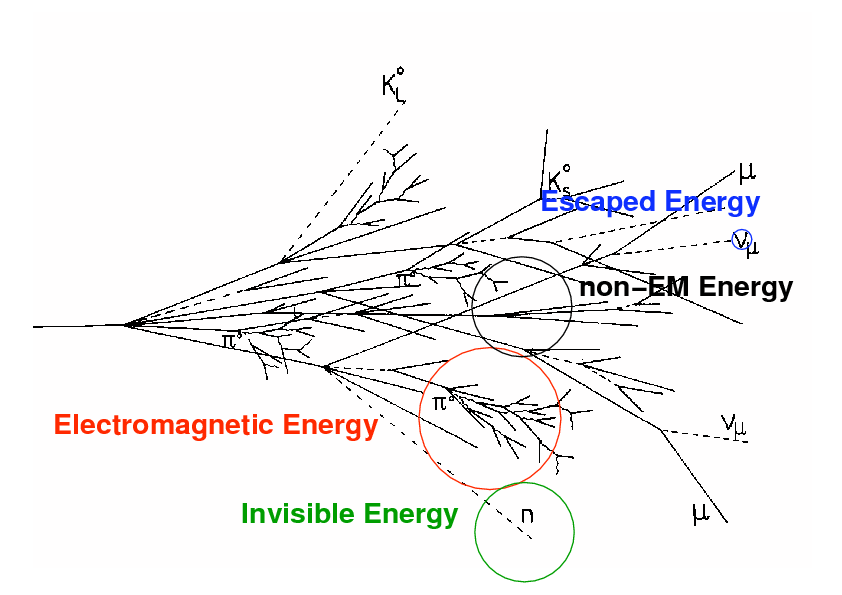
\includegraphics[width=0.8\linewidth]{hadronic_shower.png}      
      \end{center}
    \end{minipage} \hfill
    \begin{minipage}{0.48\linewidth}
      \begin{center}
        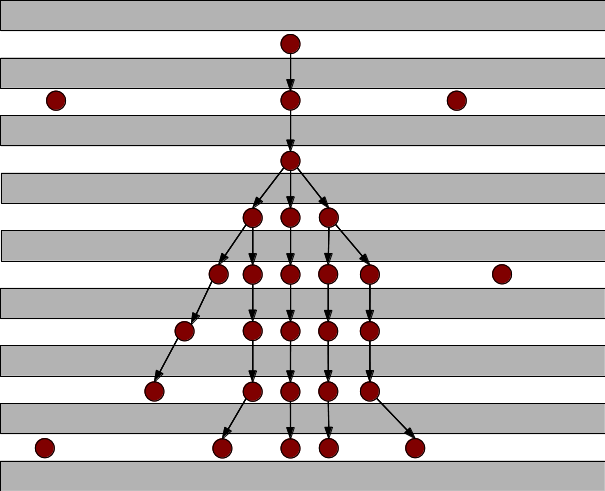
\includegraphics[angle=90, width=0.5\linewidth]{ArborSchema.png}        
      \end{center}
    \end{minipage}
    \pause
    \begin{block}{Quelques definitions}
      \begin{itemize}
        \item \textbf{Objet} : \textit{Noeud} relié par un ou plusieurs connecteurs (+ objets racines et feuilles)
        \item \textbf{Connecteur} : \textit{Lien} orienté liant deux objets
        \item \textbf{Direction de flux} : Orientation du connecteur, vers l'avant ou l'arrière
        \item \textbf{Arbre} : Ensemble d'objets reliés par des connecteurs. Pour chaque objet :
        \begin{itemize}
          \item 0 ou 1 connecteur vers l'arrière
          \item 0 ou plusieurs connecteurs vers l'avant
        \end{itemize}
        $\rightarrow$ Implique une solution d'arbre unique
      \end{itemize}
    \end{block}
  \end{frame}
  
  
  %% Description des algos 1
  \begin{frame}
  \frametitle{\secname}
  \framesubtitle{\subsecname - Les algorithmes}
    \begin{minipage}{0.48\linewidth}
      \begin{block}{\textcircled{{\small 1}} Création d'objects}
        $\blacksquare$ Créé des objets, prêt à être connecter
        \begin{itemize}
          \item Clustering PV dans chaque plan
          \item Si taille du cluster <= 4, cluster = 1 objet
          \item Si taille du cluster > 4, chaque hit du cluster = 1 objet 
        \end{itemize}
        Permet de :
        \begin{itemize}
          \item s'affranchir de la multiplicité dans le SDHCAL
          \item réduire la taille du problème \\ NHit $\rightarrow$ NObject (< NHit)
          \item accélérer le traitement des connexions
        \end{itemize}
      \end{block}
    \end{minipage} \hfill
    \begin{minipage}{0.48\linewidth}
      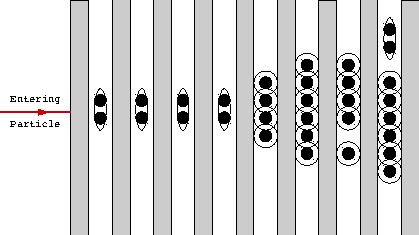
\includegraphics[width=0.9\linewidth]{ObjectCreationAfter.pdf} \\
%       \pause
%       \begin{block}{\textcircled{{\small 2}} Étiquetage des objets de segments de traces}
%         $\blacksquare$ Identifie les objets appartenant aux segments de traces avec des critères d'isolation et étiquette ces objets.
%       \end{block}
    \end{minipage}
  \end{frame}
  
  
  %% Description des algos 2
  \begin{frame}
  \frametitle{\secname}
  \framesubtitle{\subsecname - Les algorithmes}
    \begin{block}{Construction des arbres}
      Phase d’itération :
      \begin{itemize}
        \item Création de connecteurs entre objets (seeding)
        \item Nettoyage des connecteurs pour obtenir une structure en arbre (cleaning)
      \end{itemize}
      \underline{Idée générale} : créer une première structure en arbre globale puis altérer cette structure en créant d'autre connexions plus optimisées.
    \end{block}
%     \pause
%     \begin{minipage}{0.49\linewidth}
%       \begin{block}{\textcircled{{\small 3}} Connexion du segment de trace primaire}
%         $\blacksquare$ Algorithme visant à créer les connections entre objets appartenant au segment de trace primaire. \\
%         Utilise le point d'entrée de la trace chargée et connecte uniquement les objets étiqueté par l'algorithme \textcircled{{\small 2}}. \\
%       \end{block}
%     \end{minipage} \hfill
%     \begin{minipage}{0.49\linewidth}
%       \begin{center}
%         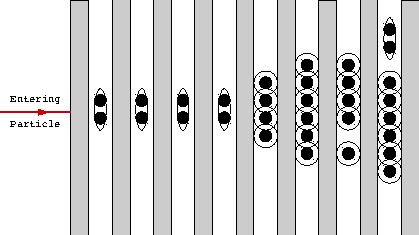
\includegraphics[width=\linewidth]{ObjectCreationAfter.pdf}        
%       \end{center}
%     \end{minipage}
  \end{frame}
  
  
  %% Description des algos 3
  \begin{frame}
  \frametitle{\secname}
  \framesubtitle{\subsecname - Les algorithmes}
%     \begin{minipage}{0.55\linewidth}
      \begin{block}{\textcircled{{\small 2}} Création des connecteurs 1}
        $\blacksquare$ Pour chaque objet, on cherche les objets proches dans les 3 plans suivants à une distance maximale de 45 mm et on créer une connexion pour chacun d'entre eux.
      \end{block}
%       \begin{block}{\textcircled{{\small 5}} Nettoyage des connecteurs 1}
%         $\blacksquare$ Pour chaque objet, on définit un vecteur de référence vers l'arrière :
%         \begin{equation}
%           \vec{C}_{ref} = w_{bck} . \sum_\sigma \sum_b \vec{c}_{b,\sigma} - w_{fwd} . \sum_\delta \sum_f \vec{c}_{f,\delta}
%         \end{equation}
%         On définit aussi le paramètre d'ordre $\kappa$ :
%         \begin{equation}
%           \kappa~=~\Big(\frac{\theta}{\pi}\Big)^{p_{\theta}} . ~\Big(\frac{\Delta}{\Delta_{max}}\Big)^{p_{\Delta}} 
%         \end{equation}
%         Le connecteur vers l'arrière avec le \textbf{paramètre $\kappa$ minimal} est gardé. Une fois le connecteur arrières de chaque objet identifié, on supprime tous les autres connecteurs. \\
%         $\rightarrow$ Première structure en arbre !
%       \end{block}
%     \end{minipage} \hfill
%     \begin{minipage}{0.44\linewidth}
      \begin{center}
        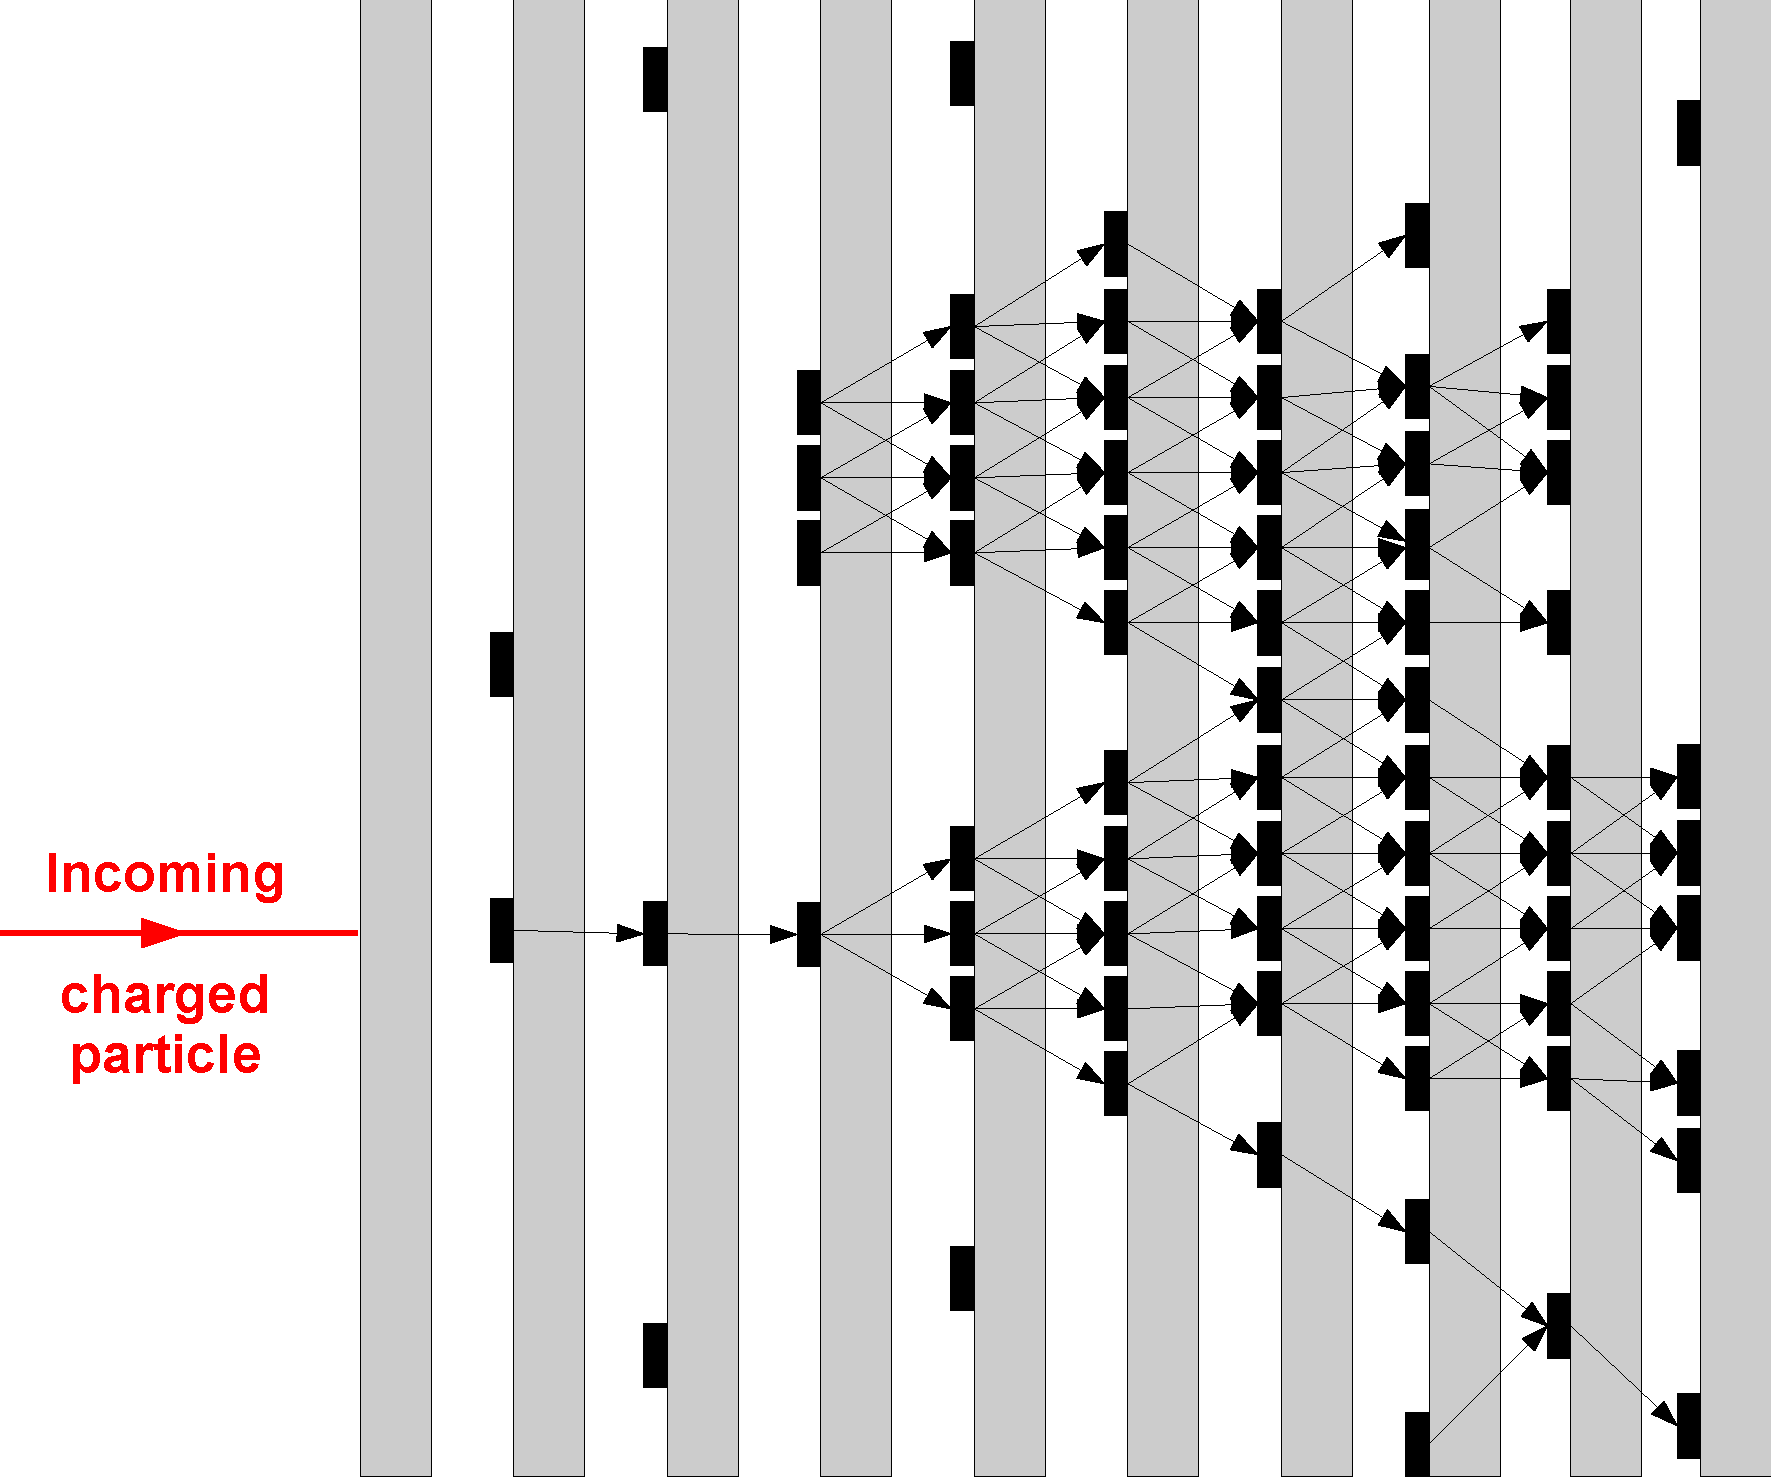
\includegraphics[width=0.6\linewidth]{ConnectorSeeding1.pdf} \\ ~ \\
      \end{center}
%     \end{minipage}
  \end{frame}
  
  
    %% Description des algos 3
  \begin{frame}
  \frametitle{\secname}
  \framesubtitle{\subsecname - Les algorithmes}
    \begin{minipage}{0.55\linewidth}
      \begin{block}{\textcircled{{\small 3}} Nettoyage des connecteurs 1}
        \onslide<1->{$\blacksquare$ Nettoyage des connecteurs pour former une structure en arbre.} \\
        \onslide<2->{Pour chaque objet :}
        \begin{itemize}
          \item<3-> Calcul de la direction de référence :
          \begin{equation}
            \vec{C}_{ref} = w_{bck} . \sum_\sigma \sum_b \vec{c}_{b,\sigma} - w_{fwd} . \sum_\delta \sum_f \vec{c}_{f,\delta}
          \end{equation}
          \item<4-> Pour chaque objet connecté en arrière, on définit le paramètre d'ordre $\kappa$ :
          \begin{equation}
            \kappa~=~\Big(\frac{\theta}{\pi}\Big)^{p_{\theta}} . ~\Big(\frac{\Delta}{\Delta_{max}}\Big)^{p_{\Delta}} 
          \end{equation}
          \item<5-> Le connecteur vers l'arrière avec le \textbf{paramètre $\kappa$ minimal} est gardé. 
          \item<6-> \textbf{A la fin de l'algorithme}, on supprime tous les autres connecteurs. \\
        \end{itemize}
        \onslide<7->{$\rightarrow$ On obtient une structure en arbre.}
      \end{block}
    \end{minipage} \hfill
    \begin{minipage}{0.3\linewidth}
      \begin{center}
        \begin{overlayarea}{\linewidth}{\linewidth}
          \includegraphics[width=1.1\linewidth]<-2>{ConnectorCleaningExample1.pdf}
          \includegraphics[width=1.1\linewidth]<3>{ConnectorCleaningExample2.pdf}
          \includegraphics[width=1.1\linewidth]<4>{ConnectorCleaningExample3.pdf}
          \includegraphics[width=1.1\linewidth]<5>{ConnectorCleaningExample4.pdf}
          \includegraphics[width=1.1\linewidth]<6->{ConnectorCleaningExample5.pdf}      
        \end{overlayarea}
      \end{center}
    \end{minipage}
  \end{frame}
  
  %% Description des algos 4
  \begin{frame}
  \frametitle{\secname}
  \framesubtitle{\subsecname - Les algorithmes}
    \begin{block}{\textcircled{{\small 4}} et \textcircled{{\small 5}} Alignement des connexions}
      $\blacksquare$ A partir de la structure en arbre déjà existante, d'autre connexions sont créés pour aligner les connecteurs dans l'arbre. Un second nettoyage est effectué pour finalement obtenir une structure en arbre.
    \end{block}
    \begin{center}
      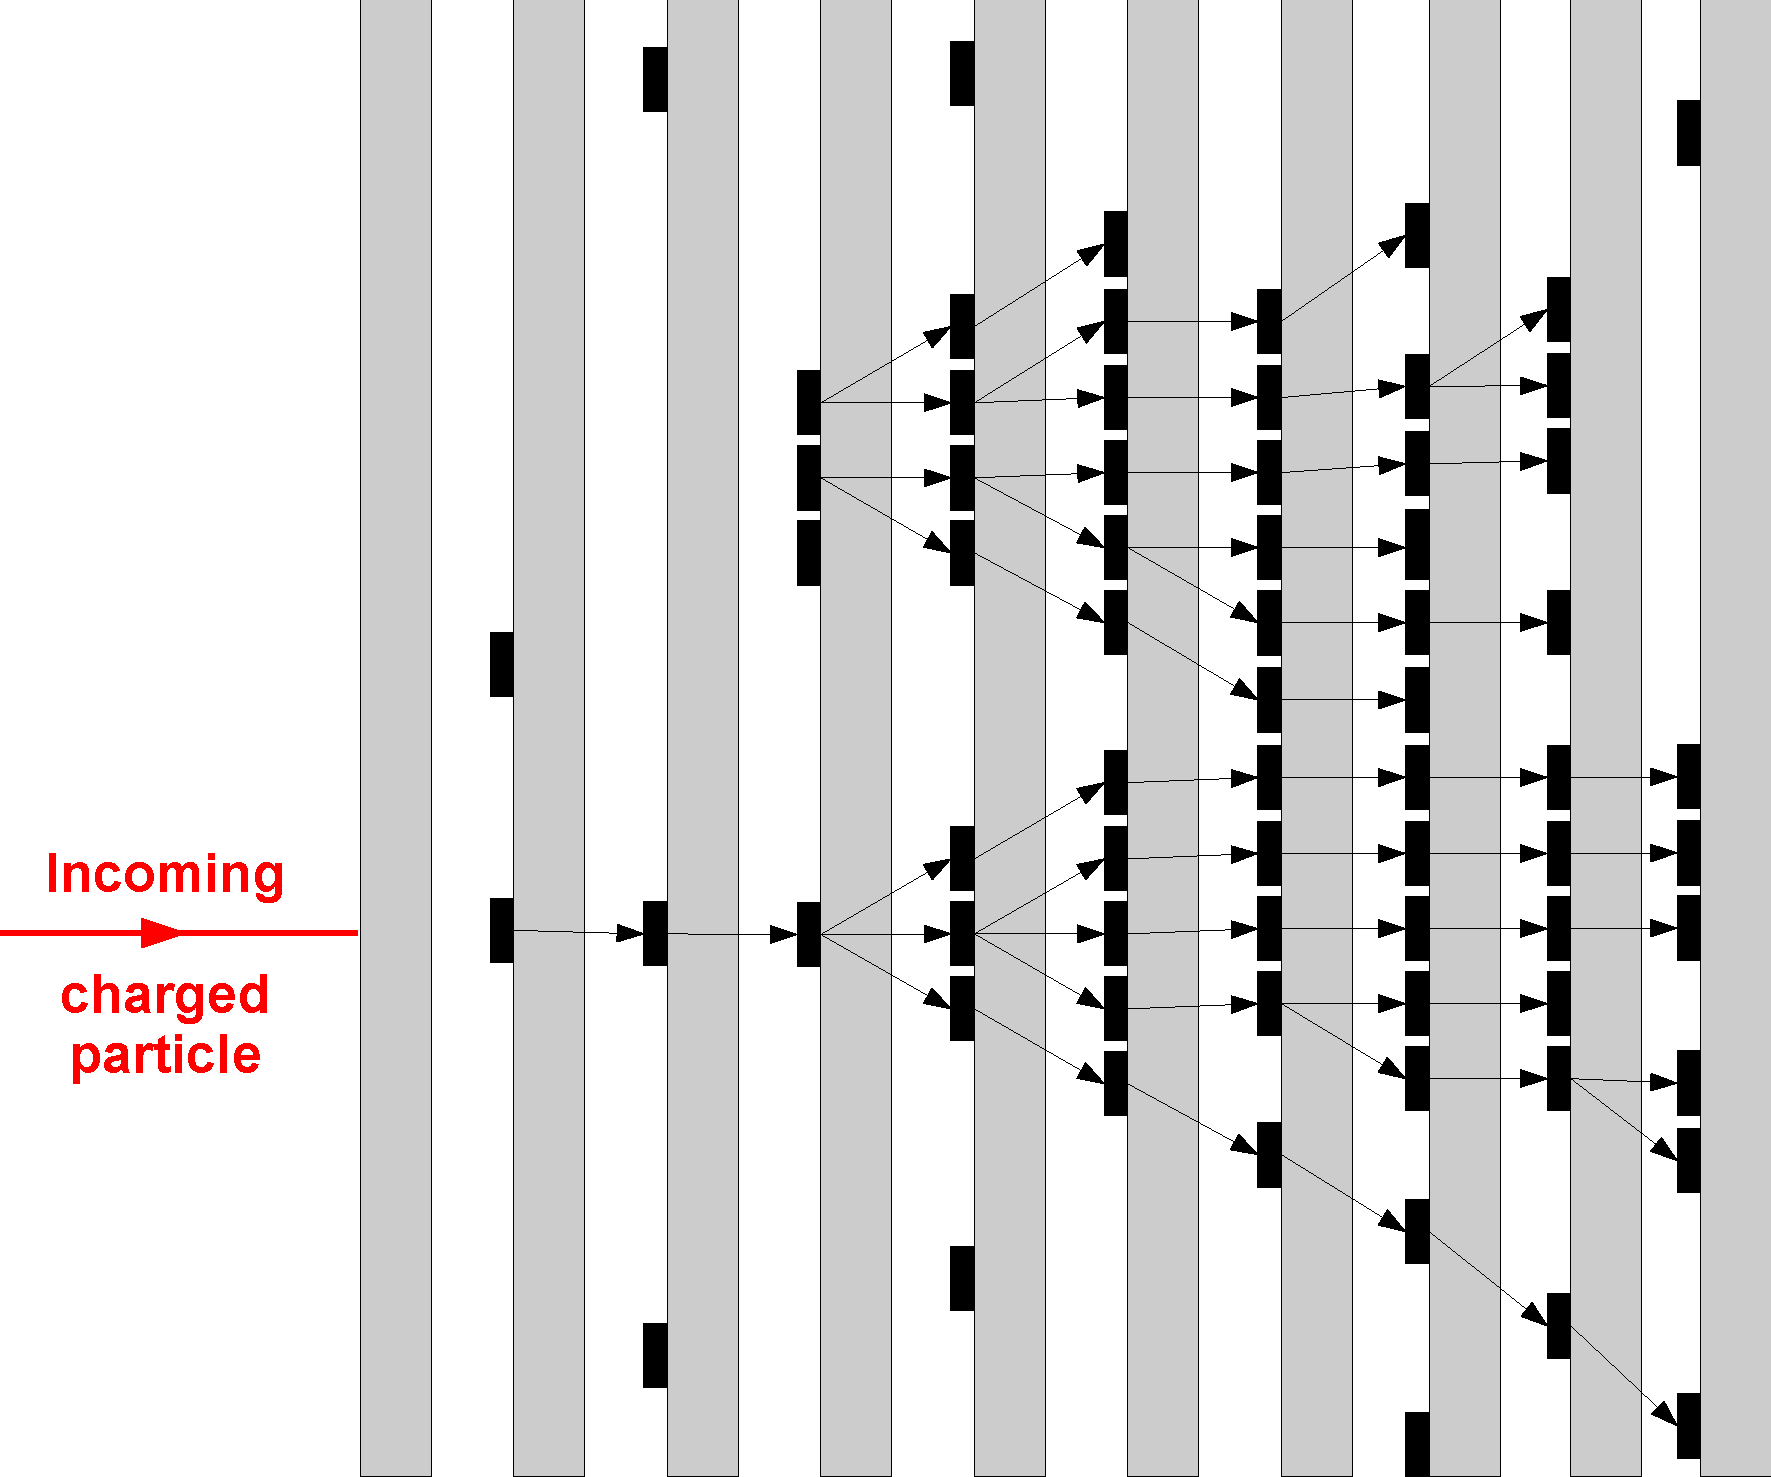
\includegraphics[width=0.6\linewidth]{ConnectorCleaning2.pdf}      
    \end{center}
  \end{frame}
  
  %% Description des algos 5
  \begin{frame}
  \frametitle{\secname}
  \framesubtitle{\subsecname - Les algorithmes}
    \begin{minipage}{0.55\linewidth}
      \begin{block}{\textcircled{{\small 6}} Association trace - arbre}
        $\blacksquare$ Association entre les traces et les arbres en fonction de critères simples :
        \begin{itemize}
          \item Distance entre les racines des arbres et l'extrapolation de la trace au calorimètre
          \item Comparaison impulsion - énergie de l'arbre
          \item Prise en compte des cas d'interactions tôt dans le calorimètre
        \end{itemize}
      \end{block}
      \begin{block}{\textcircled{{\small 7}} Fusion des arbres neutres}
        $\blacksquare$ Interaction des particules neutres dans un absorbeur \\
        $\rightarrow$ Plusieurs racines dans un même plan et donc plusieurs arbres reconstruits au lieu d'un seul. \\
        Les racines appartenant à ce type de configuration sont \textbf{identifiés} et les arbres \textbf{fusionnés}.  
      \end{block}
    \end{minipage} \hfill
    \begin{minipage}{0.44\linewidth}
      \begin{center}
        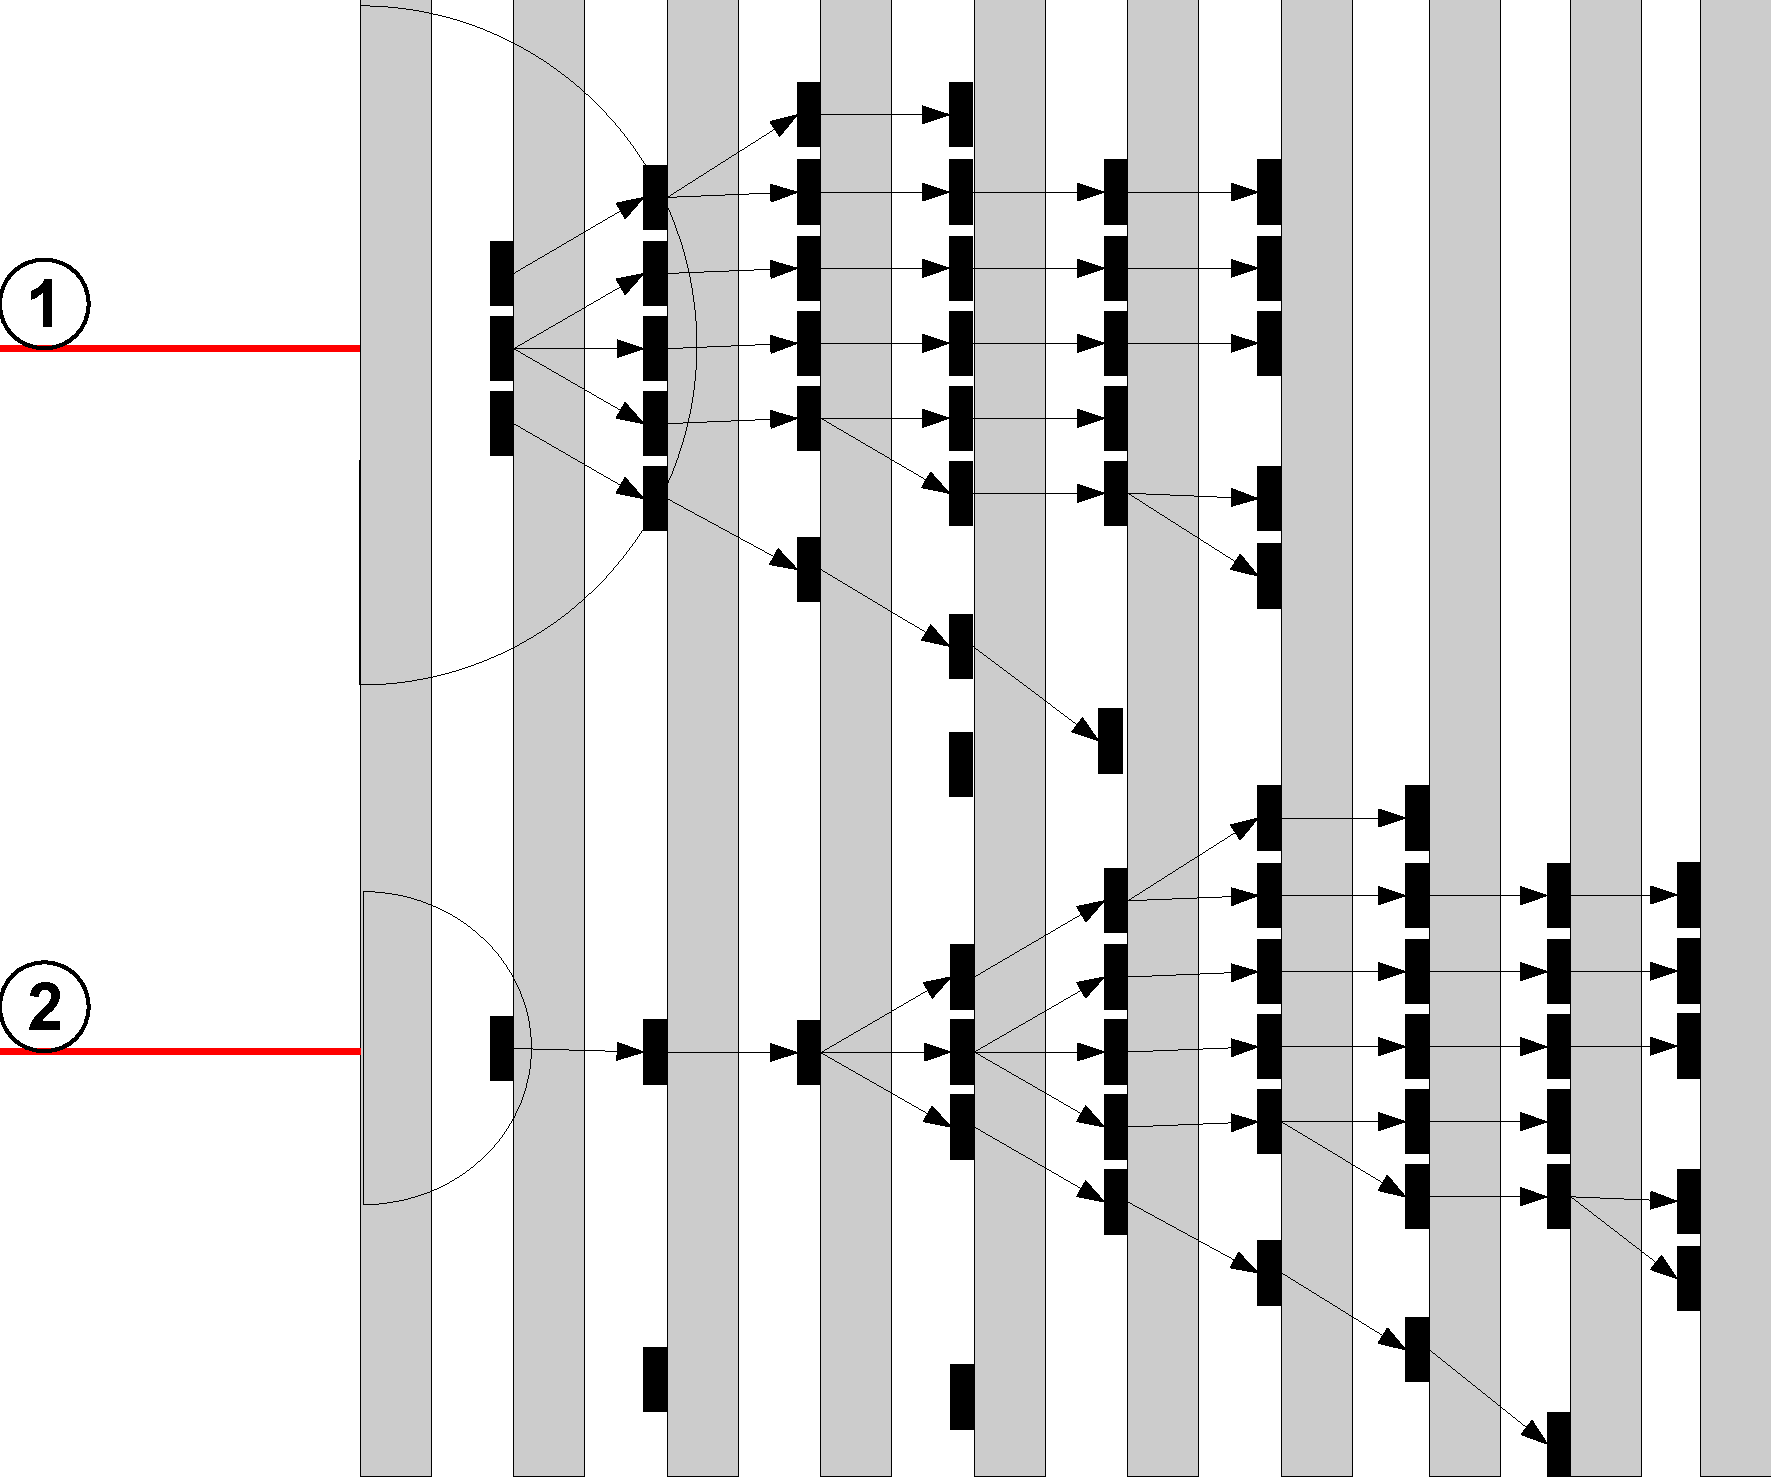
\includegraphics[width=0.9\linewidth]{EnergyDrivenTrackClusterAssociation.pdf} \\
        ~ \\
        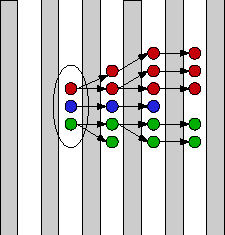
\includegraphics[width=0.5\linewidth]{NeutralTreeMerging.pdf}
      \end{center}
    \end{minipage}
  \end{frame}
  

  %% Description des algos 6
  \begin{frame}
  \frametitle{\secname}
  \framesubtitle{\subsecname - Les algorithmes}
    \begin{minipage}{0.55\linewidth}
      \begin{block}{\textcircled{{\footnotesize 8}} Association d'arbres pointant sur d'autres}
        $\blacksquare$ Association d'arbres neutres (fils) à des arbres neutres ou chargés (parent) en fonction de leurs axes principaux (ajustement linéaire 3D sur la position des objets) et de leurs énergies.
        \begin{itemize}
          \item Croisement proche axe-axe
          \item Croisement proche axe-barycentre
          \item Critères d'énergies
        \end{itemize}
      \end{block}
      \begin{block}{\textcircled{{\footnotesize 9}} Fusion des petits arbres neutres}
        $\blacksquare$ Les arbres de petite taille (NObj < 20) sont fusionnés dans l'arbre le plus proche de grande taille
      \end{block}
    \end{minipage} \hfill
    \begin{minipage}{0.415\linewidth}
      \begin{center}
        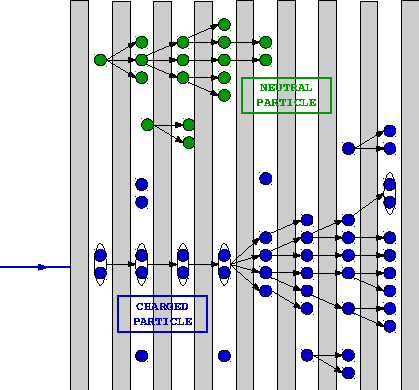
\includegraphics[width=\linewidth]{PfoCreation.pdf}
      \end{center}
      \begin{block}{\textcircled{{\footnotesize 10}} Création de \textit{Particle Flow Objects}}
        $\blacksquare$ Création de particules reconstruites :
        \begin{itemize}
          \item une trace (si chargé)
          \item un arbre
        \end{itemize}
      \end{block} 
    \end{minipage}
  \end{frame}
  
  %% Performance ArborPFA - single particle
  \subsection{Performance - Hadron seul}
  \begin{frame}
  \frametitle{\secname}
  \framesubtitle{\subsecname}
    \begin{minipage}{0.56\linewidth}
      \begin{block}{Données d'entrée du programme de reconstruction}
        \begin{itemize}
          \item Données : CERN SPS 2012 - Août-Septembre \\
          \item Particules : $h^{\pm}$
          \item Énergies : [10 ; 80] GeV par pas de 10 GeV
          \item "Fausse" trace générée : 
          \begin{itemize}
            \item $\vec{p}$ = (0, 0, $E_{beam}$)
            \item Point d'entré $\vec{e}$ : barycentre ($b_x$, $b_y$) des hits dans les 5 premiers plans \\
            $\rightarrow$ $\vec{e}$ = (b$_x$, b$_y$, z$_{front}$)
          \end{itemize}
          \item Pas de champs magnétique ($\vec{B}$ = $\vec{0}$ T)
        \end{itemize}
      \end{block}
    \end{minipage} \hfill
    \begin{minipage}{0.43\linewidth}
      \begin{center}
        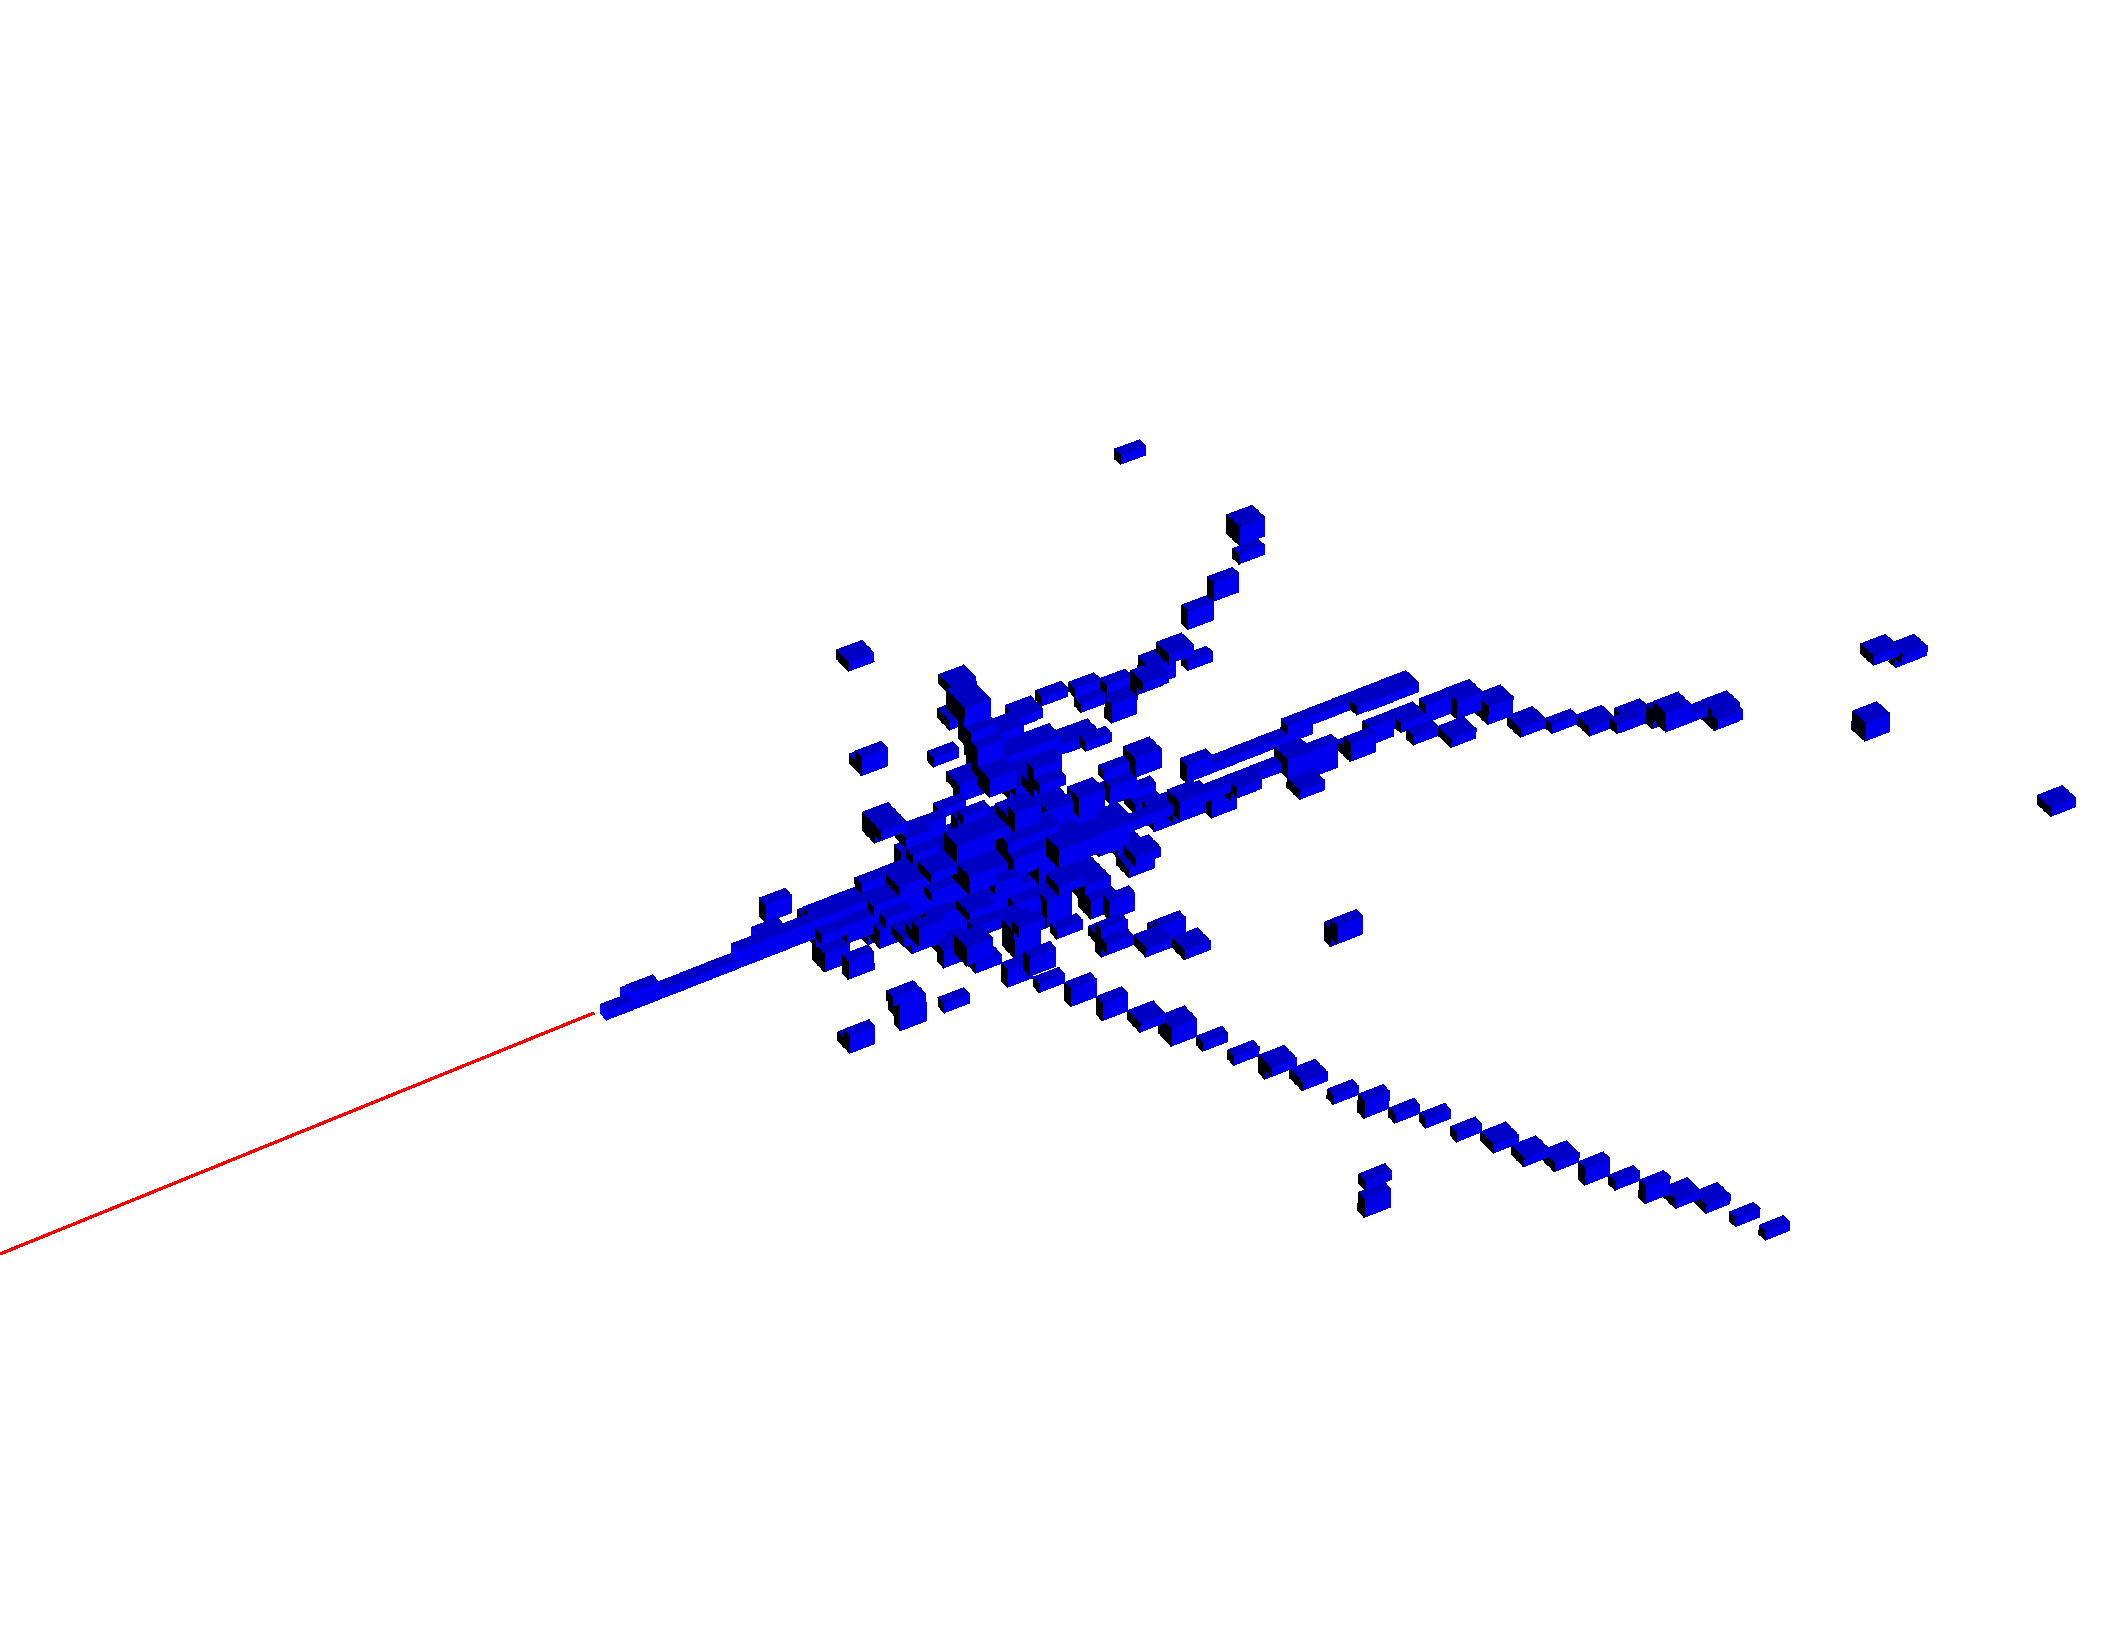
\includegraphics[width=0.9\linewidth]{SingleParticleSetup.pdf}      
      \end{center}
    \end{minipage}
  \end{frame}
  
  
  %% Performance ArborPFA - single particle - plots
  \begin{frame}
  \frametitle{\secname}
  \framesubtitle{\subsecname}
    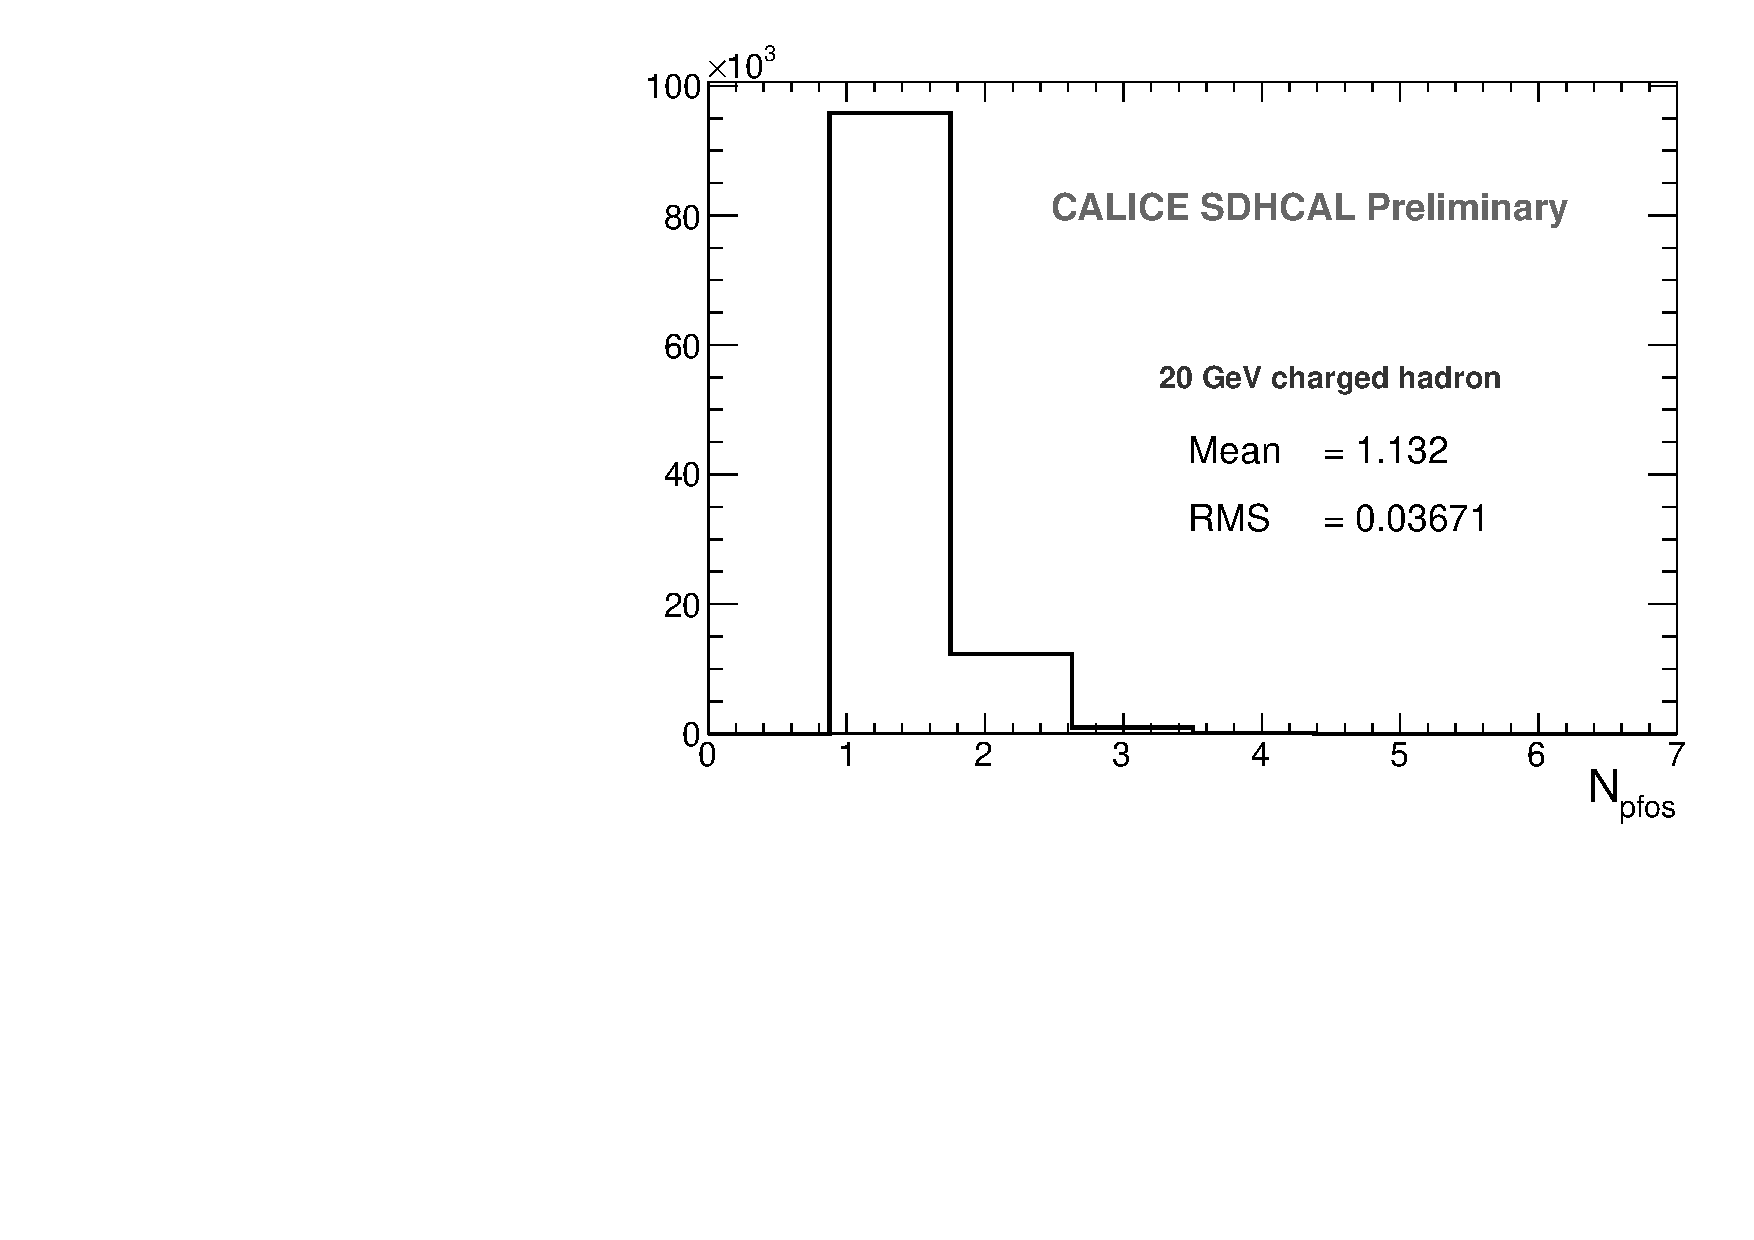
\includegraphics[width=0.45\linewidth]{SingleParticle_NPfos_20GeV.pdf}~
    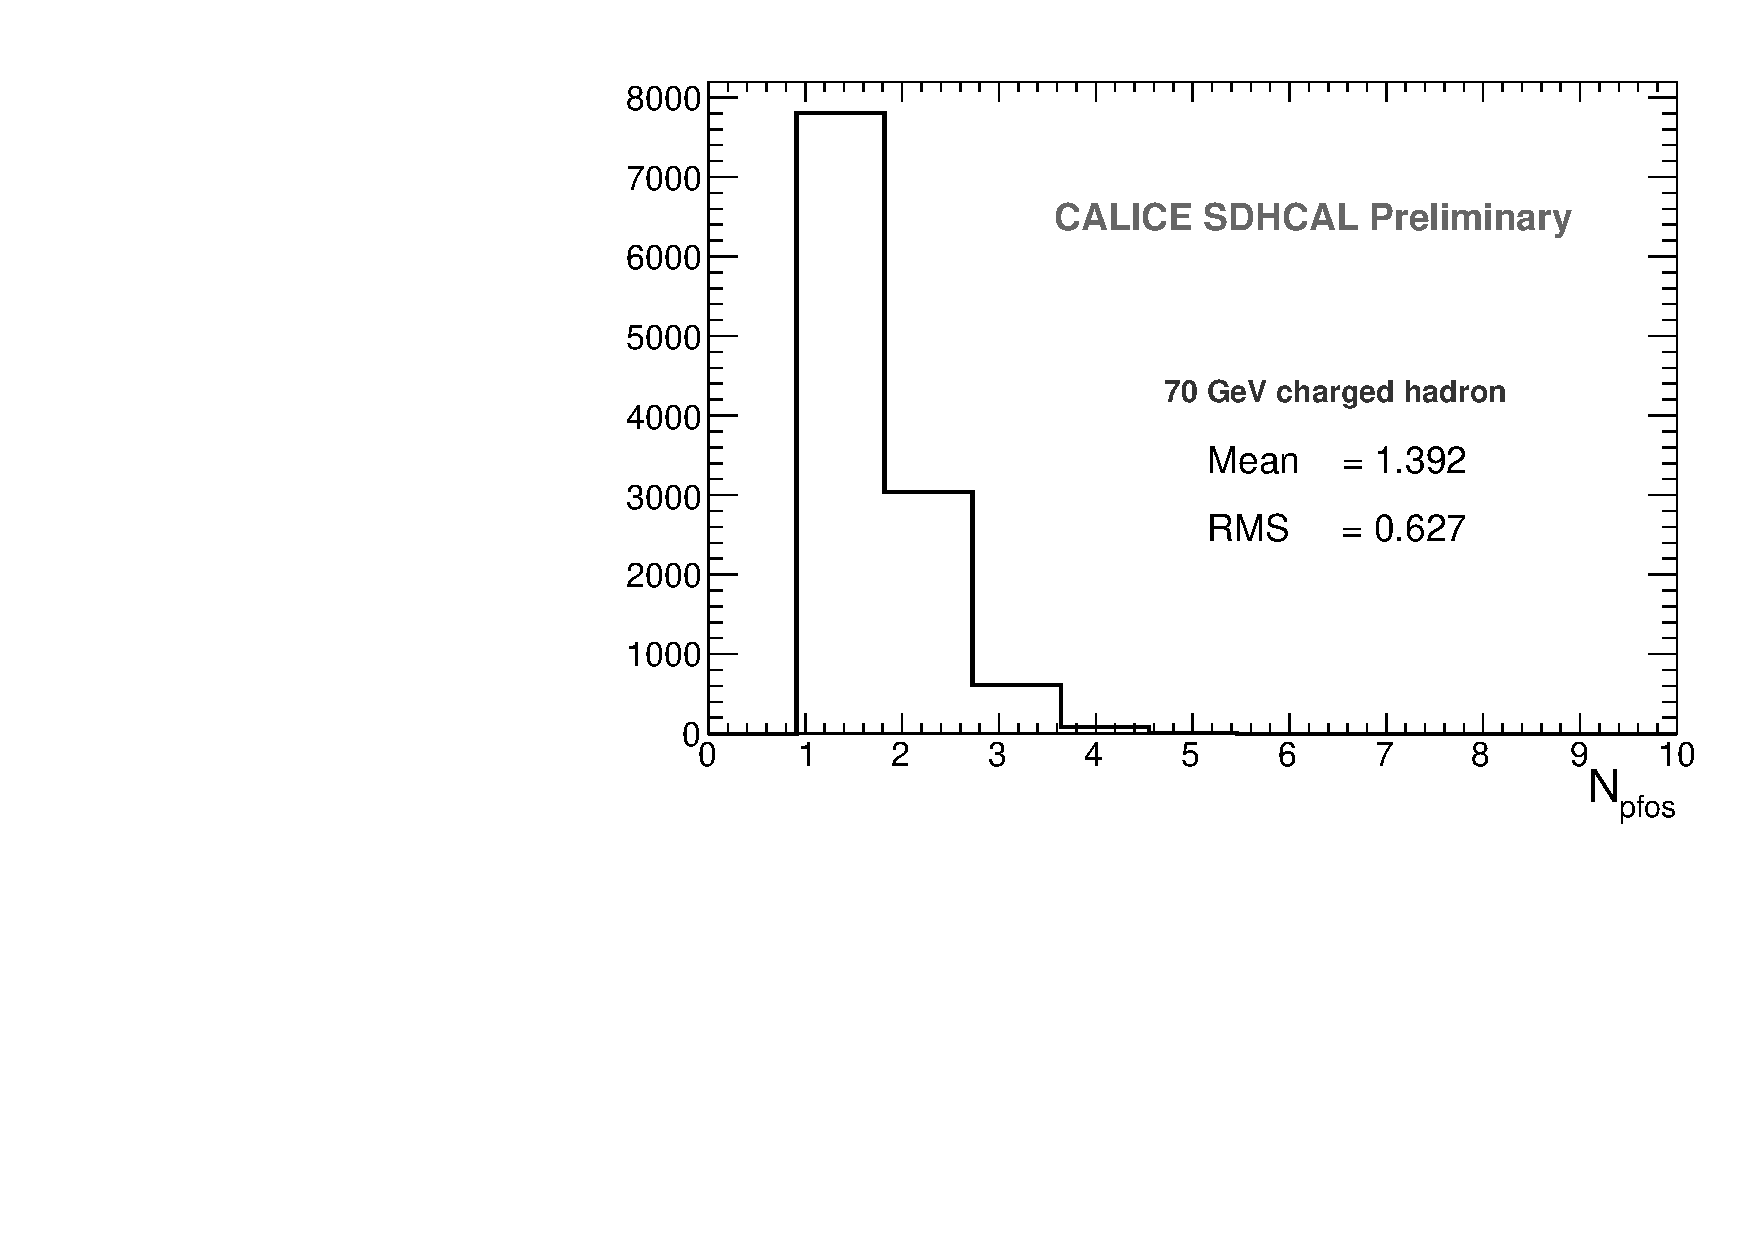
\includegraphics[width=0.45\linewidth]{SingleParticle_NPfos_70GeV.pdf} \\
    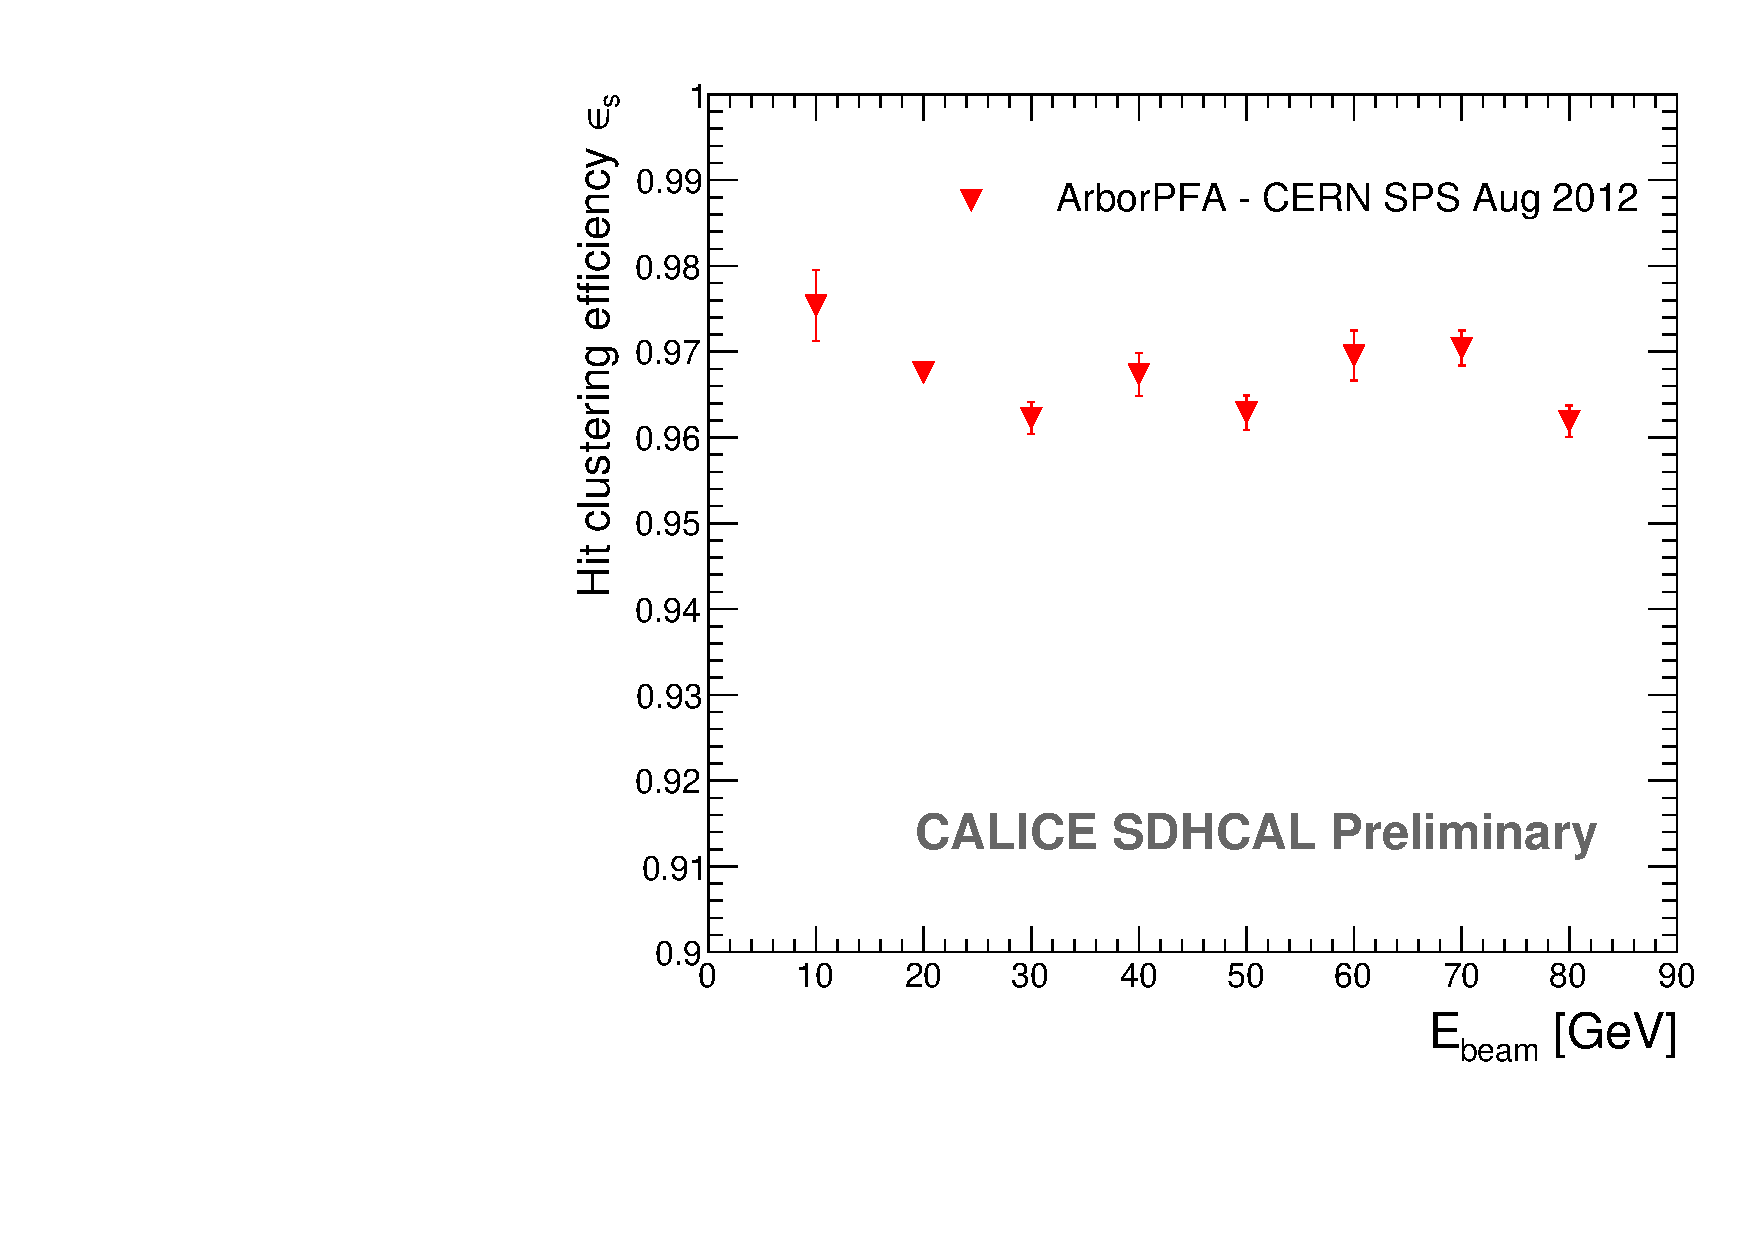
\includegraphics[width=0.45\linewidth]{SingleParticle_Efficiency.pdf}~
    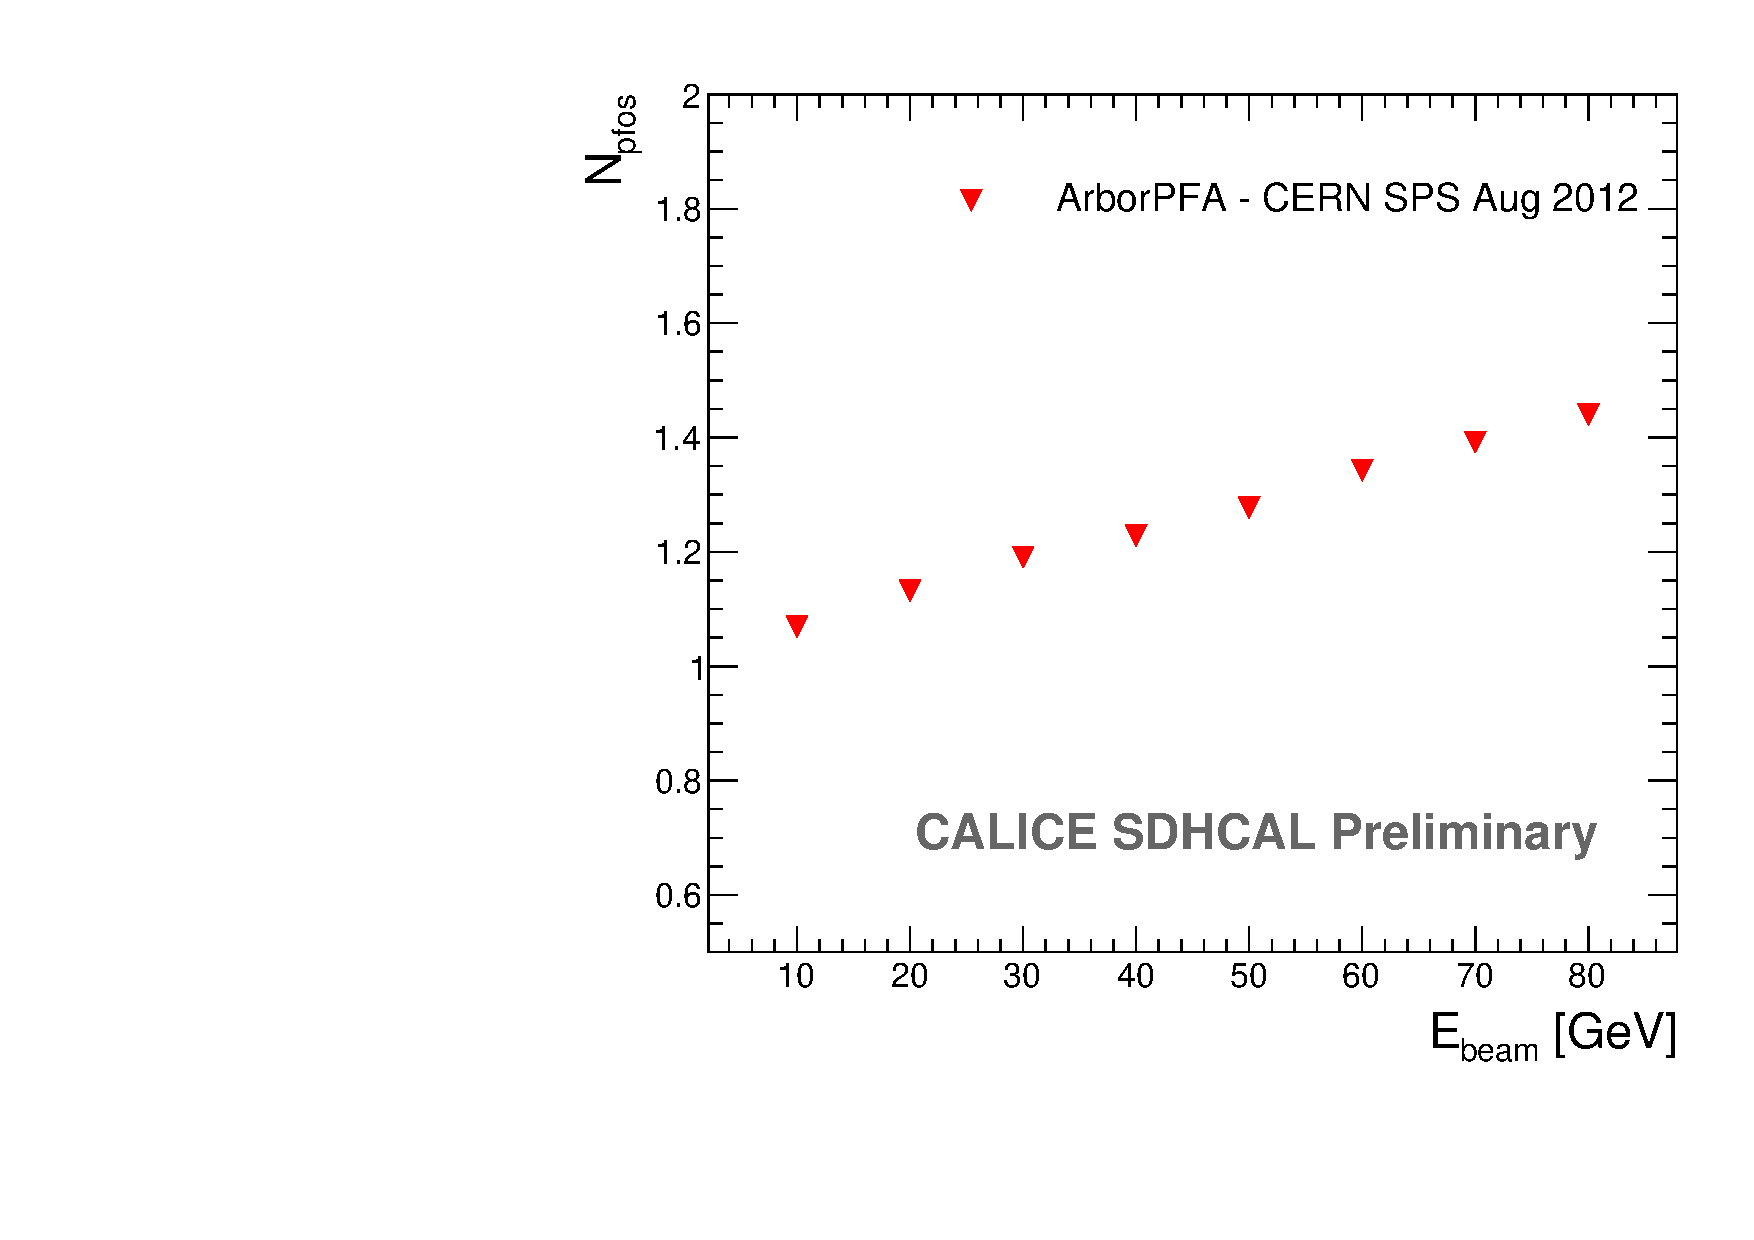
\includegraphics[width=0.45\linewidth]{SingleParticle_NPfos.pdf}
  \end{frame}
  
  %% Performance ArborPFA - single particle - plots
  \begin{frame}
  \frametitle{\secname}
  \framesubtitle{\subsecname}
    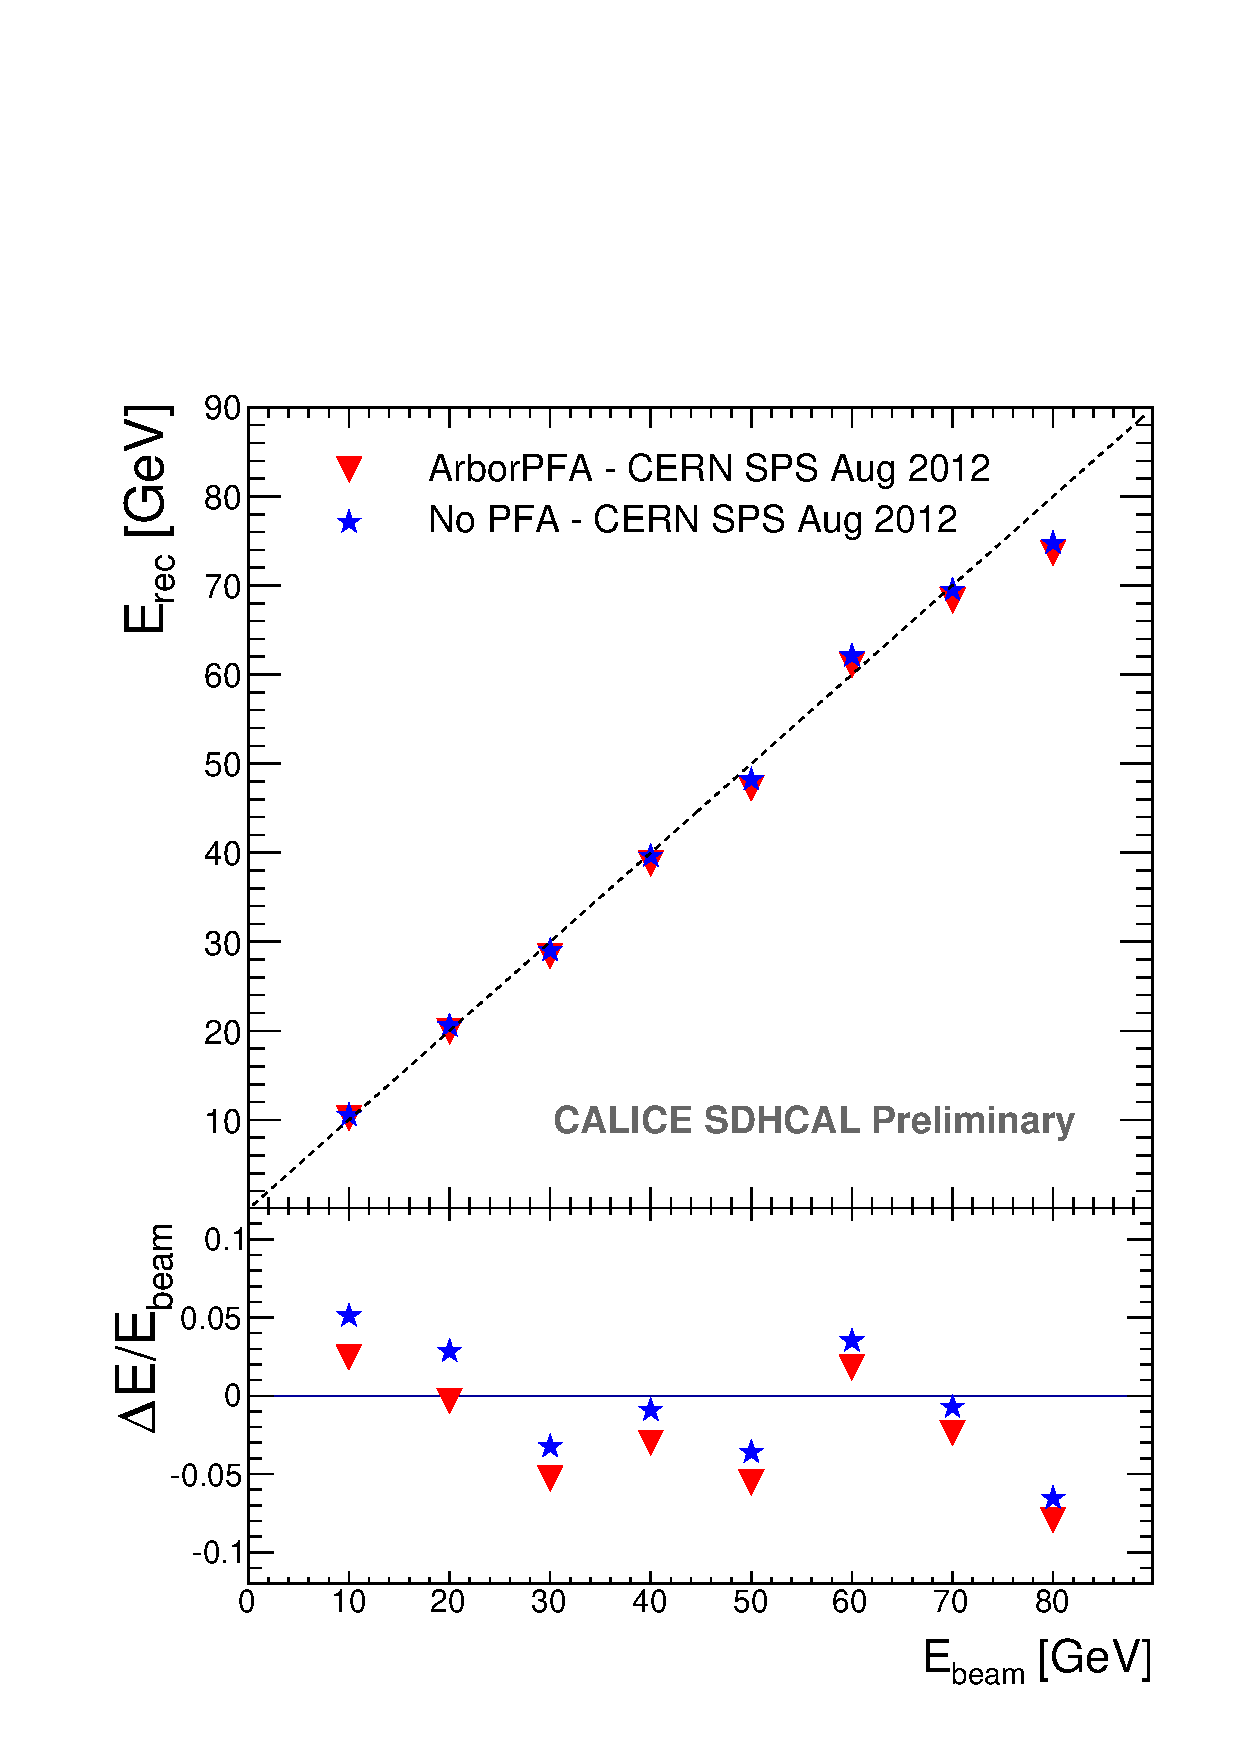
\includegraphics[width=0.45\linewidth]{SingleParticle_ERec.pdf}~
    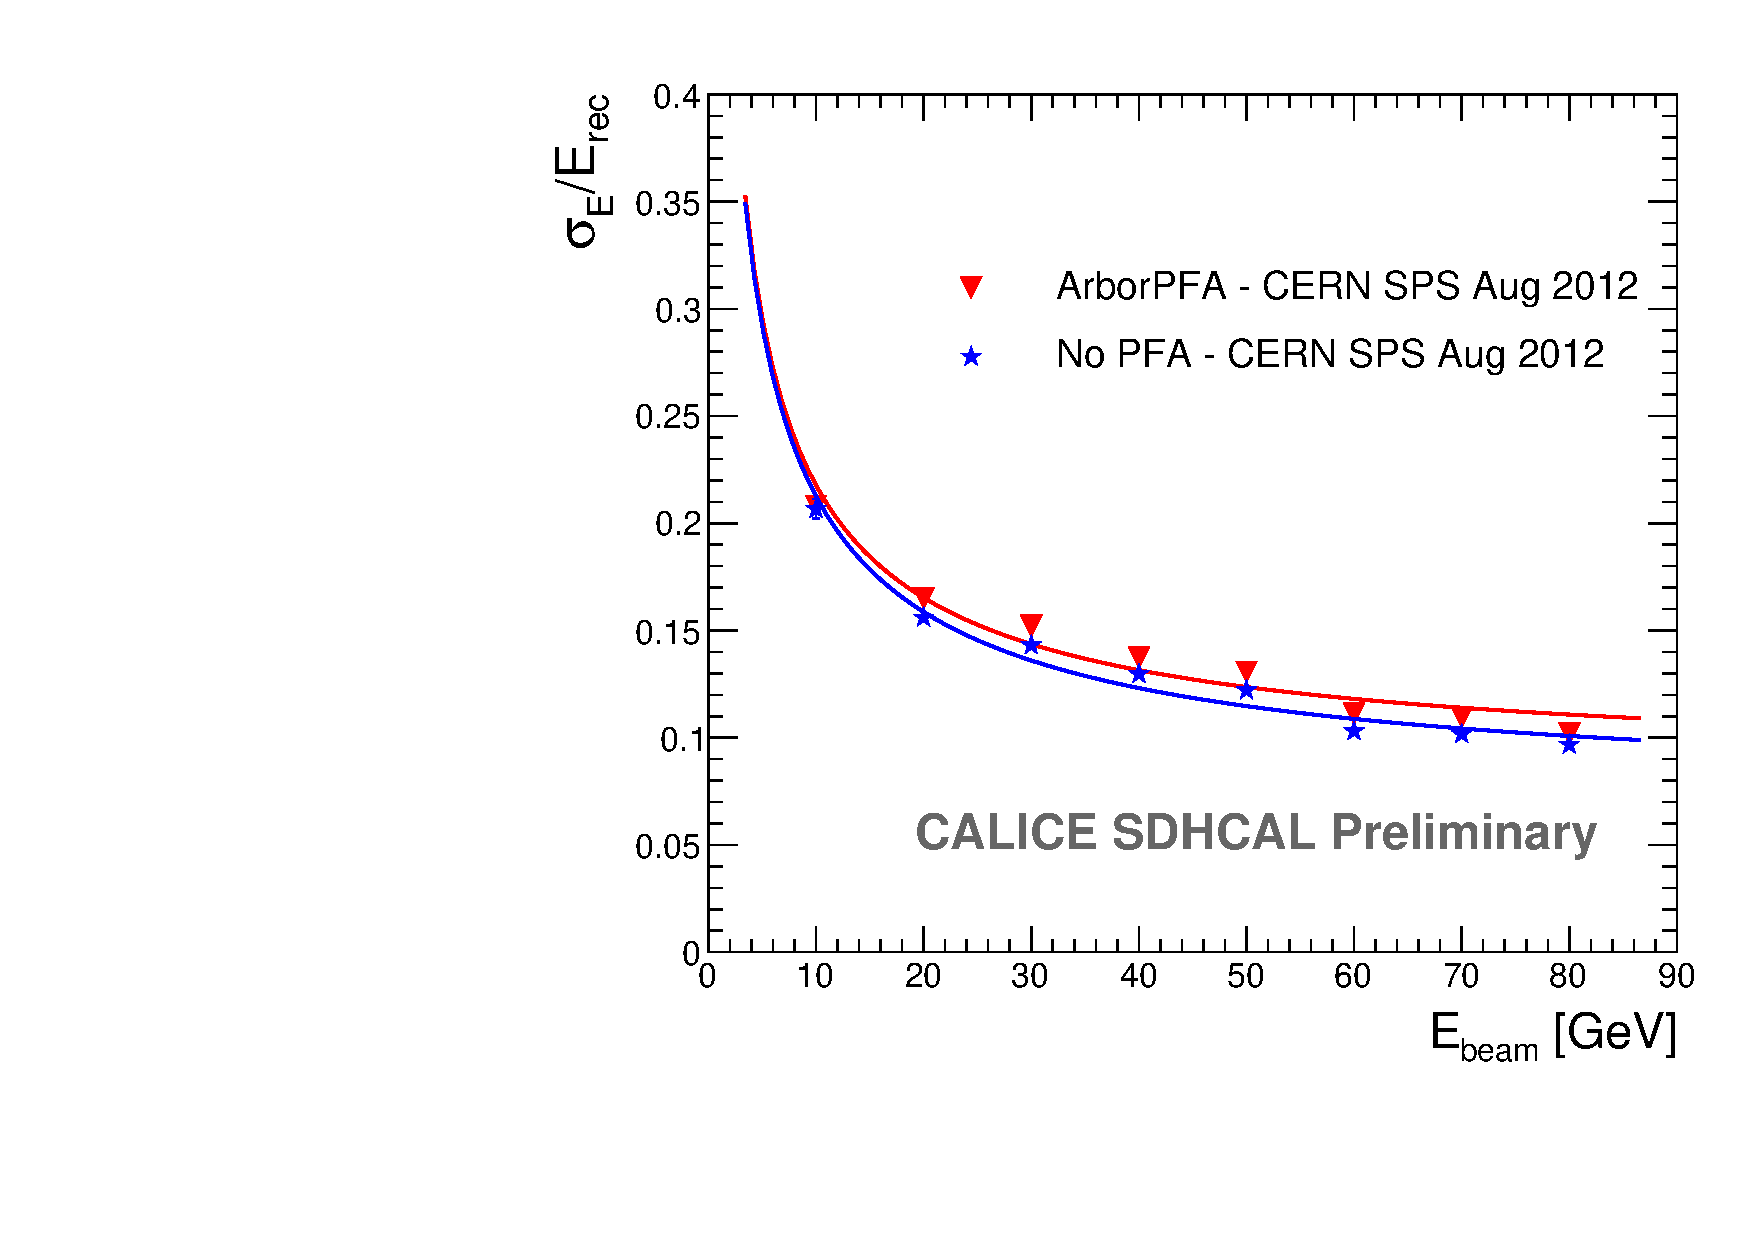
\includegraphics[width=0.45\linewidth]{SingleParticle_EResol.pdf}
  \end{frame}
  
  
  \subsection{Performance - Deux hadrons superposés}
  \begin{frame}
  \frametitle{\secname}
  \framesubtitle{\subsecname}
    \begin{block}{Superposition de deux événements hadronique}
      \begin{itemize}
        \item Même jeu de données
        \item Énergie particule 1 : 10 GeV
        \item Énergies particule 2 : [10 ; 50] GeV par pas de 10 GeV
      \end{itemize}
      Algorithme de superposition :
      \begin{itemize}
        \item Détermination des points d'entrées et barycentres.
        \item Suppression des hits du segment de trace primaire du hadron de 10 GeV
        \item Centrage au centre du calorimètre (x et y) puis décalage de $\pm$ d/2 dans la direction x
        \item Hit superposé : le seuil le plus haut est assigné à ce hit 
        \item Les hits sont étiqueté 1, 2 ou 3 (superposé).
      \end{itemize}
    \end{block}
    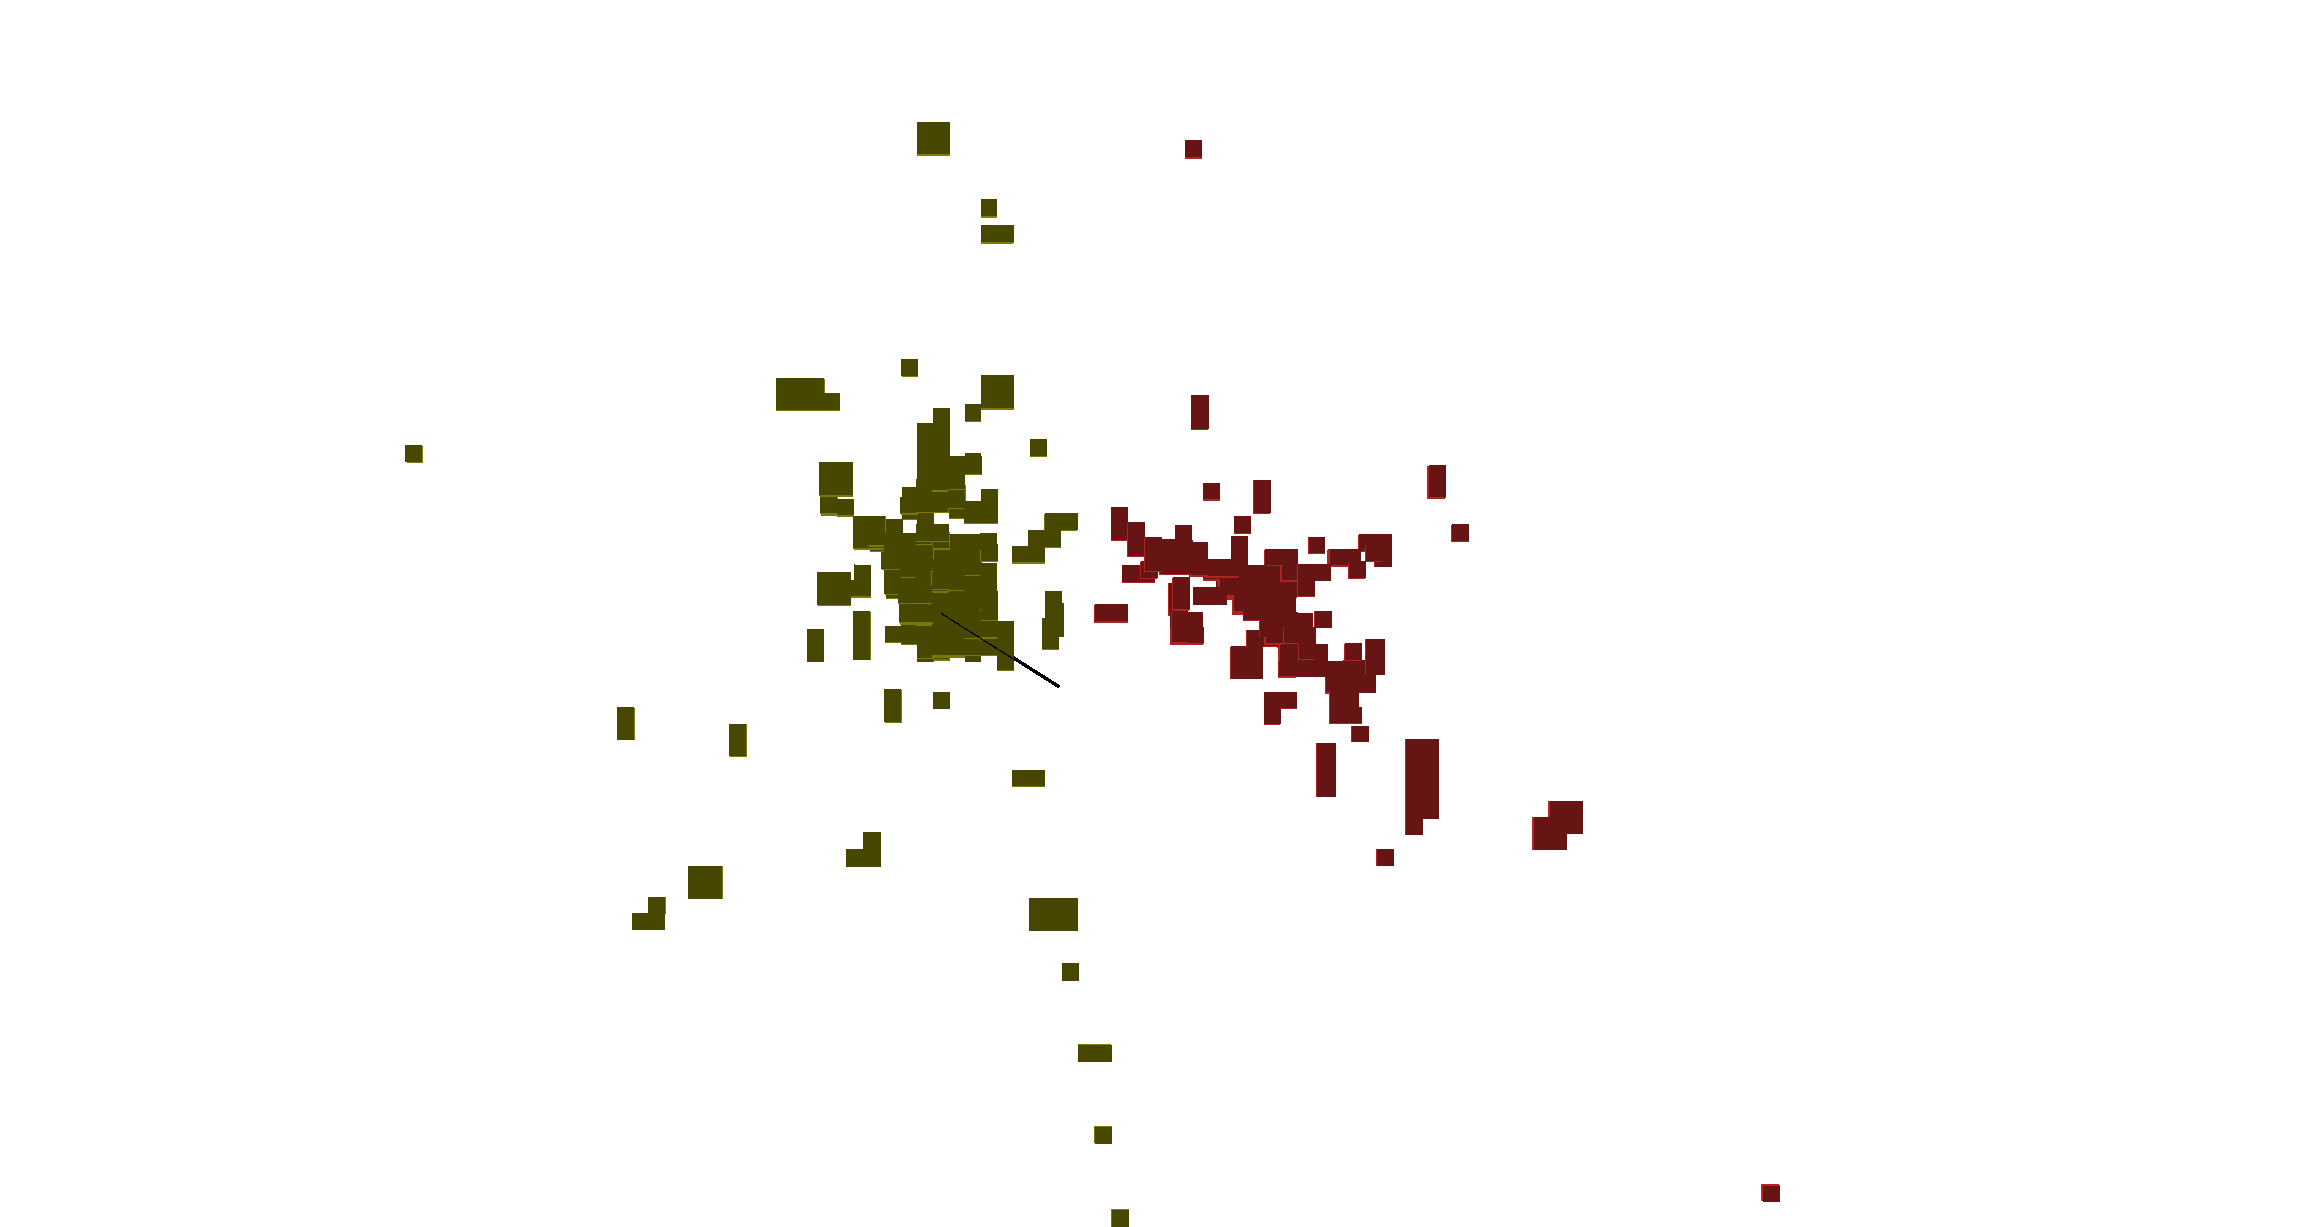
\includegraphics[width=0.32\linewidth]{ArborPFA_PandoraMonitoring_SDHCAL_Overlay_XY.pdf}
    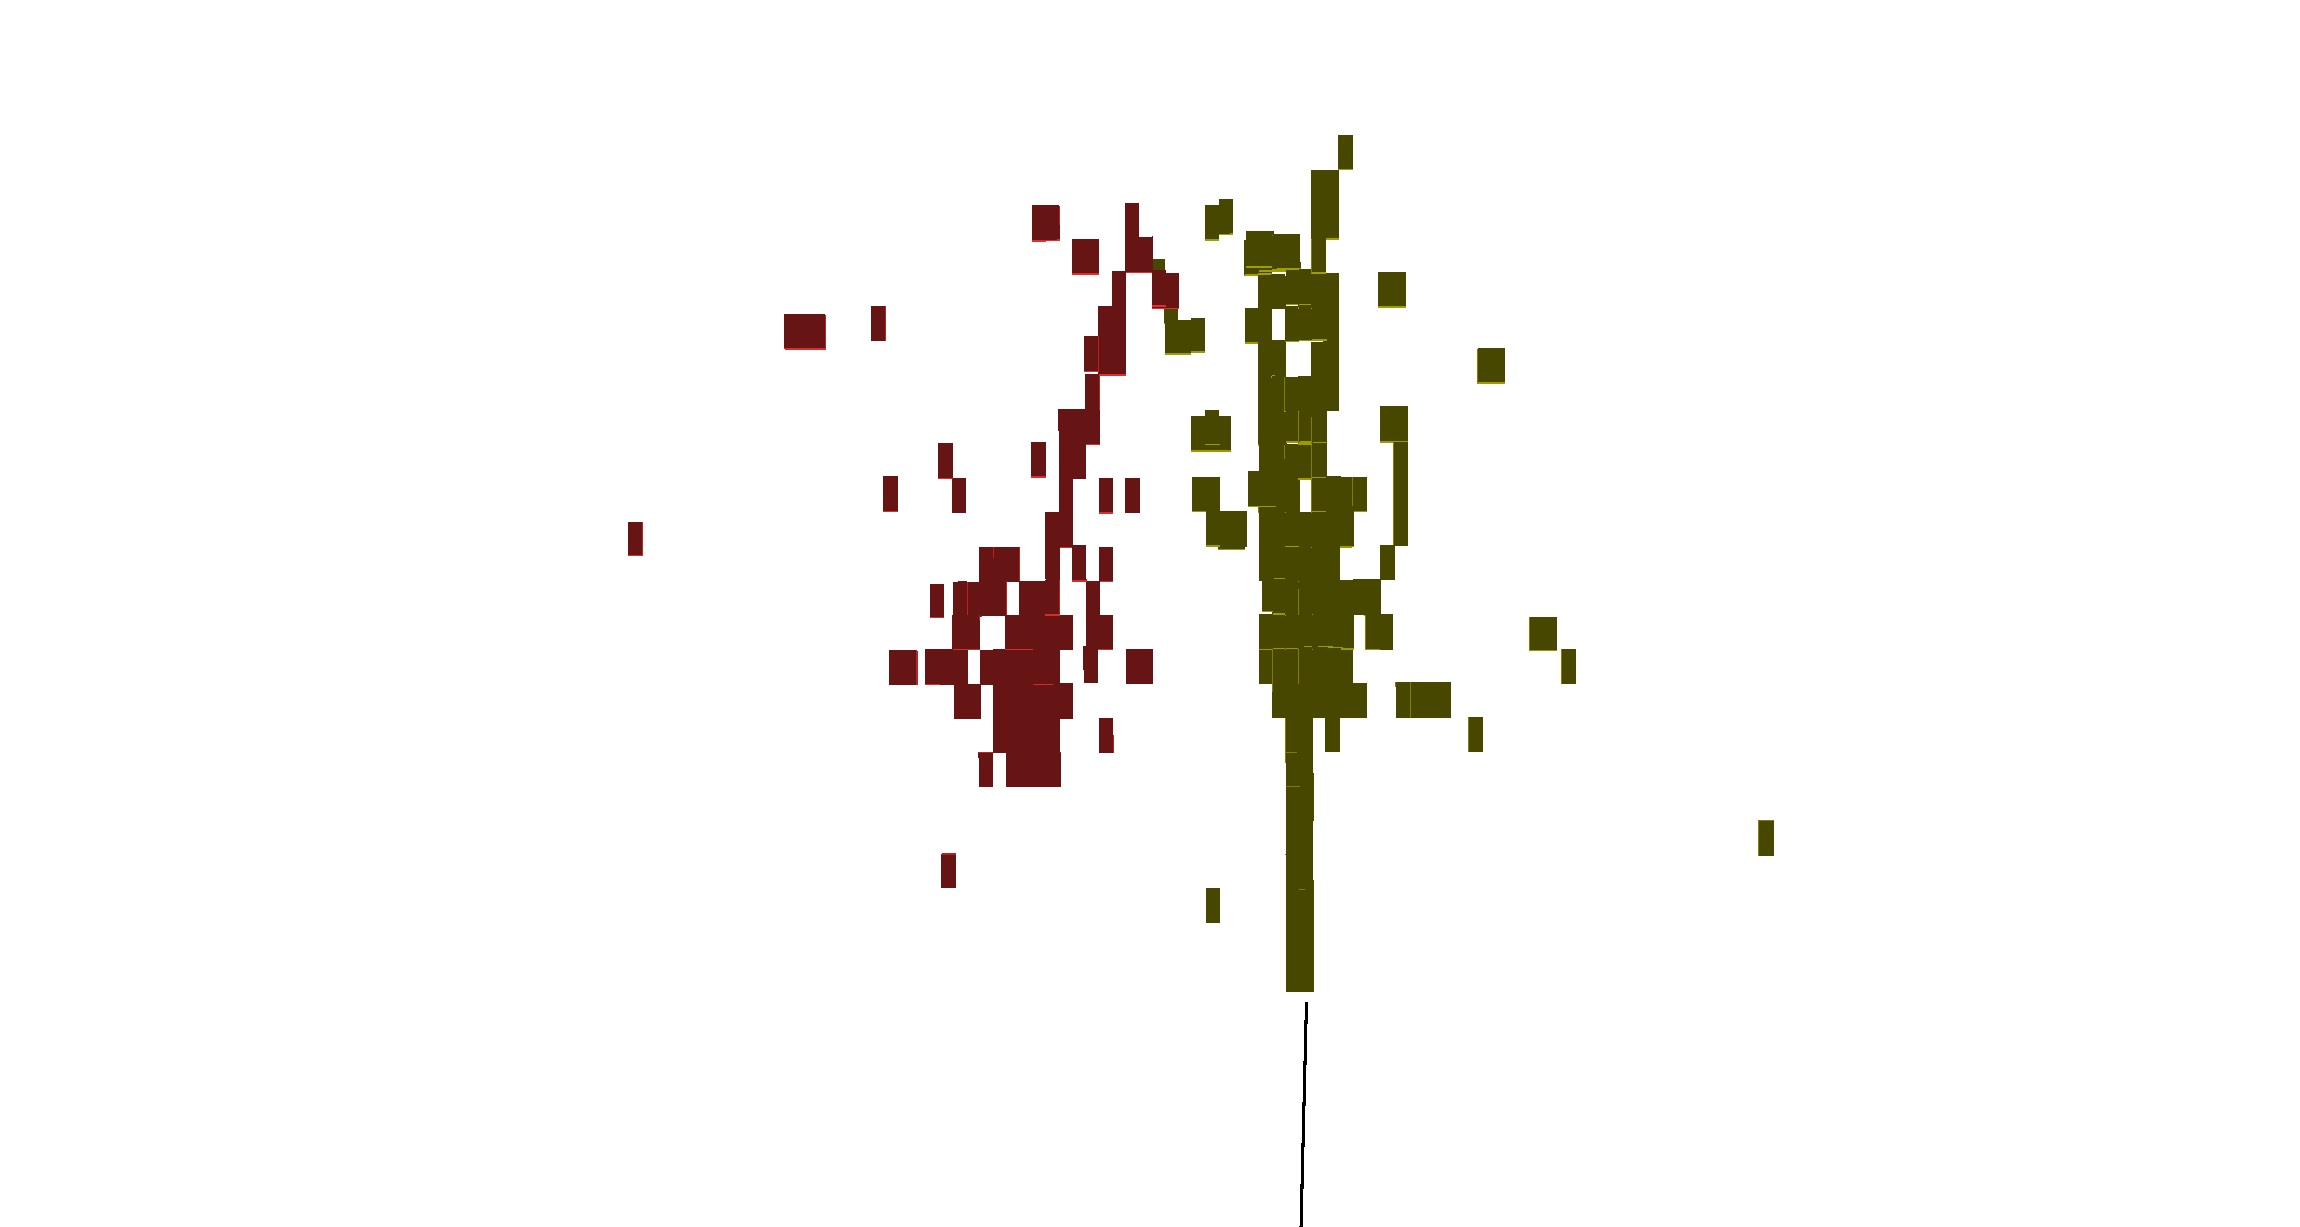
\includegraphics[width=0.32\linewidth]{ArborPFA_PandoraMonitoring_SDHCAL_Overlay_XZ.pdf}
    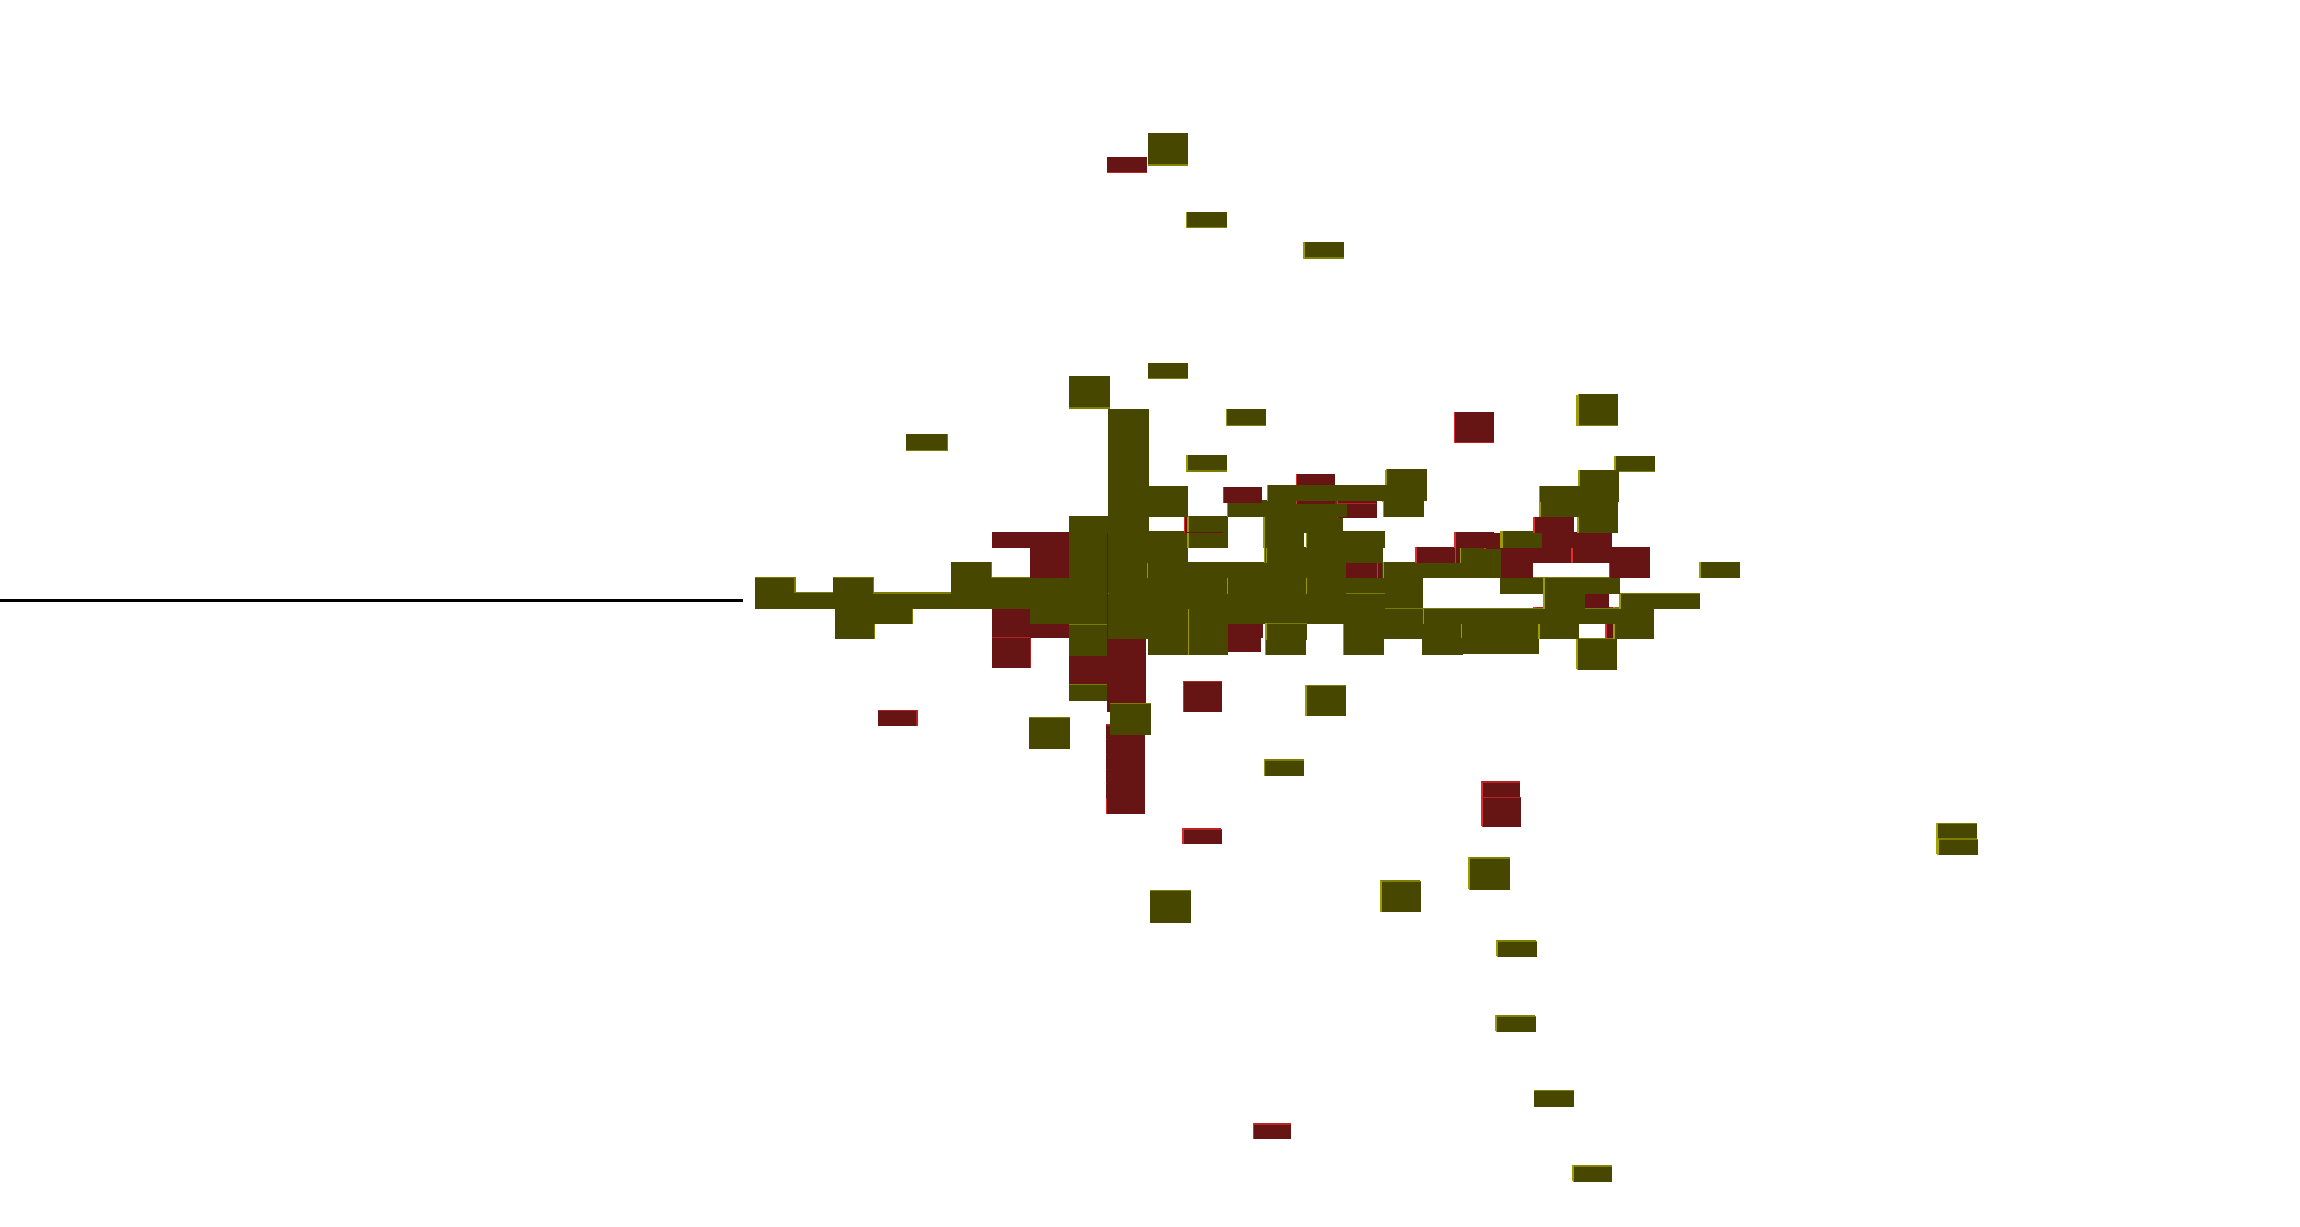
\includegraphics[width=0.32\linewidth]{ArborPFA_PandoraMonitoring_SDHCAL_Overlay_YZ.pdf}
  \end{frame}
  
 
  %% Overlay event - plots 2
  \begin{frame}
  \frametitle{\secname}
  \framesubtitle{\subsecname}
    
    \begin{minipage}{0.49\linewidth}
      \begin{center}
        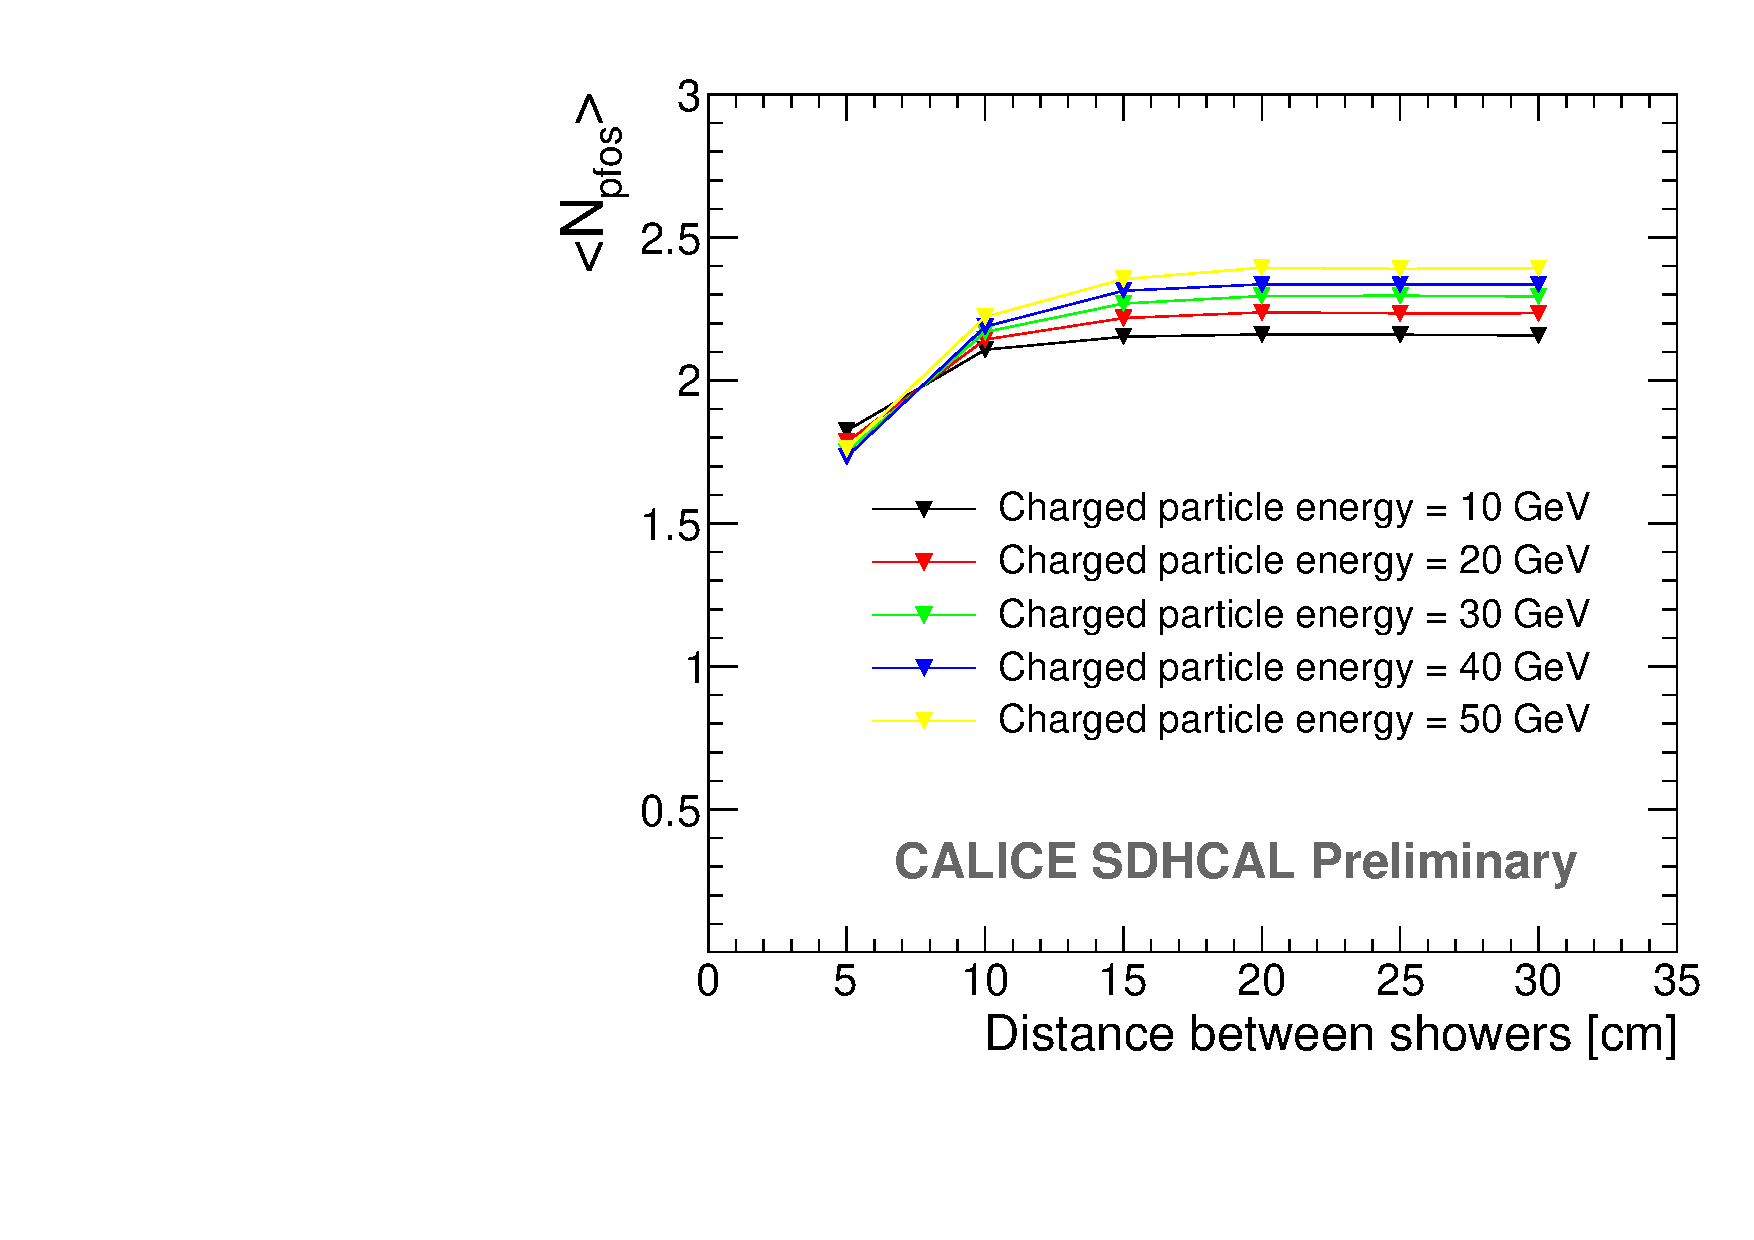
\includegraphics[width=0.8\linewidth]{OverlayEvent_NPfos.pdf}     
      \end{center}
    \end{minipage} \hfill
    \begin{minipage}{0.49\linewidth}
      \begin{block}{Efficacité et pureté}
        \begin{equation}
          \epsilon = \frac{Nhit_{good}}{Nhit_{ini,tot}}
        \end{equation}
        \begin{equation}
          \rho = \frac{Nhit_{good}}{Nhit_{rec,tot}}
        \end{equation}
      \end{block}
    \end{minipage}
    \begin{center}
      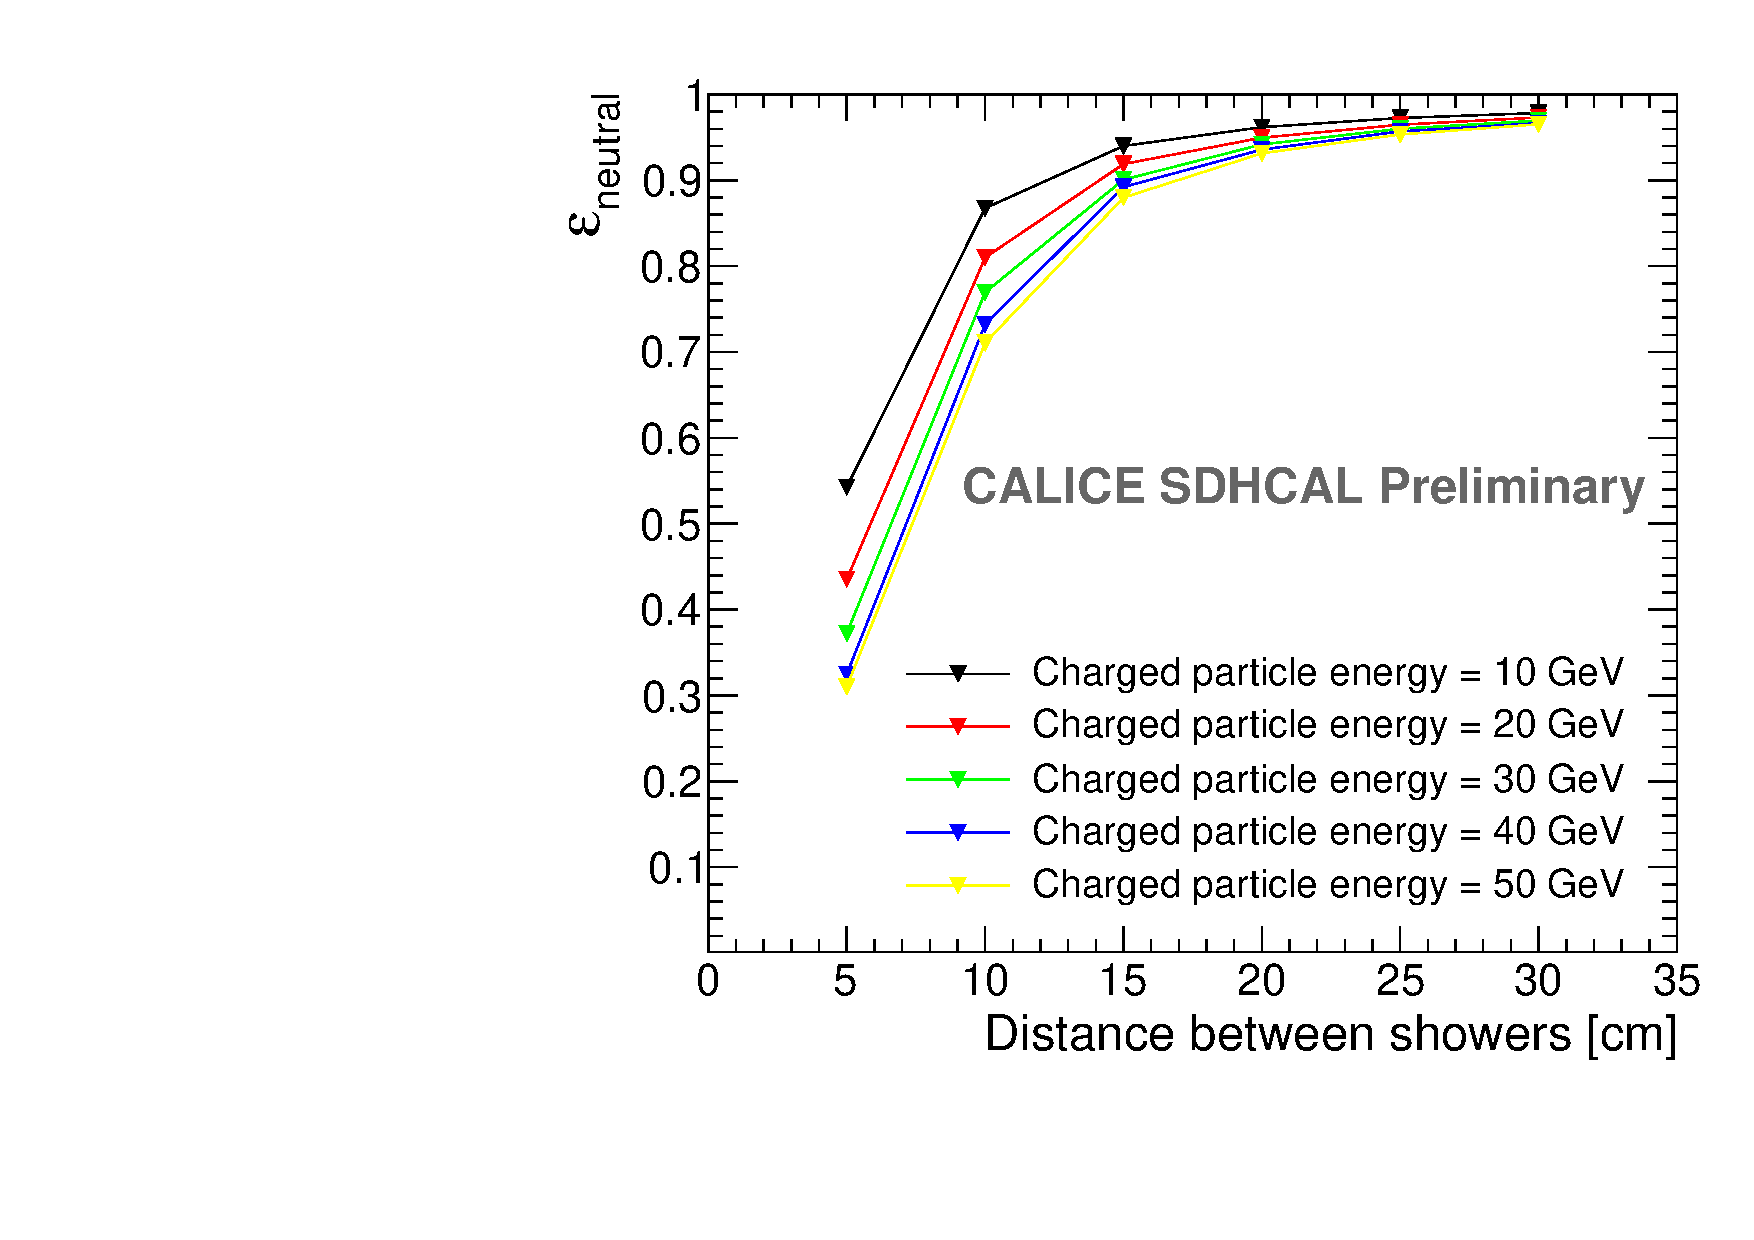
\includegraphics[width=0.4\linewidth]{OverlayEvent_NeutralEfficiency.pdf} ~~~~~~~~~~~~~~~~
      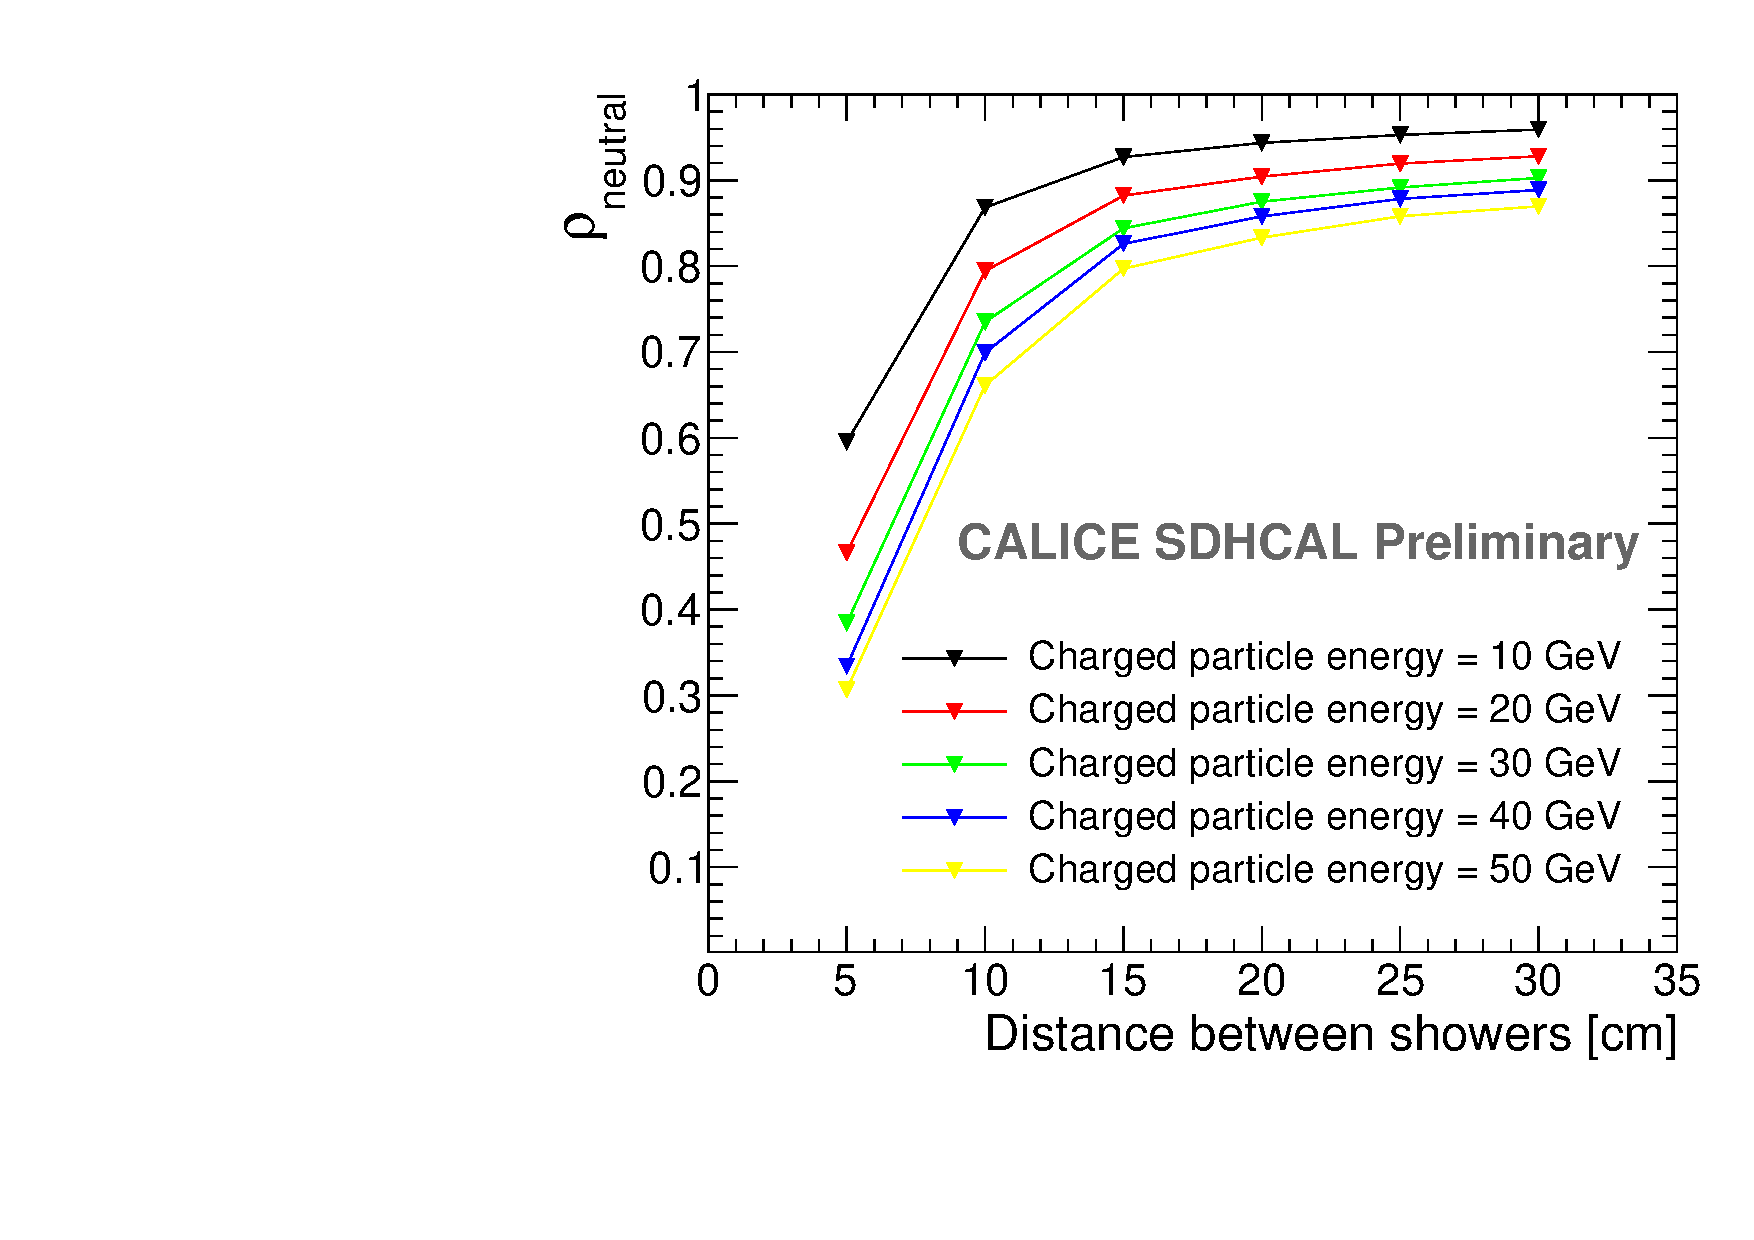
\includegraphics[width=0.4\linewidth]{OverlayEvent_NeutralPurity.pdf}     
    \end{center}
  \end{frame}


  %% Overlay event - plots 3
  \begin{frame}
  \frametitle{\secname}
  \framesubtitle{\subsecname}
    \begin{center}
      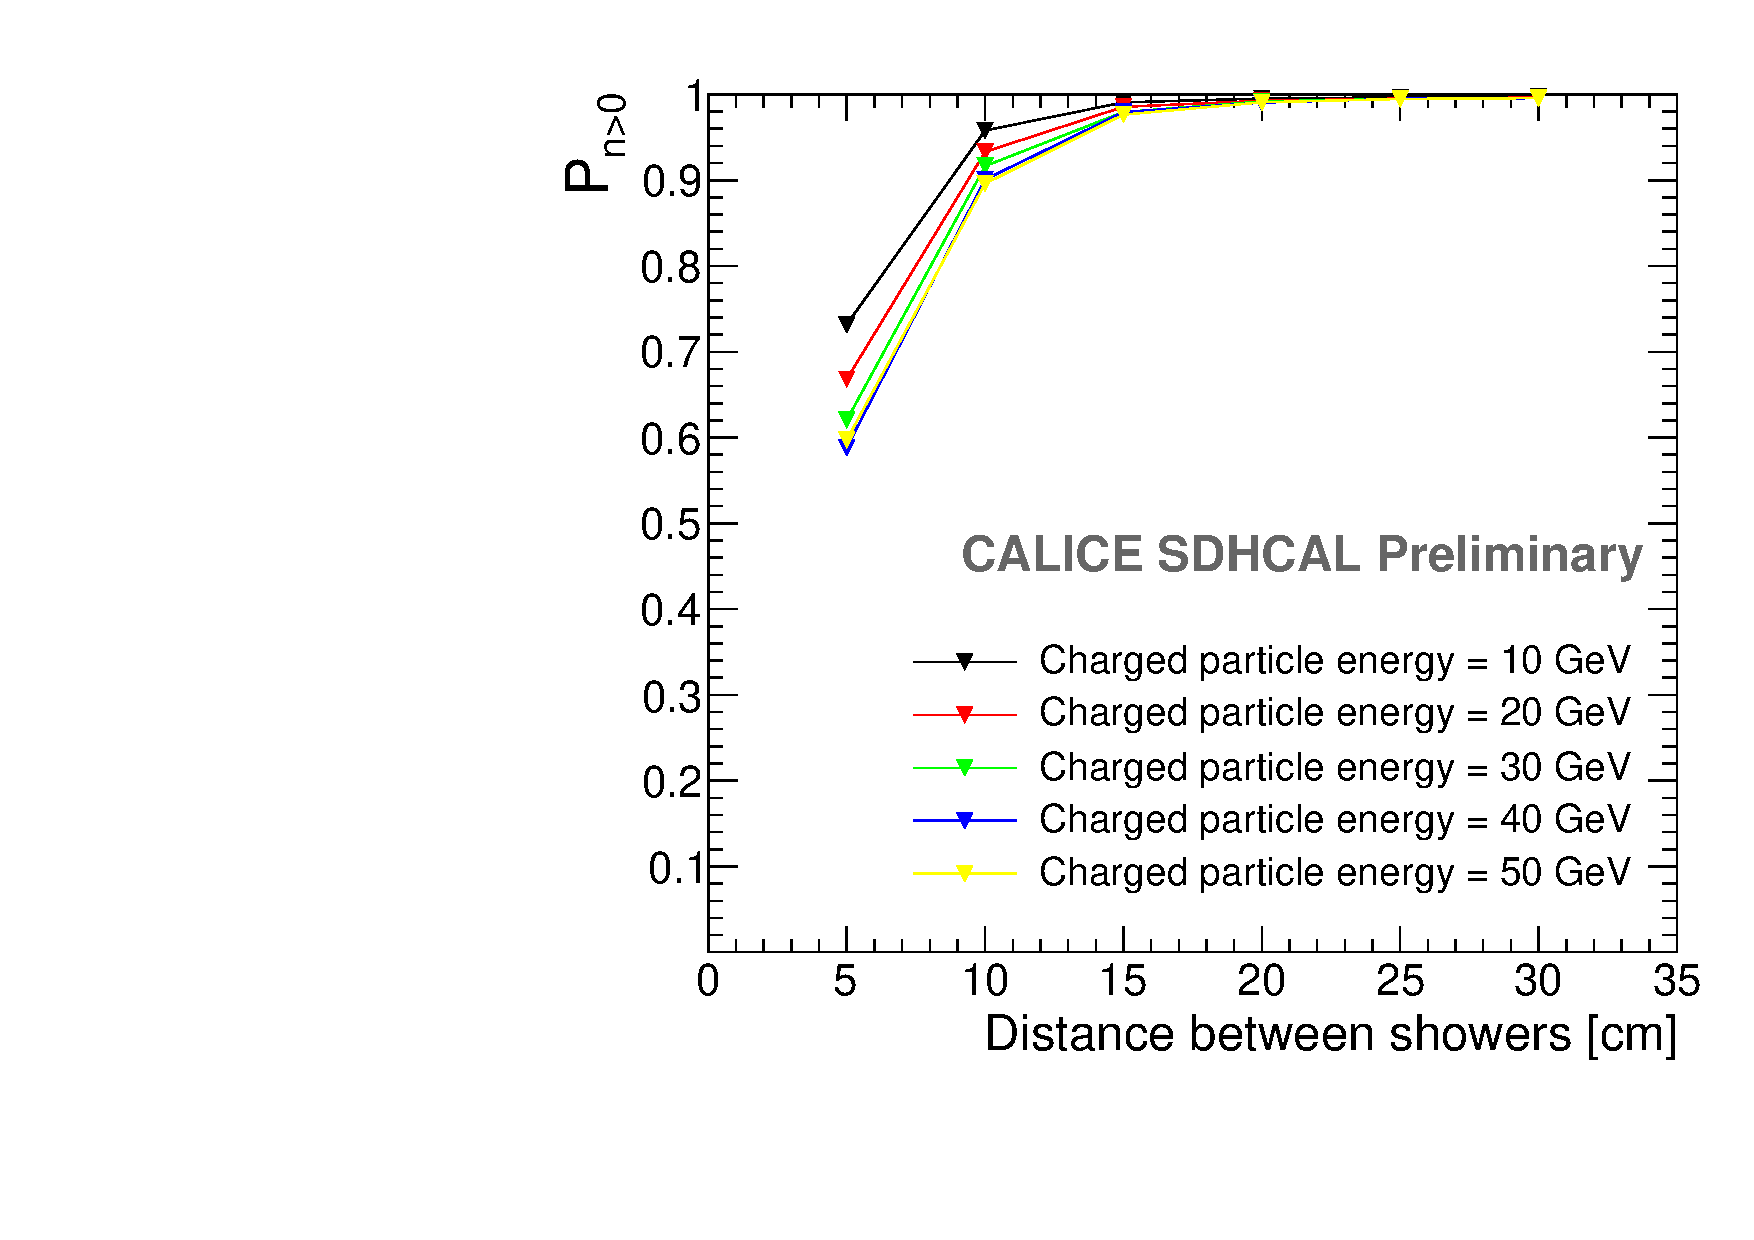
\includegraphics[width=0.48\linewidth]{OverlayEvent_NeutralPercentage.pdf}
      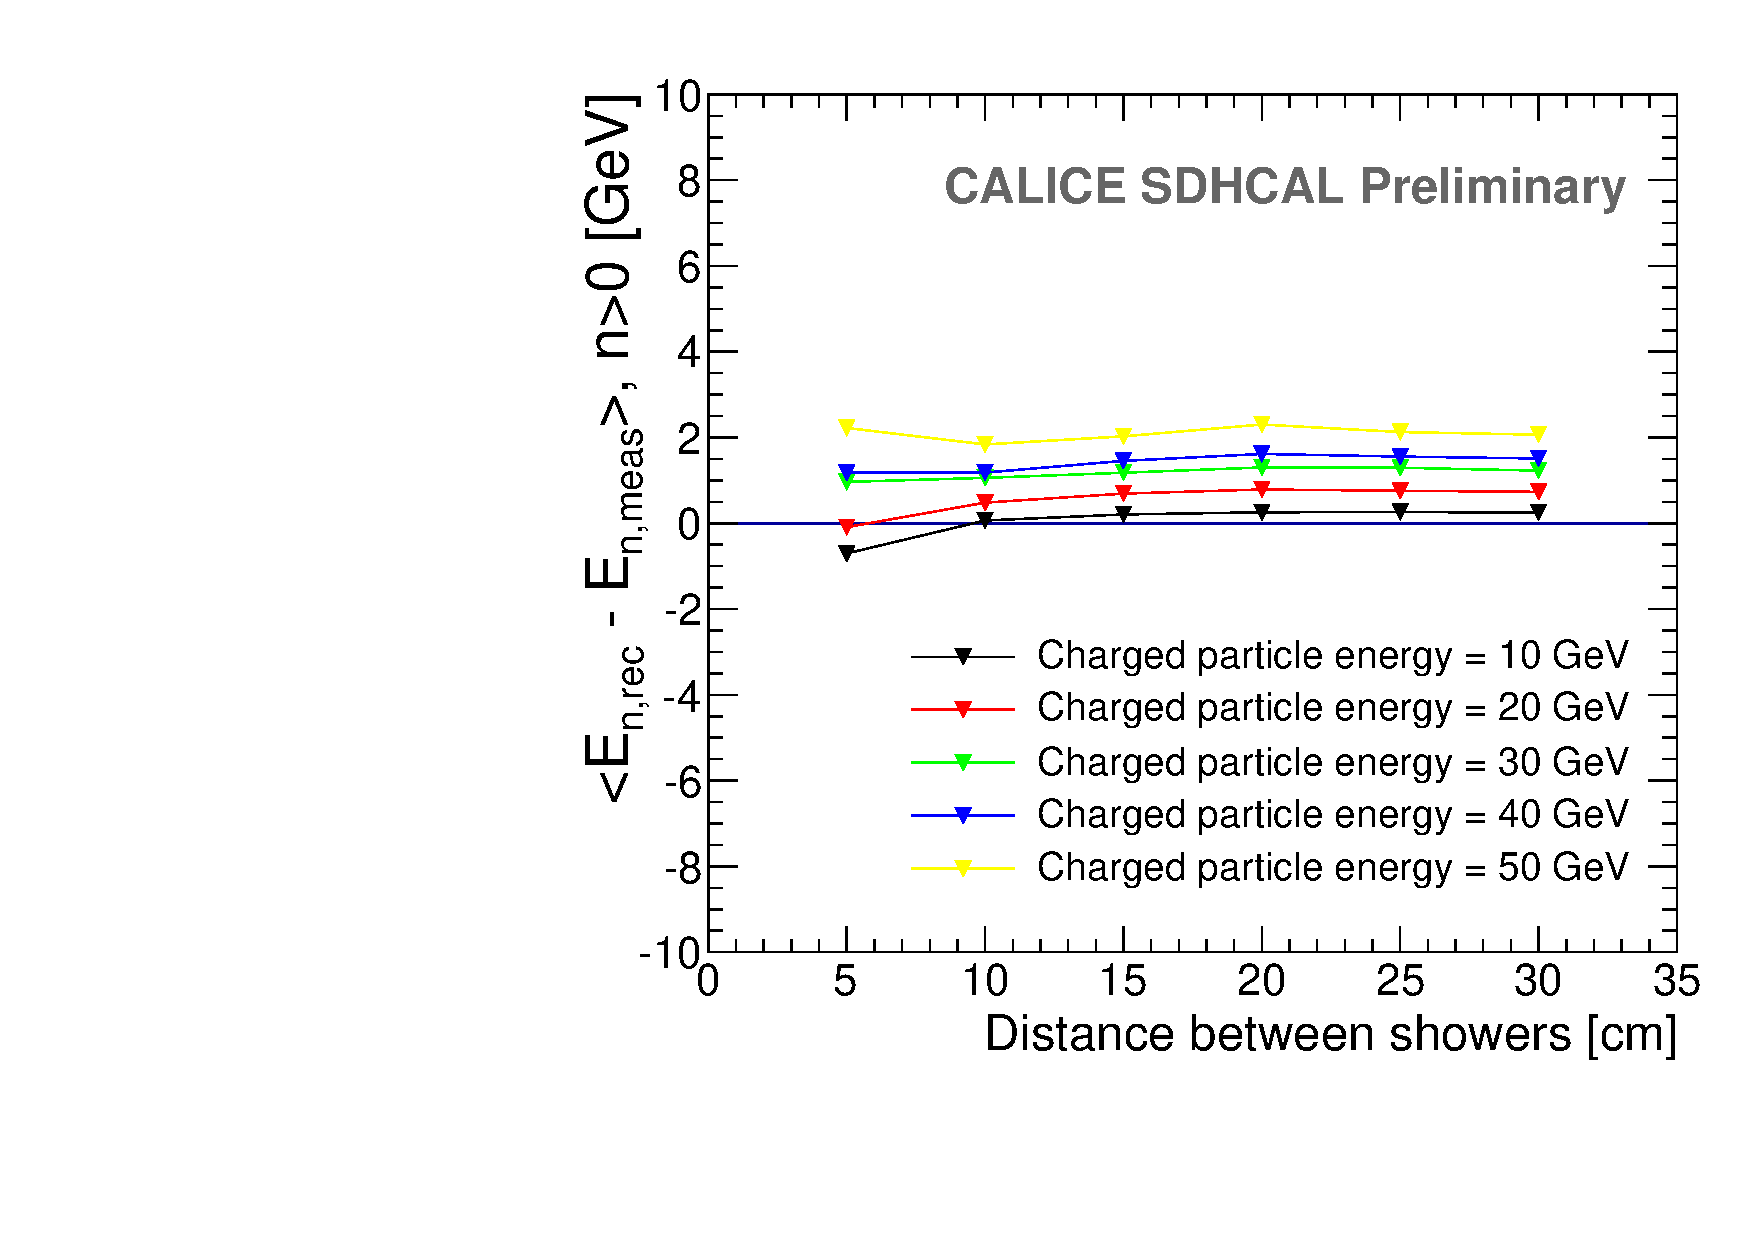
\includegraphics[width=0.48\linewidth]{OverlayEvent_NeutralEnergyDifferenceMeanNeutralEfficient.pdf}
    \end{center}
  \end{frame}
    
%%%%%%%%%%%%%%%%%
%% SYSTEME DQM %%
%%%%%%%%%%%%%%%%%
  \section{Monitoring de qualité de données}

  \begin{frame}
  \frametitle{\secname}
    \tableofcontents[currentsection]
  \end{frame}

  %% Introduction
  \subsection{Introduction}
  \begin{frame}
  \frametitle{\secname}
  \framesubtitle{\subsecname}
  \small
    \begin{block}{Les systèmes de DQM}
      \begin{itemize}
        \item Évalue la \textbf{qualité} des données :
        \begin{itemize}
          \item en ligne
          \item hors ligne
        \end{itemize}
        \item \textbf{Alerte} l'utilisateur d'un \textbf{état anormal du système} de détection (fuite de gaz, cellule morte, ...)
        \item Présents dans la plupart des expériences de physique de hautes énergies. Par exemple :
        \begin{itemize}
          \item CMS   - CMSSW DQM
          \item ALICE - AMORE
        \end{itemize}
      \end{itemize}
    \end{block}
    \pause
    \begin{minipage}{0.47\linewidth}
      \begin{block}{Fonctionnalités communes}
        \begin{itemize}
          \item Run control
          \item Analyse de données en ligne/hors ligne
          \item Tests de qualité des données
          \item Interface de visualisation des données (histogrammes, scalaires, etc ...)
          \item Environnements distribués
          \item Mise en relation à travers le réseau
          \item \textit{Workflow} du système
        \end{itemize}
      \end{block}
    \end{minipage} \hfill
    \begin{minipage}{0.47\linewidth}
      \begin{block}{Fonctionnalités différentes}
        \begin{itemize}
          \item Contenu des analyses
          \item Système d'acquisition
          \item \textbf{Format de données}
          \item Synthèse différente des données sur l'interface utilisateur
        \end{itemize}
      \end{block}
    \end{minipage}
  \end{frame}  
  
  
  %% DQM4HEP
  \subsection{DQM4HEP}
  
  \begin{frame}
  \frametitle{\secname}
  \framesubtitle{\subsecname - Data Quality Monitoring for High Energy Physics}
    \begin{block}{Points clés}
      \begin{itemize}
        \pause
        \item Run control standalone dédié au DQM
        \pause
        \item Système de plug-in par librairies partagées
        \pause
        \item \textbf{Distribution par réseau} des données brutes : collecteur (serveur), client
        \pause
        \item Analyse de données adaptée au DQM : type d'analyse, cycle
        \pause
        \item \textbf{Distribution par réseau} des histogrammes : collecteur (serveur), client
        \pause
        \item Interface de \textbf{visualisation des histogrammes} (Qt Gui)
        \pause
        \item Interface graphique de \textbf{gestion de processus} par réseau (Qt Gui)
        \pause
        \item \textbf{Modèle de données indépendant du format}
        \pause
        \item Interface ELog
      \end{itemize}
    \end{block}
    \pause
    \begin{block}{Dépendance}
      \begin{itemize}
        \item ROOT
        \item DIM (+ DIMJC)
        \item Json cpp (config)
        \item Optionnellement : LCIO, Qt, binaire Elog
      \end{itemize}
    \end{block}
    \textbf{Tout en C++ !!} \\
  \end{frame}
  
  %% Implementation réseau
  \begin{frame}
  \frametitle{\secname}
  \framesubtitle{\subsecname - Architecture réseau}
    \begin{center}
      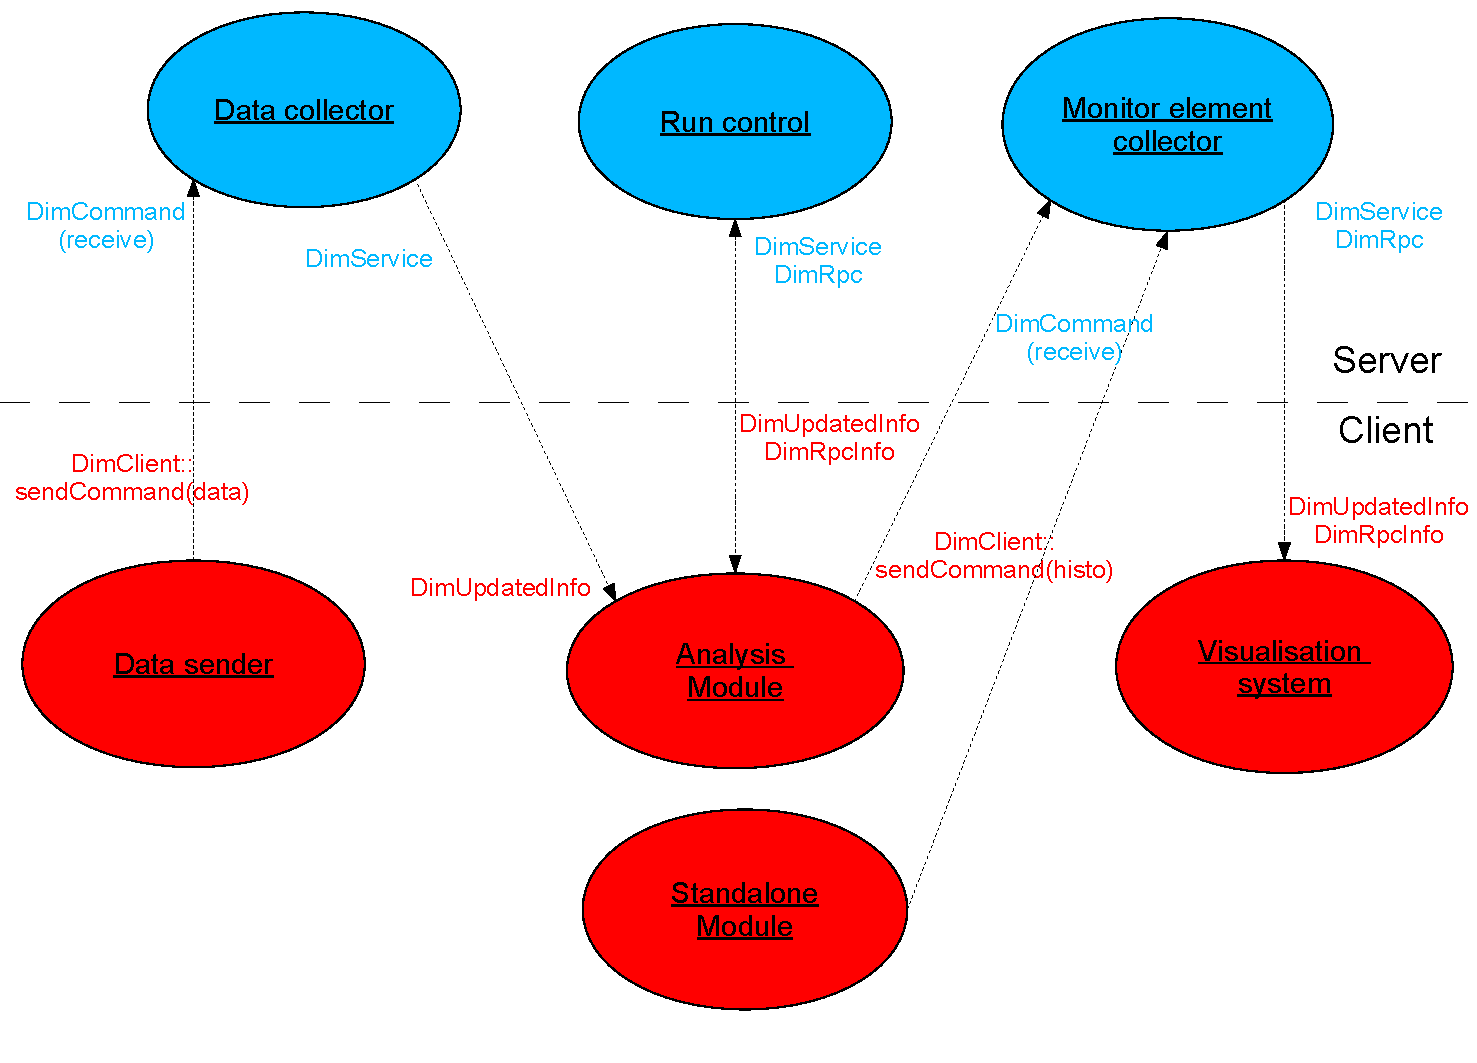
\includegraphics[width=\textwidth]{NetworkImplementation.pdf}        
    \end{center}    
  \end{frame}
  
  
%  \subsection{Interfaces}
  \begin{frame}
  \frametitle{\secname}
  \framesubtitle{\subsecname - Interface d'analyse de données}    
    \begin{minipage}{0.79\textwidth}
      \begin{block}{Module d'analyse}
        \begin{itemize}
          \item Conçu pour l'analyse de données (raw data, tracking, PFA)
          \item Produit des élements monitorables (histograms, scalaires, \textit{strings}, TObject)
          \item Structuré en séquence de runs et cycles
        \end{itemize}
      \end{block}
      \begin{itemize}
        \item \textbf{Init} : Initialisation de l'application, chargement des plugins, déclaration des services réseaux, etc...\\
        Attends un début de run
        \item \textbf{Start of run} : Commence une boucle de cycles
        \item \textbf{Start of cycle} : Commence une boucle de traitement de données
        \item \textbf{Process event} : Traite l’événement physique entrant, rempli les éléments monitorables, etc ...
        \item \textbf{End of cycle} : Termine un cycle. Récupère les éléments monitorables et les envoi au collecteur dédié
        \item \textbf{End of run} : Termine le run en cours. Attends le run suivant
        \item \textbf{End} : Quitte l'application
      \end{itemize}
    \end{minipage} \hfill
    \begin{minipage}{0.18\textwidth}
      \begin{flushright}
        \begin{tikzpicture}[scale=0.8]
        \node[draw] (I) at (0,-1) {Init};
        \node[draw] (SR) at (0,-2) {Start of run};
        \node[draw] (SC) at (0,-3) {Start of cycle};
        \node[draw] (PE) at (0,-4) {Process event};
        \node[draw] (EC) at (0,-5) {End of cycle};
        \node[draw] (ER) at (0,-6) {End of run};
        \node[draw] (E) at (0,-7) {End};
        \tikzset{fleche/.style={->,>=latex,thick}}
        \draw[fleche] (0,0) node {$\bullet$} -- (I);
        \draw[fleche] (I) -- (SR);
        \draw[fleche] (SR) -- (SC);
        \draw[fleche] (SC) -- (PE);
        \draw[fleche] (PE) -- (EC);
        \draw[fleche] (EC) -- (ER);
        \draw[fleche] (ER) -- (E);
        \draw[fleche] (E) -- (0,-8) node {$\bullet$};
        \draw[fleche] (0,-4.5) -- (1.3,-4.5) -- (1.3,-3.5) -- (0,-3.5);
        \draw[fleche] (0,-5.5) -- (1.4,-5.5) -- (1.4,-2.5) -- (0,-2.5);
        \draw[fleche] (0,-6.5) -- (1.5,-6.5) -- (1.5,-1.5) -- (0,-1.5);
        \end{tikzpicture}  
      \end{flushright}
    \end{minipage}
  \end{frame}
  

  \begin{frame}
  \frametitle{\secname}
  \framesubtitle{\subsecname - Interface d'analyse standalone}    
    \begin{minipage}{0.78\textwidth}
      \begin{block}{Module standalone}
        \begin{itemize}
          \item Conçu pour le traitement de données environementales (T, P, HV, LV, gaz)
          \item Pas de donnée transmise au module
          \item Produit des éléments monitorables (histograms, scalaires, \textit{strings}, TObject)
          \item Pas de structure en run
        \end{itemize}
      \end{block}
      \begin{itemize}
        \item \textbf{Init} : Initialise l'application, charge les plugins, etc ...
        \item \textbf{Start of cycle} : Démarre un cycle de n secondes
        \item \textbf{Process} : Fonction de rappel utilisateur
        \item \textbf{End of cycle} : Récupère les éléments monitorables et les envoi au collecteur dédié
        \item \textbf{End} : Quitte l'application
      \end{itemize}
    \end{minipage} \hfill
    \begin{minipage}{0.18\textwidth}
      \begin{flushright}
        \begin{tikzpicture}[scale=0.8]
        \node[draw] (I) at (0,-1) {Init};
        \node[draw] (SC) at (0,-2) {Start of cycle};
        \node[draw] (PE) at (0,-3) {Process};
        \node[draw] (EC) at (0,-4) {End of cycle};
        \node[draw] (E) at (0,-5) {End};
        \tikzset{fleche/.style={->,>=latex,thick}}
        \draw[fleche] (0,0) node {$\bullet$} -- (I);
        \draw[fleche] (I) -- (SC);
        \draw[fleche] (SC) -- (PE);
        \draw[fleche] (PE) -- (EC);
        \draw[fleche] (EC) -- (E);
        \draw[fleche] (E) -- (0,-6) node {$\bullet$};
        \draw[fleche] (0,-3.5) -- (1.3,-3.5) -- (1.3,-2.5) -- (0,-2.5);
        \draw[fleche] (0,-4.5) -- (1.4,-4.5) -- (1.4,-1.5) -- (0,-1.5);
        \end{tikzpicture}
      \end{flushright}
    \end{minipage}
  \end{frame}


  %% 
  \begin{frame}
  \frametitle{\secname}
  \framesubtitle{\subsecname - Interface réseau}
    \begin{block}{Interface vers le collecteur d'événement}
      \begin{itemize}
        \item envoi d'événements vers le collecteur
        \item requête d'événements au collecteur (avec/sans timeout)
        \item requête d'une \textbf{partie} de l'événement
        \item système interne de queue pour le stockage des événements
        \item mode de mise à jour automatique
      \end{itemize}
    \end{block}
    \begin{block}{Interface vers le collecteur d'éléments monitorables}
      \begin{itemize}
        \item Requêtes possibles :
        \begin{itemize}
          \item Information sur le collecteur (nom, machine, statistique, etc ...)
          \item Liste des noms des éléments monitorables + filtre (nom du module, type d'élément, ...)
          \item Liste d'éléments monitorables
        \end{itemize}
      \end{itemize}
    \end{block}
  \end{frame}
  
  
%   \begin{frame}
%   \frametitle{\secname}
%   \framesubtitle{\subsecname - Interface programmable (API)}
%   \scriptsize
%     \begin{block}{DQMModuleApi}
%       Responsable des opérations par/sur les modules d'analyse et au éléments y touchant directement
%       \begin{itemize}
%         \item \textit{Booking} d'éléments monitorables
%         \item Stockage structuré en répertoire
%         \item Tests de qualité sur les éléments monitorables :
%         \begin{itemize}
%           \item Test de $\chi^2$
%           \item Ajustement de fonction utilisateur
%           \item Moyenne d'un histogramme dans un intervalle
%           \item Test de Kolmogorov
%           \item Autres tests définis par l'utilisateur 
%         \end{itemize}
%         \item Résultats des tests de qualité
%         \item Gestion d'allocation/suppression mémoire des objets utilisateur
%       \end{itemize}
%     \end{block}
%     \begin{block}{Interface streaming}
%     Responsable de la \textit{sérialisation} des données (événement, élément monitorable, ...)
%       \begin{itemize}
%         \item DQMDataStream :
%         \begin{itemize}
%           \item Gestion lecture/écriture
%           \item Gestion du buffer
%         \end{itemize}
%         \item Interface DQMStreamerPlugin : 
%         \begin{itemize}
%           \item sérialise/désérialise un objet C++
%           \item ajout automatique au framework
%         \end{itemize}
%         \item DQMEvent : Wrapper autour d'un événement physique utilisateur (EVENT::LCEvent, edm::Event)
%       \end{itemize}
%     \end{block}
%   \end{frame}
  
  \begin{frame}
  \frametitle{\secname}
  \framesubtitle{\subsecname - Interface graphique - Run control}

    \begin{minipage}{0.3\linewidth}
      \includegraphics[width=1.3\linewidth]{RunControl.png}
    \end{minipage} \hfill
    \begin{minipage}{0.6\linewidth}
      \begin{block}{Run control}
        \begin{itemize}
          \item Envoie les signaux de début et fin de run
          \item Configuration du run : numéro de run, nom du détecteur, description et paramètres
          \item Montre le statut du run (started/stopped) et ses informations relatives
          \item Barre de notification
        \end{itemize}
      \end{block}
    \end{minipage}
  \end{frame}
  

  \begin{frame}
  \frametitle{\secname}
  \framesubtitle{\subsecname - Interface graphique - Gestion des processus}
    \includegraphics[width=\linewidth]{JobInterface.png} \\
    \begin{itemize}
      \item Charge une liste d’exécutables et leurs paramètres (hôte, nom, fichier source, etc ...) et montre leur statuts sur le réseau
      \item Configuration avec des fichiers Json
      \item Gestion des processus (start, kill) sur tous les hôtes qui fonctionne avec le DQM
    \end{itemize}
  \end{frame}
  

  \begin{frame}
  \frametitle{\secname}
  \framesubtitle{\subsecname - Interface graphique - Fenêtre de monitoring}
  \begin{center}
    \begin{overlayarea}{\linewidth}{0.6\linewidth}
      \includegraphics[width=\linewidth]<1>{MonitoringControl.png}
      \includegraphics[width=\linewidth]<2>{MonitoringControl_DirectoryStructure.png}
      \includegraphics[width=\linewidth]<3>{MonitoringControl_CanvasArea.png}
      \includegraphics[width=\linewidth]<4>{MonitoringControl_UpdateMode.png}
      \includegraphics[width=\linewidth]<5>{MonitoringControl_OpenBrowser.png}
    \end{overlayarea}
  \end{center}
%     \footnotesize
%     \begin{itemize}
%       \item Interface de query (Browser) pour construire une sélection d'éléments monitorable à afficher
%       \item Structure en dossier sur la gauche
%       \item Plusieurs aires de tracage d'éléments disponible sur la droite
%       \item Les éléments tracés sont des objet ROOT (pas des images) $\rightarrow$ interactions ROOT habituelles disponibles (zoom, fit, etc ...)
%       \item Mode automatique "query and display" avec un chronomètre (n secondes) 
%       \item Résultats des tests de qualités accessibles depuis l'interface
%     \end{itemize}
  \end{frame}

  
  \begin{frame}
  \frametitle{\secname}
  \framesubtitle{\subsecname - Interface graphique - Fenêtre de navigation}
    \begin{overlayarea}{\linewidth}{0.6\linewidth}
      \begin{center}
        \includegraphics[width=0.6\linewidth]<1>{MonitoringBrowser.png}
        \includegraphics[width=0.6\linewidth]<2>{MonitoringBrowser_Collector.png}
        \includegraphics[width=0.6\linewidth]<3>{MonitoringBrowser_Search.png}
        \includegraphics[width=0.6\linewidth]<4>{MonitoringBrowser_SearchResult.png}
        \includegraphics[width=0.6\linewidth]<5>{MonitoringBrowser_ReplaceAppend.png}
      \end{center}
    \end{overlayarea}
  \end{frame}
  
  

  

  
  
  
  \subsection{Implémentation pour le SDHCAL}  

  \begin{frame}
  \frametitle{\secname}
  \framesubtitle{\subsecname - Implémentation pour le SDHCAL (actuelle)}
    \begin{center}
      \includegraphics[width=0.8\linewidth]{dqm_sdhcal_current_impl.pdf}    
    \end{center}
  \end{frame}
  
  
  \begin{frame}
  \frametitle{\secname}
  \framesubtitle{\subsecname - Implémentation pour le SDHCAL (prévue)}
    \begin{center}
      \includegraphics[width=0.85\linewidth]{dqm_sdhcal_future_impl.pdf}    
    \end{center}
  \end{frame}
      
  \section{Conclusion et perspectives}
  
  \begin{frame}
  \frametitle{\secname}
    \tableofcontents[currentsection]
  \end{frame}
  
  %% Conclusion
  \begin{frame}
  \frametitle{\secname}
  \framesubtitle{Conclusion}
    \begin{block}{Algorithme de suivi de particules}
      \begin{itemize}
        \item Développement d'un algorithme de suivi de particule basé sur la topologie en arbre pour le prototype SDHCAL
        \item Extraction des performances pour un hadron seul - OK
        \item Extraction des performances pour des hadron proches - OK jusqu'à 5 cm de séparation
      \end{itemize}
      Note interne CALICE soumise : \textbf{CAN-054 Editorial Board}
    \end{block}
    \begin{block}{Monitoring de qualité des données}
      \begin{itemize}
        \item Développement d'un outil de monitoring en ligne
        \item Jeu d'interfaces pour l’utilisateur :
        \begin{itemize}
          \item Analyse de données
          \item Sérialisation
          \item Interfaces réseaux
          \item Interfaces graphiques
        \end{itemize}
        \item Premiers déploiements pour le prototype SDHCAL
      \end{itemize}
    \end{block}
  \end{frame}

  %% Perspectives  
  \begin{frame}
  \frametitle{\secname}
  \framesubtitle{Perspectives}
    \begin{block}{Algorithme de suivi de particules}
      \begin{itemize}
        \item Correction de certains algorithmes $\rightarrow$ revoir les performances (à faire)
        \item Implémentation dans l'ILD :
        \begin{itemize}
          \item Correction angulaire pour les connexions (avancé)
          \item Utilisation du tracking plus élaboré (commencé)
          \item Implémentation dans le ECAL (commencé)
          \item Algorithme de reconstruction pour les muons (à faire)
          \item Reconstruction des photons déléguée à GARLIC (commencé)
          \item Calibration en énergie (à faire)
        \end{itemize}
        \item Performances physique :
        \begin{itemize}
          \item Résolution en énergie des jets (JER) (à faire)
          \item Échelle d'énergie des jets (JES) (à faire)
          \item Étude d'un canal physique (e+e- $\rightarrow$ HZ) (à faire)
        \end{itemize}
      \end{itemize}
    \end{block}
    \begin{block}{Monitoring de qualité des données}
      \begin{itemize}
        \item Revoir certaines parties de l'architecture :
        \begin{itemize}
          \item Pattern MVC pour l'interface graphique de monitoring (à faire)
          \item Codage du workflow dans les applications de modules (commencé)
        \end{itemize}
        \item Développement d'outils hors ligne (commencé)
        \item Implémentation des modules pour le SDHCAL (à faire)
        \item Implémentation pour un test en faisceau combiné avec un ECal (à faire)
      \end{itemize}
    \end{block}
  \end{frame}


  \begin{frame}
  ~ \\
  ~ \\
  ~ \\
  ~ \\
  ~ \\
  ~ \\
    \centering \large Merci pour votre attention !
  ~ \\
  ~ \\
  ~ \\    
  \end{frame}


  

  \section*{Backup}

  \begin{frame}
  \frametitle{\secname}
  \framesubtitle{Reconstruction et sélection des événements}
    \begin{minipage}{0.4\linewidth}
      \includegraphics[width=\linewidth]{sdhcal_time_spectrum.png}
    \end{minipage} \hfill
    \begin{minipage}{0.58\linewidth}
      \begin{block}{Reconstruction : \textit{clustering} en temps}
        \begin{itemize}
          \item Minimum NHit : 7
          \item Fenêtre en temps : $\pm$ 2
        \end{itemize}
      \end{block}
    \end{minipage}
    \pause
    \begin{minipage}{0.6\linewidth}
      \begin{block}{Sélection des événements hadroniques}
      Pas de détecteur cherenköv $\rightarrow$ sélection topologique
        \begin{itemize}
          \item Muon : NHit/N$_{layer}$ > 2.2
          \item Particules neutres : NHit $\in$ 5 premiers plans $\geq$ 4
          \item Muon radiatifs : $\frac{N_{touched~layers}/RMS>5cm}{N_{touched~layers}}$ < 20 \%
          \item Electrons : Z$_{begin}$ $\geq$ 5 et N$_{touched~layers}$ $\geq$ 30
        \end{itemize}
      \end{block}
    \end{minipage} \hfill
    \begin{minipage}{0.38\linewidth}
      \includegraphics[width=\linewidth]{sdhcal_hadron_selection_40GeV.pdf}
    \end{minipage}
  \end{frame}
  

  \begin{frame}
  \frametitle{\secname}
  \framesubtitle{ArborPFA - La seconde itération des connexions}
    \begin{minipage}{0.55\linewidth}
      \onslide<1->{
      \begin{block}{\textcircled{{\small 6}} et \textcircled{{\small 7}} Alignement des connexions}
        $\blacksquare$ A partir de la structure en arbre déjà existante, d'autre connexions sont créés 
      \end{block}
      }
      \onslide<2->{
      \begin{block}{\textcircled{{\small 7}} Nettoyage des connecteurs 2}
        $\blacksquare$ La procédure de nettoyage est assez similaire à la première. \\ ~ \\
        Seule différence : le nettoyage est effectué \textbf{plan par plan} en partant du dernier avec $\delta$ = 2 \\ ~ \\
        $\rightarrow$ Alignement des connexions avec celles en avant. \\
        \begin{center}
          \textbf{+}
        \end{center}
        $\rightarrow$ Deuxième structure en arbre !
      \end{block}
      }
    \end{minipage} \hfill
    \begin{minipage}{0.44\linewidth}
      \begin{center}
        \onslide<1->{
        \includegraphics[width=0.7\linewidth]{ConnectorAlignment.pdf} \\ ~ \\
        }
        \onslide<2->{
        \includegraphics[width=0.9\linewidth]{ConnectorCleaning2.pdf}
        }
      \end{center}
    \end{minipage}
  \end{frame}
  
  
  \begin{frame}
  \frametitle{\secname}
  \framesubtitle{Approximation des hits superposés}
    \begin{center}
      \includegraphics[width=0.52\linewidth]{SingleParticle_10GeV.pdf}
      \includegraphics[width=0.52\linewidth]{OverlayEvent_OverlayCompare.pdf}
    \end{center}    
  \end{frame}
  

  \begin{frame}
  \frametitle{\secname}
  \framesubtitle{Statistique des jets de 100 GeV}
    \begin{center}
      \includegraphics[width=0.34\linewidth]{jet_fragment_energy.png}
      \includegraphics[width=0.34\linewidth]{jet_fragments.png}
      \includegraphics[width=0.34\linewidth]{jet_multiplicity.png}
    \end{center}    
  \end{frame}



\end{document}
